\documentclass[
	% -- opções da classe memoir --
	12pt,
	openright,
	oneside,
	a4paper,
	% -- opções da classe abntex2 --
	%chapter=TITLE,
	%section=TITLE,
	%subsection=TITLE,
	%subsubsection=TITLE,
	% -- opções do pacote babel --
	english,
	%french,
	%spanish,
	brazil
	]{abntex2}

% Permite incluir PDFs 1.7 sem warning do pdfTeX
\pdfminorversion=7

% ---------------------
% Pacotes OBRIGATÓRIOS
% ---------------------			
\usepackage[T1]{fontenc}			% Selecao de codigos de fonte.
\usepackage[utf8]{inputenc}		% Codificacao do documento (conversão automática dos acentos)
\usepackage{lastpage}			% Usado pela Ficha catalográfica
\usepackage{indentfirst}			% Indenta o primeiro parágrafo de cada seção.
%\usepackage{color}				% Controle das cores
\usepackage{graphicx}
% Evita erro de keyval "artifact" ao incluir PDFs via pdfpages
\makeatletter
\define@key{Gin}{artifact}[]{}
\makeatother
%figuras
\usepackage{csquotes}
\usepackage{subcaption}

%-----------------------
% Configuração de Quadros
%-----------------------
\usepackage{caption}
\usepackage{newfloat}
% --- QUADROS (longtable saindo na "Lista de quadros")
\usepackage{float,longtable,xpatch}
\usepackage{tabularx,array,ragged2e}
\newcolumntype{P}[1]{>{\RaggedRight\arraybackslash}p{#1}}
\renewcommand{\arraystretch}{1.15}

\makeatletter
\@ifundefined{c@quadro}{%
	\DeclareCaptionType[fileext=loq,placement=H]{quadro}[Quadro][Lista de quadros]%
}{}
\makeatother

% --- Definições do tipo "quadro" (no preâmbulo, fora do \captionsbrazil) ---
\DeclareCaptionLabelFormat{quadrolabel}{#1~#2}

%\DeclareCaptionListFormat{listofquadros}{Quadro~#1\space -- \space#2}

\DeclareCaptionListFormat{listofquadros}{#2}

% define um separador com traço
\DeclareCaptionLabelSeparator{traco}{\space--\space}

\makeatletter
\newcommand\patch@longtable@quadro{%
	\@ifundefined{ltcaption@ORI@LT@array}{}{%
		\xpatchcmd\ltcaption@ORI@LT@array
		{\refstepcounter{table}}{\refstepcounter{quadro}}{}{}%
	}%
	\renewcommand\LTcaptype{quadro}%
}
\newenvironment{longquadro}[1]
{\patch@longtable@quadro\longtable{#1}}
{\endlongtable}
\makeatother

% "Fonte:" abaixo do quadro
\providecommand{\fonte}[1]{%
	\begin{flushleft}\footnotesize\textit{Fonte:} #1\end{flushleft}
}

% ------------------------------------------------------
% Legendas: caption acima das figuras
\captionsetup[figure]{position=top} 

% Formato do \subref: gera (a), (b), ou a, b ...
\captionsetup[subfigure]{labelformat=parens}   % (a) no rótulo das subfiguras
\captionsetup{subrefformat=parens}             % \subref -> (a)

%\captionsetup[subfigure]{labelformat=simple}   % a
%\captionsetup{subrefformat=simple}             % \subref -> a


\usepackage{lmodern} 
\usepackage{microtype} 			% Melhorias de justificação
\setlength{\emergencystretch}{3em}

% legendas mais “flexíveis”
\captionsetup{
	format=hang,
	justification=RaggedRight,
	singlelinecheck=false
}

\captionsetup[quadro]{%
	format=hang,
	justification=raggedright, % ou RaggedRight se usar ragged2e
	singlelinecheck=false,
	labelformat=quadrolabel,
	listformat=listofquadros,
	labelsep=traco
}

% --- Nomes PT-BR (opcional) ---
\addto\captionsbrazil{%
	\renewcommand{\listquadroname}{Lista de quadros}%
}

% aplica às tabelas em geral (inclui longtable)
\captionsetup[table]{%
	format=hang,
	justification=raggedright,
	singlelinecheck=false,
	labelsep=traco
}

% largura da legenda nos longtable (se usar)
%\setlength{\LTcapwidth}{\linewidth}


%margem para longtable e longquadro
%\setlength\LTleft{0pt}
%\setlength\LTright{0pt}

% --- CONFIGURAÇÃO GLOBAL PARA SQL EM ABNT ---
\usepackage{xcolor}
\usepackage{listings}

\definecolor{sqlkeyword}{RGB}{0,0,150}
\definecolor{sqlcomment}{RGB}{100,100,100}
\definecolor{sqlstring}{RGB}{120,0,0}

\lstdefinestyle{academic-sql}{
	language=SQL,
	basicstyle=\ttfamily\small,              % fonte monoespaçada
	keywordstyle=\color{sqlkeyword}\bfseries,% palavras-chave em azul e negrito
	commentstyle=\color{sqlcomment}\itshape, % comentários em cinza e itálico
	stringstyle=\color{sqlstring},           % strings em vinho discreto
	numbers=left,                            % numeração de linhas
	numberstyle=\scriptsize\color{black!60}, % estilo da numeração
	stepnumber=1,
	numbersep=10pt,
	frame=single,
	framerule=0.8pt,
	framesep=6pt,
	tabsize=2,
	breaklines=true,
	breakatwhitespace=true,
	showspaces=false,
	showtabs=false,
	showstringspaces=false,
}


% ---------------------
% Pacotes ADICIONAIS
% ---------------------
\usepackage{lipsum}						% Geração de dummy text
\usepackage{amsmath,amssymb,mathrsfs}	% Comandos matemáticos avançados 
\usepackage{setspace}  					% Para permitir espaçamento simples, 1 1/2 e duplo
\usepackage{verbatim}					% Para poder usar o ambiente "comment"
\usepackage{afterpage} 					% Para executar um comando depois do fim da página corrente
\usepackage{url} 						% Para formatar URLs (endereços da Web)
\usepackage{pdfpages}
\usepackage{booktabs}   % \toprule, \midrule, \bottomrule



% ---------------------
% Pacotes de CITAÇÕES
% ---------------------
%\usepackage[brazilian,hyperpageref]{backref}	% Paginas com as citações na bibl
%\usepackage[alf]{abntex2cite}				% Citações padrão ABNT (alfa)
%\usepackage[num]{abntex2cite}				% Citações padrão ABNT (numericas)
\usepackage[
	style=abnt,
	backend=biber,
	language=brazilian,
	backref=true,
	backrefstyle=three+,
	giveninits=true
]{biblatex}


\addbibresource{bibliografia.bib}
% ---------------------

% O tamanho da identação do parágrafo é dado por:
\setlength{\parindent}{1.3cm}

% Controle do espaçamento entre um parágrafo e outro:
\setlength{\parskip}{0.2cm}  % tente também \onelineskip
%-----------------------
% Configuração da numeração de tabelas e figuras
\counterwithin{figure}{chapter}
\counterwithin{table}{chapter}
\counterwithin{quadro}{chapter}
%-----------------------

% ---------------------
% Compila o indice
% ---------------------
\makeindex
% ---------------------


% Configurações de CITAÇÕES para abntex2
% NÃO carregar biblatex aqui!
% Ajustes finos (opcionais):
\ExecuteBibliographyOptions{
	giveninits=true,
	uniquename=mininit,
	backref=true,
	backrefstyle=three+
}





% Inclusão de dados para CAPA e FOLHA DE ROSTO (título, autor, orientador, etc.)
% ---
% Informações de dados para CAPA e FOLHA DE ROSTO
% ---
\titulo{Sistema de Gerenciamento da Prefeitura de Jales}
\autor{João Pedro Epaminondas do Carmo}
\local{Jales-SP}
\data{2026}
\orientador{Prof. Me. Jefferson Antonio Ribeiro Passerini}
%\coorientador{Fulano Coorientador}
\instituicao{%
  Faculdade de Tecnologia Professor Jose Camargo - Fatec Jales
  }
%\tipotrabalho{Dissertação (Mestrado)}
\tipotrabalho{Projeto de Extensão}
% O preambulo deve conter o tipo do trabalho, o objetivo,
% o nome da instituição e a área de concentração
\preambulo{\textbf{Documentação comprobatória das atividades realizadas durante o Projeto de Extensão desenvolvido junto a Faculdade de Tecnologia Professor José Camargo - Fatec Jales, como parte dos requisitos para obtenção do título de Tecnólogo em Análise e Desenvolvimento de Sistema.}}

% ---

% Inclui Configurações de aparência do PDF Final
%  Configurações de aparência do PDF final
% NÃO ALTERAR!!!

% \definecolor{blue}{RGB}{41,5,195}
% (NÃO mude "black" para branco)

\makeatletter
\hypersetup{
	pdftitle   = {\@title},
	pdfauthor  = {\@author},
	pdfsubject = {\imprimirpreambulo},
	pdfcreator = {LaTeX with abnTeX2},
	pdfkeywords = {abnt, latex, abntex, trabalho acadêmico},
	colorlinks = true,
	linkcolor  = black,
	citecolor  = black,
	filecolor  = black,
	urlcolor   = black,
	bookmarksdepth = 4
}
\makeatother



%%%%%%%%%%%%%%%%%%%%%%%%%%%
%%  INICIO DO DOCUMENTO  %%
%%%%%%%%%%%%%%%%%%%%%%%%%%%
\begin{document}

% Retira espaço extra obsoleto entre as frases.
\frenchspacing

% ----------------------------------------------------------
% ELEMENTOS PRÉ-TEXTUAIS (Capa, Resumo, Abstract, etc.)
% ----------------------------------------------------------
\hypersetup{pageanchor=false}
\pretextual
% Capa
% ---
% Impressão da Capa
% ---
  \begin{capa}%
    \begin{figure}[h!]%
    	\centering%
    	
\includegraphics[scale=0.7]{logo/logo_fatec.png}%
    \end{figure}%
    \center

    \ABNTEXchapterfont\normalsize\imprimirinstituicao

    \vfill
	\vfill
	\ABNTEXchapterfont\normalsize\imprimirautor
	\vfill
	

	
	\ABNTEXchapterfont\large\imprimirtipotrabalho
	\par
	\ABNTEXchapterfont\large\imprimirtitulo
    \vfill
    
    
    %\fontsize{12}{\baselineskip}\selectfont 
    %\ABNTEXsectionfont\normalsize\imprimirtituloestrangeiro
    
    \vfill
    \vfill

    

    %\fontsize{12}{\baselineskip}\selectfont
    \ABNTEXchapterfont\normalsize\imprimirlocal
    
    \ABNTEXchapterfont\normalsize\imprimirdata
    

    \vspace*{1cm}
  \end{capa}
% ---

\hypersetup{pageanchor=true}

% Elementos textuais com numeração arábica
%\pagenumbering{arabic}

% Reinicia a contagem do número de páginas
%\setcounter{page}{1}

% Folha de rosto (o * indica que haverá a ficha bibliográfica)
\imprimirfolhaderosto

% Imprimir Ficha Catalográfica
%\include{pretextual/catalografica}

% Reinicia a contagem do número de páginas
\setcounter{page}{2}

% Inserir Folha de Aprovação
%% ---
% Assinaturas
% ---
% Isto é um exemplo de Folha de aprovação, elemento obrigatório da NBR
% 14724/2011 (seção 4.2.1.3). Você pode utilizar este modelo até a aprovação
% do trabalho. Após isso, substitua todo o conteúdo deste arquivo por uma
% imagem da página assinada pela banca com o comando abaixo:
%
% \includepdf{folhadeaprovacao_final.pdf}
%
\begin{folhadeaprovacao}

  \begin{center}
    {\ABNTEXchapterfont\large\imprimirautor}

    \vspace*{\fill}\vspace*{\fill}
    \begin{center}
      \ABNTEXchapterfont\bfseries\Large\imprimirtitulo
    \end{center}
    \vspace*{\fill}
    
    \hspace{.45\textwidth}
    \begin{minipage}{.5\textwidth}
        \imprimirpreambulo
    \end{minipage}%
    \vspace*{\fill}
   \end{center}

  \begin{center}
  Comissão Examinadora:   
  \end{center}        
   
   
   Prof. Dr. Fabricio Aparecido Breve
   
   UNESP - Câmpus de Rio Claro
   
   Orientador
   
   \textbf{""}
   
   Prof. Dr. Eraldo Pereira Marinho
   
   UNESP - Câmpus de Rio Claro
   
   \textbf{""}
   
   Prof. Dr. Fernando Vernal Salina 
   
   Instituto Federal de São Paulo - Câmpus São Carlos
   
   
   %\assinatura{\textbf{\imprimirorientador} \\ Orientador} 
   %\assinatura{\textbf{\imprimircoorientador} \\ Co-Orientador} 
   %\assinatura{\textbf{Professor} \\ Convidado 1}
   %\assinatura{\textbf{Professor} \\ Convidado 2}
   %\assinatura{\textbf{Professor} \\ Convidado 3}
      
   \begin{center}
    \vspace*{0.5cm}
    %{\large\imprimirlocal}
    {Rio Claro}
    \par
    %{\large\imprimirdata}
    {30 de janeiro de 2019}
    \vspace*{1cm}
  \end{center}
  
\end{folhadeaprovacao}
% ---

% Dedicatória
%% ---
% Dedicatória
% ---
\begin{dedicatoria}
   \vspace*{\fill}
   %\centering
   %\noindent
   %\textit{ Aos meus pais XXXXXXXX e YYYYYYY, \\ por sempre estarem comigo em todos os momentos.} 
   \begin{flushright}
   \textit{À minha esposa}
   
   \textit{À minha família}
   
   \textit{À ciência}
   \end{flushright}
   %\vspace*{\fill}

   
   
\end{dedicatoria}
% ---

% Agradecimentos
%% ---
% Agradecimentos
% ---
\begin{agradecimentos}

Agradeço a Deus pela sabedoria e paciência concedidas em momentos críticos dessa caminhada.

Agradeço à minha esposa pelo companheirismo e por me apoiar em todos os momentos, além de abdicar da minha atenção para que pudesse dedicar ao trabalho.

Agradeço aos meus pais, sogro e sogra, e toda minha família por terem me apoiado e ensinado valores que permitiram tornar essa conquista uma realidade.

Agradeço ao meu orientador, Prof. Dr. Fabrício Aparecido Breve, por todos os conselhos e ensinamentos, pela paciência e ajuda nesse período.

Aos amigos que partilharam dessa caminhada durante esses anos de batalha diária.


\end{agradecimentos}
%% ---

% Epígrafe
%% ---
% Epígrafe
% ---
\begin{epigrafe}
    \vspace*{\fill}
	\begin{flushright}
		\textit{``A tarefa não é tanto ver aquilo que ninguém viu, \\
		          mas pensar o que ninguém pensou sobre aquilo que todo mundo vê.''\\
		          (Arthur Schopenhauer)}
	\end{flushright}
\end{epigrafe}
% ---

% Resumo e Abstract
% ---
% RESUMOS
% ---

% RESUMO em português
\setlength{\absparsep}{18pt} % ajusta o espaçamento dos parágrafos do resumo
\begin{resumo}
	O projeto \textit{Civitas} consiste em um sistema web desenvolvido para apoiar a gestão pública municipal, com foco no controle administrativo e financeiro de órgãos públicos. A proposta surge diante da necessidade de centralizar informações, reduzir inconsistências cadastrais, melhorar o acompanhamento de despesas e ampliar a rastreabilidade das operações relacionadas ao orçamento público. O sistema oferece uma plataforma digital para organização de cadastros administrativos, registro e acompanhamento de orçamentos, despesas, documentos, fluxos e auditorias, além de recursos de consulta, atualização e controle da situação dos registros. A solução também disponibiliza um painel com indicadores financeiros, permitindo melhor visualização das informações e apoio à tomada de decisão pelos gestores. Em seus principais aspectos técnicos, o \textit{Civitas} utiliza tecnologias voltadas ao desenvolvimento web, integrando interface de usuário, serviços de aplicação, banco de dados e mecanismos de autenticação, de forma a proporcionar segurança, organização e possibilidade de evolução do sistema. Como resultado, espera-se que o projeto contribua para maior agilidade nos processos administrativos, redução de erros, melhoria do controle interno, fortalecimento da transparência e gestão mais eficiente dos recursos públicos municipais.
	
	\noindent\textbf{Palavras-chave}: gestão pública municipal; controle orçamentário; despesas públicas; transparência administrativa.
\end{resumo}

% ABSTRACT in english
\begin{resumo}[Abstract]
	\begin{otherlanguage*}{english}
		The \textit{Civitas} project consists of a web-based system developed to support municipal public management, focusing on administrative and financial control of public agencies. The proposal arises from the need to centralize information, reduce data inconsistencies, improve expense tracking, and enhance the traceability of operations related to the public budget. The system provides a digital platform for organizing administrative records, registering and monitoring budgets, expenses, documents, workflows, and audits, as well as offering features for querying, updating, and controlling the status of records. The solution also includes a dashboard with financial indicators, enabling better visualization of information and supporting decision-making by managers. In its main technical aspects, the \textit{Civitas} uses technologies aimed at web development, integrating user interface, application services, database, and authentication mechanisms, in order to provide security, organization, and scalability for the system. As a result, the project is expected to contribute to greater agility in administrative processes, reduction of errors, improvement of internal control, strengthening of transparency, and more efficient management of municipal public resources.
		
		\noindent\textbf{Keywords}: municipal public management; budget control; public expenses; administrative transparency.
	\end{otherlanguage*}
\end{resumo}

% Lista de ilustrações
\pdfbookmark[0]{\listfigurename}{lof}
\listoffigures*
\cleardoublepage

% Lista de tabelas
\pdfbookmark[0]{\listtablename}{lot}
\listoftables*
\cleardoublepage

% Exibir Lista de quadros com bookmark no PDF e no sumário
%\pdfbookmark[0]{Lista de quadros}{loq}
%\begingroup
%	\let\addcontentsline\relax
%	\listof{quadro}{Lista de quadros}% ou \listofquadros*
%\endgroup
%\cleardoublepage
\listof{quadro}{Lista de quadros}
\cleardoublepage



% Lista de abreviaturas e siglas
%\begin{siglas}
%  \item[ABNT] Associação Brasileira de Normas Técnicas
 % \item[abnTeX] Absurdas Normas para TeX
%\end{siglas}

% Lista de símbolos
%\begin{simbolos}
%  \item[$ \Gamma $] Letra grega Gama
%  \item[$ \Lambda $] Lambda
%  \item[$ \zeta $] Letra grega minúscula zeta
%  \item[$ \in $] Pertence
%\end{simbolos}

% Inserir o SUMÁRIO
\pdfbookmark[0]{\contentsname}{toc}
\tableofcontents*
\cleardoublepage

% ----------------------------------------------------------
% ELEMENTOS TEXTUAIS (Capítulos)
% ----------------------------------------------------------
\textual



% Inclui a documentação do projeto
\chapter{Introdução}

O avanço da tecnologia e da informatização tem transformado significativamente a maneira como organizações públicas e privadas realizam seus processos administrativos, financeiros e operacionais. Atualmente, os sistemas de informação desempenham papel fundamental no armazenamento, processamento, controle e gerenciamento de dados, contribuindo diretamente para maior eficiência, segurança e organização das informações. A utilização de recursos tecnológicos permite automatizar tarefas que anteriormente eram executadas manualmente, reduzindo falhas humanas, aumentando a produtividade e melhorando a tomada de decisão nas instituições. De acordo com Sommerville(2018), os sistemas de software tornaram-se essenciais para o funcionamento das organizações modernas, auxiliando no gerenciamento de processos cada vez mais complexos e contribuindo para maior confiabilidade e eficiência nas atividades desenvolvidas.

A ausência de ferramentas integradas pode ocasionar atrasos em processos administrativos, dificuldades no controle de despesas e limitações no monitoramento de documentos e registros financeiros. A falta de centralização das informações também dificulta a tomada de decisão, uma vez que gestores públicos necessitam de dados organizados e atualizados para planejar ações e administrar adequadamente os recursos municipais. Conforme afirmam Pressman(2021), a engenharia de software possui papel importante no desenvolvimento de sistemas capazes de atender às necessidades organizacionais de forma estruturada, segura e confiável, contribuindo para maior qualidade e eficiência nos processos informatizados.

Pensando nas dificuldades enfrentadas pelos órgãos públicos municipais em relação ao controle administrativo e financeiro, surgiu o desenvolvimento do \textit{Civitas}, um sistema web criado para apoiar a gestão pública municipal por meio da centralização e organização das informações administrativas e financeiras. O sistema foi projetado para oferecer funcionalidades relacionadas ao gerenciamento de cadastros administrativos, controle orçamentário, registro e acompanhamento de despesas, gerenciamento documental e registro de auditorias, permitindo maior controle das operações realizadas pelos órgãos públicos municipais.

A proposta do sistema busca atender à necessidade de modernização administrativa, oferecendo uma plataforma organizada e eficiente para gerenciamento das informações institucionais. O \textit{Civitas} também disponibiliza recursos de consulta, atualização de registros e acompanhamento da situação dos processos administrativos, permitindo maior agilidade nas rotinas internas e melhoria no fluxo das informações entre os setores responsáveis. Dessa forma, o sistema contribui para reduzir inconsistências cadastrais, minimizar falhas operacionais e facilitar o acompanhamento das atividades relacionadas ao orçamento público.

Outro aspecto relevante do projeto está relacionado à contribuição que a informatização pode oferecer para a melhoria dos serviços públicos municipais. A adoção de sistemas informatizados favorece maior controle dos processos internos, redução de documentos físicos, melhor armazenamento das informações e maior rapidez no acesso aos dados administrativos. Dessa forma, a tecnologia torna-se uma importante aliada na busca por uma administração pública mais eficiente, transparente e alinhada às necessidades da população.

A intenção do projeto é oferecer uma solução tecnológica capaz de auxiliar os órgãos públicos municipais no gerenciamento de informações administrativas e financeiras, contribuindo para maior agilidade nos processos internos, fortalecimento da transparência pública e melhoria do controle interno. Dessa forma, o \textit{Civitas} busca unir tecnologia, organização e controle administrativo em uma única plataforma, atendendo às necessidades da gestão pública municipal de maneira eficiente, segura e estruturada, além de contribuir para a modernização dos processos administrativos e fortalecimento da gestão dos recursos públicos.


\chapter{Levantamento de Requisitos de Software}

O levantamento de requisitos constitui uma das etapas mais relevantes do processo de desenvolvimento de sistemas, uma vez que é nesse momento que se identificam, analisam e documentam as necessidades reais dos usuários e da instituição. Essa fase estabelece os fundamentos para a definição precisa do que será construído, garantindo que o produto final esteja em conformidade com as expectativas e os objetivos dos envolvidos no projeto.  

De acordo com \textcite[p.~118]{Pressman2011ES7}, “a engenharia de requisitos oferece o suporte adequado para compreender o que o cliente precisa, avaliando as demandas, verificando a viabilidade, negociando condições possíveis e especificando funcionalidades que serão transformadas em um sistema de software operacional”. Assim, a atividade de levantamento de requisitos assume papel central no processo de engenharia de software, pois viabiliza a tradução das demandas organizacionais em especificações técnicas claras e executáveis.  

No contexto do sistema proposto para o Lar dos Velhinhos São Vicente de Paulo e para a Associação de Pais e Amigos dos Excepcionais (APAE) de Jales, o levantamento de requisitos permitiu identificar pontos críticos a serem solucionados, tais como a necessidade de centralizar informações médicas em um prontuário eletrônico, organizar e registrar o controle de vacinas, aprimorar a gestão de compras e doações, e automatizar os processos de controle de estoque. Essas funcionalidades refletem as principais demandas das instituições, promovendo maior eficiência, segurança e transparência nas rotinas administrativas e assistenciais.  

Conforme destaca \textcite{Sommerville2018ES10}, a definição de requisitos vai além do simples registro de informações iniciais, constituindo um passo essencial para estruturar o ciclo de vida do software e assegurar clareza no que será desenvolvido. Dessa forma, o levantamento realizado neste projeto fornece as bases para a construção de uma solução tecnológica capaz de atender simultaneamente às necessidades administrativas e assistenciais das instituições envolvidas, contribuindo para o aprimoramento do gerenciamento institucional e da qualidade dos serviços prestados aos residentes.  

Portanto, o processo de levantamento de requisitos configura-se como elemento fundamental para garantir que o sistema proposto cumpra seu propósito, ao alinhar as expectativas dos usuários com as funcionalidades implementadas, resultando em uma ferramenta tecnológica que agrega valor e efetivamente soluciona as fragilidades identificadas nas entidades.

\section{Descrição dos Objetivos do Sistema}

Os fundamentos que orientaram o desenvolvimento do projeto \textit{SeniorCareManager} concretizam-se na criação de um sistema informatizado e integrado, voltado ao gerenciamento das atividades do Lar dos Velhinhos São Vicente de Paulo e da Associação de Pais e Amigos dos Excepcionais (APAE) de Jales, São Paulo. O sistema foi concebido com o propósito de substituir processos administrativos ultrapassados, ainda baseados em registros manuais e planilhas físicas, os quais se mostravam ineficientes, suscetíveis a falhas e com elevado risco de perda de informações. Dessa forma, a proposta busca modernizar a gestão institucional, centralizar dados essenciais e promover maior eficiência e segurança nas atividades assistenciais.

A plataforma tem como missão oferecer às instituições um recurso tecnológico capaz de organizar, de maneira abrangente, informações referentes à saúde dos residentes, ao controle de vacinas, à gestão de estoques e à administração de compras e doações. Com isso, proporciona maior transparência na utilização dos recursos, rastreabilidade das informações e agilidade nos processos internos, além de fortalecer a credibilidade das entidades perante a comunidade.

A análise das implicações decorrentes do aprimoramento promovido pelo sistema evidencia seu impacto positivo nos âmbitos social e organizacional. A solução contribui diretamente para a melhoria da qualidade de vida dos residentes, ao possibilitar um acompanhamento mais completo e seguro da saúde, e para a sustentabilidade institucional, ao reduzir desperdícios e falhas administrativas. Assim, o \textit{SeniorCareManager} representa um avanço estratégico na modernização das Instituições de Longa Permanência para Idosos (ILPIs), elevando a gestão dessas entidades a um novo patamar de eficiência, transparência e cuidado.

\section{Análise dos Sistemas Existentes}

O Lar São Vicente de Paulo é uma instituição filantrópica localizada na cidade de Jales, São Paulo, que presta diversos serviços voltados ao acolhimento e cuidado de idosos em situação de vulnerabilidade social. A gestão dessas atividades, atualmente, é realizada de forma predominantemente manual ou com o auxílio de ferramentas genéricas, como planilhas eletrônicas e documentos físicos, o que pode comprometer a eficiência operacional, a segurança das informações e a qualidade das decisões estratégicas.

Diante desse contexto, torna-se essencial a análise de sistemas já existentes que possam servir como referência para o desenvolvimento de um software personalizado, capaz de atender às demandas específicas da instituição. Essa etapa é fundamental para identificar boas práticas, recursos tecnológicos e funcionalidades aplicáveis ao cenário do Lar São Vicente de Paulo.

\subsection{Levantamento de Sistemas no Mercado}

Com o avanço das tecnologias de informação e comunicação, as instituições de caráter social e filantrópico têm buscado soluções digitais que otimizem seus processos administrativos e assistenciais. Nesse contexto, torna-se fundamental realizar um levantamento de sistemas disponíveis no mercado, a fim de identificar plataformas que possam servir de referência para o desenvolvimento de soluções personalizadas e adequadas às necessidades específicas de cada organização. Essa análise comparativa possibilita compreender as funcionalidades, limitações e boas práticas adotadas em softwares já consolidados, fornecendo subsídios técnicos e estratégicos para a concepção de sistemas mais eficientes, integrados e alinhados às demandas do setor social.

Entre as soluções analisadas, destaca-se o sistema SILPI – Sistemas Humanizados \parencite{silpi2025}, pode-se observar um exemplo de sua interface na Figura~\ref{fig:silpi}, desenvolvido para a gestão de Instituições de Longa Permanência para Idosos (ILPIs). O sistema oferece funcionalidades voltadas ao controle assistencial, incluindo prontuário eletrônico, administração de medicamentos, registro da evolução clínica dos residentes e gerenciamento de atividades diárias. Além disso, contempla módulos administrativos, como controle de estoque, contas a pagar e a receber, e relatórios gerenciais.  

A plataforma apresenta elevado grau de personalização, podendo ser adaptada às necessidades específicas de cada instituição e operando tanto em ambiente de nuvem quanto em servidores locais. Outro aspecto relevante é o suporte técnico especializado e a interface intuitiva, que facilitam a adoção e o uso por equipes multiprofissionais, promovendo maior integração e eficiência na gestão institucional.

\begin{figure}[H]
	\centering
	\caption{Interface do sistema SILPI – Sistemas Humanizados.}
	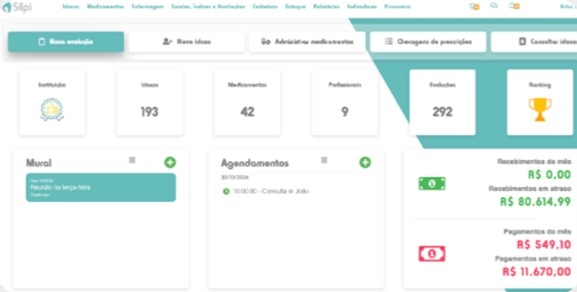
\includegraphics[width=0.85\textwidth]{figs/silpi.jpg}
	\label{fig:silpi}
	\fonte{Adaptado de SILPI (2025).}
\end{figure}

O sistema \textbf{Gestão 360 Social} \parencite{gestao360}, desenvolvido pela empresa SETA Sistemas, constitui uma plataforma voltada a instituições de assistência social, com foco na gestão integrada de acolhidos, voluntários, projetos e recursos financeiros. O sistema possibilita o cadastro detalhado de beneficiários, o controle de atendimentos, o acompanhamento da evolução dos acolhidos e a emissão de relatórios técnicos. Além disso, oferece integração com o CadÚnico e disponibiliza ferramentas para a prestação de contas, o planejamento de programas sociais e a conciliação bancária. Trata-se de uma solução escalável, capaz de ser adaptada a diferentes portes institucionais, promovendo maior transparência, eficiência e confiabilidade na gestão dos serviços oferecidos.

O sistema \textbf{ONG Fácil} \parencite{ongfacil2025} é uma plataforma on-line voltada à gestão de organizações não governamentais e instituições filantrópicas. A ferramenta oferece funcionalidades como controle de doações financeiras e materiais, cadastro de doadores, emissão de recibos, gestão de contas a pagar e a receber, e geração de relatórios financeiros. O sistema também dispõe de módulos para comunicação com doadores, campanhas de arrecadação e prestação de contas. Sua operação é integralmente baseada em nuvem, permitindo acesso remoto e seguro às informações. A interface apresenta estrutura simples e intuitiva, o que facilita o uso por equipes administrativas com diferentes níveis de familiaridade tecnológica.

Embora os sistemas analisados — \textit{Gestão 360 Social}, \textit{ONG Fácil} e \textit{SILPI – Sistemas Humanizados} — apresentem funcionalidades relevantes para a administração e o apoio assistencial em instituições sociais e filantrópicas, verificou-se que nenhum deles contempla integralmente as necessidades operacionais do Lar São Vicente de Paulo. As soluções existentes priorizam, em maior ou menor grau, aspectos relacionados à gestão administrativa, como controle financeiro, gerenciamento de doações e emissão de relatórios institucionais.  

No caso do \textit{SILPI}, embora se destaque por ser uma plataforma voltada especificamente à gestão de Instituições de Longa Permanência para Idosos (ILPIs), oferecendo recursos assistenciais como prontuário eletrônico, controle de medicamentos e registro da evolução clínica, ainda assim não atende plenamente às demandas particulares do Lar São Vicente de Paulo. Entre as lacunas observadas, ressaltam-se a ausência de funcionalidades voltadas à personalização do acompanhamento dos residentes, à integração com processos internos da instituição e à adaptação a fluxos de trabalho locais.  

Dessa forma, evidencia-se a necessidade de desenvolver um sistema que una a eficiência administrativa à gestão humanizada e individualizada dos residentes, atendendo de forma abrangente às especificidades funcionais e assistenciais de uma ILPI.

\section{Descrição dos Principais Problemas}

A ausência de um sistema informatizado específico para o gerenciamento das atividades do Lar São Vicente de Paulo tem ocasionado diversas dificuldades operacionais e administrativas, comprometendo a eficiência dos serviços prestados e a qualidade do atendimento aos idosos acolhidos. Durante o levantamento de requisitos e as visitas técnicas à instituição, observou-se que a gestão das informações é predominantemente manual, sendo realizada por meio de planilhas eletrônicas e registros físicos. Esse modelo de controle favorece a ocorrência de falhas, como a perda de dados, a duplicidade de registros e o preenchimento incorreto de informações essenciais.

Outro problema identificado refere-se à falta de integração entre os diferentes setores da instituição, como saúde, administração, assistência social e almoxarifado. A atuação isolada desses departamentos dificulta a comunicação interna, retarda a execução de processos e inviabiliza a tomada de decisões baseadas em dados consolidados. Além disso, a gestão de medicamentos, prescrições e prontuários clínicos é realizada de forma fragmentada, sem o suporte de um sistema que permita o acompanhamento histórico e a rastreabilidade das informações relacionadas aos residentes.

No campo financeiro, a administração de receitas, despesas, doações e prestações de contas ocorre sem o auxílio de ferramentas automatizadas, o que dificulta a transparência, o controle contábil e a elaboração de relatórios gerenciais. Essa limitação reflete também na impossibilidade de gerar indicadores de desempenho, relatórios de ocupação e análises sobre o consumo de recursos, restringindo o planejamento estratégico e a otimização dos processos internos. Soma-se a isso a baixa eficiência na captação e fidelização de doadores, já que o registro e o acompanhamento das doações são pouco estruturados, comprometendo a comunicação com apoiadores e a execução de campanhas de arrecadação eficazes.

Outro aspecto relevante diz respeito às restrições financeiras enfrentadas pela instituição, que inviabilizam a adoção de soluções comerciais disponíveis no mercado. Os sistemas existentes, embora ofereçam funcionalidades avançadas, possuem custos de licenciamento, manutenção e suporte técnico incompatíveis com a realidade orçamentária de uma entidade filantrópica. Assim, torna-se inviável a contratação ou personalização de softwares pagos, o que reforça a necessidade do desenvolvimento de uma solução própria, gratuita e sob medida para o contexto institucional.

Além disso, constatou-se que a comunicação interna entre os colaboradores ainda depende de meios informais, como bilhetes, telefonemas ou reuniões presenciais. Essa prática pode gerar atrasos, ruídos de comunicação e retrabalho, especialmente em situações que exigem respostas imediatas. Diante desse conjunto de fragilidades, evidencia-se a necessidade de desenvolver um sistema informatizado integrado e personalizado, capaz de atender às demandas específicas do Lar São Vicente de Paulo, assegurando maior eficiência administrativa, segurança da informação e continuidade da assistência humanizada aos idosos acolhidos.

\subsection{Descrição dos Requisitos Não Funcionais}

Os requisitos não funcionais abrangem os atributos de qualidade e desempenho do sistema, sendo responsáveis por assegurar que o software opere de forma eficiente, segura e estável. Segundo \textcite{PaulaFilho2015ES}, esses requisitos devem ser expressos de maneira precisa e, sempre que possível, quantitativa, uma vez que sua mensuração contribui para o controle da qualidade do produto final.

\begin{citacao}
	Os requisitos não funcionais surgem das necessidades dos usuários, que se devem a restrições orçamentárias, políticas organizacionais, necessidade de interoperabilidade com outros sistemas de software ou hardware, ou fatores externos, como normas de segurança (\textit{safety}) ou legislação relativa à privacidade. 
	\textcite[p.~91]{Sommerville2018ES10} 
\end{citacao}

O \textit{SeniorCareManager} foi desenvolvido em linguagem \textit{C\#} com arquitetura orientada a serviços, garantindo robustez e escalabilidade. O sistema utiliza um banco de dados relacional gratuito, adequado à realidade financeira das instituições filantrópicas, assegurando o armazenamento eficiente de informações sem comprometer a performance.  

Em relação ao desempenho, o sistema foi projetado para apresentar tempo de resposta inferior a três segundos para as principais operações e disponibilidade mínima de 99,8\%, assegurando acesso contínuo às informações. Em casos de falhas, o tempo máximo para correção ou atualização é de sete dias úteis, o que garante a manutenção da estabilidade e a confiança dos usuários.

A segurança das informações constitui um dos pilares do projeto. O controle de acesso é realizado por meio de autenticação baseada em tokens JWT (JSON Web Token), assegurando a integridade das sessões e a proteção contra acessos indevidos. Todas as transações são registradas em logs de auditoria, possibilitando o rastreamento de eventos, modificações e acessos ao sistema.  

A privacidade dos dados dos residentes é preservada em conformidade com a Lei nº 13.709/2018 — Lei Geral de Proteção de Dados Pessoais (LGPD) \textcite{brasil2018lgpd}, sendo vedado o compartilhamento de informações sensíveis sem autorização expressa.  

O sistema é compatível com diferentes navegadores e dispositivos, permitindo seu uso em computadores, tablets e smartphones. Além disso, a interface foi desenvolvida segundo princípios de usabilidade e design responsivo, favorecendo a experiência do usuário e a inclusão digital de profissionais de diferentes níveis de familiaridade tecnológica.  

A supervisão e validação de dados são realizadas por administradores autorizados, garantindo a qualidade das informações inseridas. Assim, o \textit{SeniorCareManager} alia desempenho, segurança e acessibilidade, constituindo uma solução tecnológica estável, ética e socialmente responsável.

A fim de assegurar a qualidade, robustez e confiabilidade do sistema proposto, torna-se imprescindível a definição clara dos requisitos não funcionais. Esses requisitos estabelecem parâmetros essenciais relacionados ao desempenho, segurança, disponibilidade e integridade das informações, servindo como base para orientar decisões arquiteturais e garantir que o sistema atenda às expectativas de uso em ambientes reais. O Quadro~\ref{quad:requisitos_nao_funcionais} apresenta a consolidação dos principais requisitos não funcionais identificados ao longo do processo de análise, ressaltando aspectos fundamentais para o funcionamento adequado e sustentável da solução.


\begin{quadro}[H]
	\centering
	\caption{Requisitos Não Funcionais}
	\label{quad:requisitos_nao_funcionais}
	\begin{tabularx}{\textwidth}{|l|X|}
		\hline
		\textbf{Requisitos Não Funcionais} & \textbf{Descrição} \\ \hline
		
		Desempenho & Garantir tempos de resposta rápidos para consultas e transações, mantendo alta eficiência. \\ \hline
		
		Segurança & Implementar medidas robustas, como controle de acesso e criptografia, para proteger dados sensíveis. \\ \hline
		
		Escalabilidade & Capacidade de lidar com um aumento substancial no volume de dados e transações. \\ \hline
		
		Disponibilidade & Assegurar que o banco de dados esteja acessível a maior parte do tempo, minimizando períodos de inatividade. \\ \hline
		
		Consistência & Manter a integridade e a consistência dos dados, garantindo precisão e atualização constante. \\ \hline
		
		Backup e Restauração & Estabelecer procedimentos eficientes para backup regular e recuperação rápida em caso de falhas. \\ \hline
	\end{tabularx}
	
	\fonte{Elaborado pelos autores.}
\end{quadro}


\subsection{Descrição dos Requisitos Funcionais}

Os requisitos funcionais representam uma das etapas mais importantes no processo de desenvolvimento de sistemas, uma vez que permitem identificar as necessidades dos usuários e definir as funcionalidades específicas que o software deverá executar. De acordo com \textcite{Sommerville2018ES10}, tais requisitos estabelecem uma base sólida para o planejamento, a implementação e os testes, garantindo que o produto final esteja alinhado às expectativas e aos objetivos do projeto.

O sistema \textit{SeniorCareManager} foi projetado para otimizar o gerenciamento das atividades do Lar dos Velhinhos São Vicente de Paulo e da APAE de Jales, integrando processos administrativos e assistenciais em uma única plataforma. Dessa forma, seus requisitos funcionais delineiam os serviços e operações essenciais que devem ser disponibilizados aos usuários, assegurando eficiência, rastreabilidade e segurança das informações.

Entre as funcionalidades principais, destacam-se os módulos de cadastro e manutenção de dados, que permitem incluir, editar e excluir registros de residentes, colaboradores, familiares, fornecedores e doações. Essas operações são realizadas por meio de botões de ação intuitivos, que facilitam o uso por diferentes perfis de profissionais da instituição.  

O sistema também dispõe de um módulo de prontuário eletrônico, no qual enfermeiros e cuidadores podem registrar e consultar informações clínicas, evoluções, prescrições, planos de cuidado e histórico vacinal. Essa estrutura segue a lógica dos modelos do \textit{e-SUS Atenção Primária} \textcite{ministeriosaude2023esus}, adaptada às particularidades da assistência em Instituições de Longa Permanência para Idosos (ILPIs).

Outros recursos incluem o módulo de estoque, destinado ao controle de insumos, medicamentos e materiais de uso contínuo; o módulo de compras e doações, que organiza o recebimento, a distribuição e a prestação de contas dos recursos; e o módulo de vacinas, que gerencia as campanhas de imunização, alertas de vencimento e registros de aplicação.  

O sistema incorpora ainda mecanismos de pesquisa e filtragem de informações, com campos dinâmicos e categorização por grupos e subgrupos, permitindo consultas rápidas e precisas. A acessibilidade também é um aspecto prioritário, assegurando que o \textit{SeniorCareManager} possa ser utilizado por diferentes perfis de usuários, incluindo profissionais com limitações visuais ou motoras.  

Por fim, o sistema mantém integração com serviços externos, como geolocalização para registro de visitas domiciliares e notificações automáticas via e-mail, ampliando a conectividade e a eficiência das rotinas institucionais.


\chapter{Visão de Caso de Uso - UML}

O entendimento profundo de um sistema é crucial para o sucesso de qualquer projeto de desenvolvimento de software. Nesse contexto, a Linguagem de Modelagem Unificada (UML) configura-se como uma ferramenta essencial para representar visualmente a estrutura e as interações entre os componentes de um sistema. Conforme afirmam \textcite{Guedes2018}, a UML possibilita a modelagem clara e estruturada de artefatos de software, contribuindo para o entendimento e a comunicação entre os envolvidos no projeto. De forma complementar, \textcite{Miro2024} destaca que “desenvolvedores criam diagramas UML para entender projetos, arquitetura de código e propostas de implementação de sistemas de software complexos.”

A análise apresentada a seguir dedica-se à exploração dos principais diagramas da UML aplicados no desenvolvimento do sistema. Esses diagramas desempenham um papel fundamental na compreensão da estrutura e na narrativa do processo de desenvolvimento, oferecendo uma visão aprofundada de sua arquitetura. Ao examinar cada diagrama, busca-se desvendar não apenas a organização técnica, mas também a lógica e a dinâmica subjacentes ao desenvolvimento, proporcionando uma base sólida para a compreensão abrangente do projeto.

\section{Diagrama de Classes}

O diagrama de classes é fundamental na UML, sendo essencial para a criação dos demais diagramas do conjunto. Seu principal enfoque está em permitir a visualização das classes que comporão o sistema, juntamente com seus respectivos atributos e métodos, além de demonstrar como essas classes se relacionam, complementam e transmitem informações entre si.

\begin{citacao}
	Seu principal enfoque está em permitir a visualização das classes que comporão o sistema com seus respectivos atributos e métodos, bem como em demonstrar como as classes do diagrama se relacionam, complementam e transmitem informações entre si. Esse diagrama apresenta uma visão estática de como as classes estão organizadas, preocupando-se em como definir a estrutura lógica delas. (\textcite[p.~133]{Guedes2018})
\end{citacao}

De acordo com \textcite{Sommerville2018ES10}, os diagramas de classes são estruturados em torno de um retângulo simples que representa uma classe. No interior desse retângulo, o nome da classe é apresentado na parte superior, seguido pelos atributos e seus tipos na área intermediária. As relações entre as classes são representadas por linhas conectando os retângulos, indicando as associações entre elas e demonstrando como os elementos se interligam no modelo estático.

O diagrama de classes apresentado descreve uma arquitetura robusta e modular que integra informações administrativas, assistenciais, clínicas e operacionais do sistema. No núcleo do modelo destaca-se a classe \texttt{Resident}, responsável por concentrar os dados pessoais, sociais e de saúde dos residentes. Essa classe se relaciona diretamente com entidades auxiliares, como \texttt{Religion}, \texttt{Sex}, \texttt{Ethnicity}, \texttt{HealthInsurancePlan} e \texttt{NursingCarePlan}, permitindo representar características individuais, plano de saúde, cuidados prescritos e dimensões culturais. A estrutura do residente também é estendida por classes especializadas, como \texttt{ResidentRelative}, que registra contatos familiares e vínculos de parentesco, \texttt{ResidentAllergy}, que mapeia alergias vinculadas à classe \texttt{Allergy}, e \texttt{CID10}, utilizada para classificação padronizada de diagnósticos médicos.

A dimensão assistencial do modelo é reforçada pelas classes \texttt{Employee}, \texttt{Position}, \texttt{User} e \texttt{TechnicalResponsibility}, que compõem o conjunto de profissionais do sistema. Essas classes representam funções institucionais, níveis de acesso, responsabilidades técnicas e informações de cadastro, evidenciando como os colaboradores interagem com o sistema e executam ações clínicas e administrativas. Elementos como \texttt{Prescription} e \texttt{NursingService} reforçam o subsistema de cuidado, permitindo o registro estruturado de intervenções, serviços e condutas.

A segunda grande área modelada refere-se ao \textit{módulo de estoque e suprimentos}. Nessa seção do diagrama, encontram-se classes como \texttt{Product}, \texttt{ProductGroup}, \texttt{ProductType}, \texttt{ProductBatch}, \texttt{Supplier}, \texttt{Invoice}, \texttt{Carrier} e \texttt{UnitOfMeasure}, que juntas garantem o registro completo de produtos, fornecedores, unidades de medida, lotes e movimentações fiscais. O ciclo de solicitação e movimentação de materiais é detalhado por classes como \texttt{PurchaseRequest}, \texttt{PurchaseRequestItem}, \texttt{StockRequest}, \texttt{StockRequestItem}, \texttt{StockMovement} e \texttt{StockDocument}. Os enumeradores associados descrevem estados dos processos, tipos de movimentação e etapas de aprovação, permitindo rastreabilidade precisa de entradas, saídas, ajustes e solicitações internas.

De maneira geral, o diagrama revela um sistema amplamente integrado, no qual módulos assistenciais, administrativos e logísticos se articulam de maneira coesa. As associações, multiplicidades e enumerações indicam regras de negócio específicas, vínculos hierárquicos, dependências obrigatórias e processos padronizados. Assim, o diagrama de classes fornece uma visão estática abrangente da estrutura do sistema, desempenhando papel fundamental na compreensão dos componentes que o compõem e nas inter-relações que sustentam seu funcionamento, conforme enfatizado por \textcite{Guedes2018} e \textcite{Sommerville2018ES10}.

\begin{figure}[H]
	%\centering
	\caption{Diagrama de Classe}
	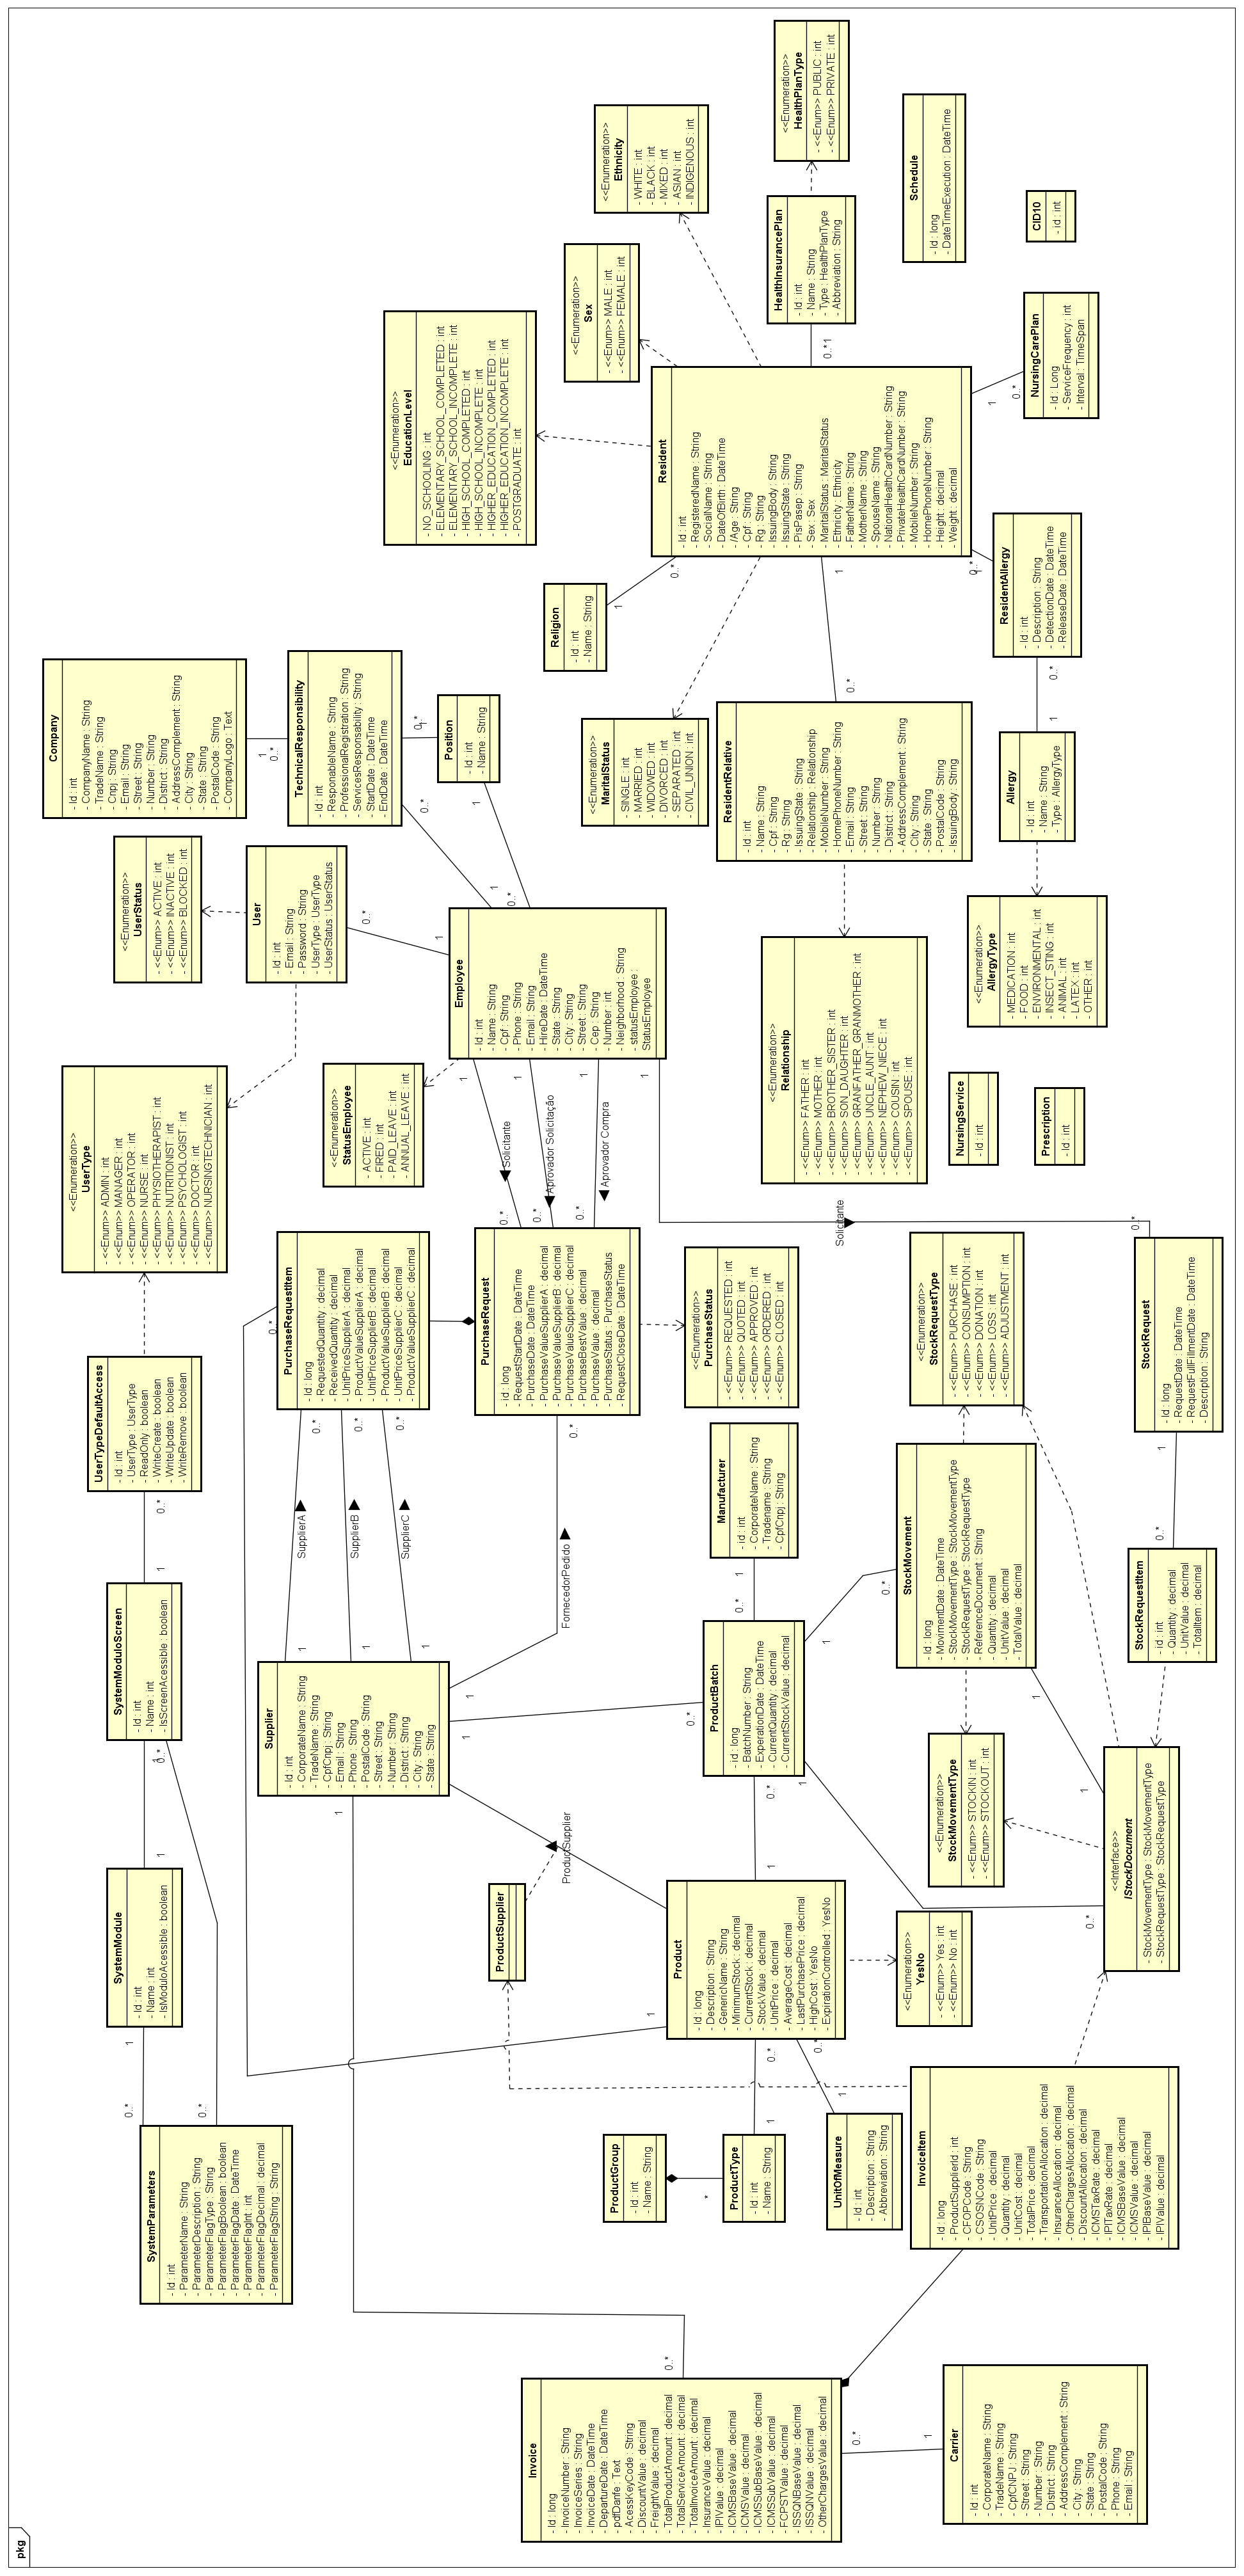
\includegraphics[width=0.7\textwidth]{figs/ClassDiagram.png}
	\label{fig:diagramaclasse}
	\fonte{Elaborado pelos autores (2025).}
\end{figure}

\section{Dicionário de Classes}

O \textit{Quadro}~\ref{quad:dicionario-de-dados-da-entidade-product} apresenta o dicionário de dados da entidade \textit{Product}, descrevendo seus atributos, respectivos tipos e funções no modelo de domínio do sistema. Esse mapeamento estrutural possibilita compreender como as informações sobre os produtos são armazenadas, organizadas e utilizadas pelas camadas de persistência e regras de negócio, garantindo padronização e consistência no desenvolvimento do software.

% Quadro 2
\begin{quadro}[H]
	\caption[Entidade Product]{Dicionário de dados da entidade Product}
	\label{quad:dicionario-de-dados-da-entidade-product}
	\begin{tabular}{|p{0.22\textwidth}|p{0.18\textwidth}|p{0.50\textwidth}|}
		\hline
		\textbf{Atributo} & \textbf{Tipo} & \textbf{Descrição} \\ \hline
		
		Id & long & Código único que identifica um produto. \\ \hline
		
		Description & String & Nome comercial ou descrição principal do produto (ex.: “Dipirona 500mg Caixa com 20”). \\ \hline
		
		GenericName & String & Nome genérico ou princípio ativo do produto (ex.: “Dipirona Monoidratada”). \\ \hline
		
		MinimumStock & decimal & Quantidade mínima ideal que deve haver deste produto em estoque. \\ \hline
		
		CurrentStock & decimal & Quantidade total atual deste produto em estoque (soma de todos os lotes). \\ \hline
		
		StockValue & decimal & Valor monetário total do estoque atual para este produto. \\ \hline
		
		UnitPrice & decimal & Preço de venda unitário do produto. \\ \hline
		
		AverageCost & decimal & Custo médio de aquisição do produto, ponderado pelas compras. \\ \hline
		
		LastPurchasePrice & decimal & Preço unitário da última compra realizada para este produto. \\ \hline
		
		HighCost & YesNo & Enum (Sim/Não) que indica se o produto é classificado como de alto custo. \\ \hline
		
		ExpirationControlled & YesNo & Enum (Sim/Não) que indica se o produto requer controle de data de validade. \\ \hline
		
	\end{tabular}
	\fonte{Elaborado pelos autores.}
\end{quadro}

O \textit{Quadro}~\ref{quad:dicionario-de-dados-da-entidade-productbatch} apresenta o dicionário de dados da entidade \textit{ProductBatch}, responsável por representar os lotes associados a cada produto. Seus atributos permitem o controle detalhado de identificação, validade, quantidade e valor em estoque, assegurando rastreabilidade e precisão nos processos de gestão de materiais.

\begin{quadro}[H]
	\caption[Entidade ProductBatch]{Dicionário de dados da entidade ProductBatch}
	\label{quad:dicionario-de-dados-da-entidade-productbatch}
	\begin{tabular}{|p{0.22\textwidth}|p{0.18\textwidth}|p{0.50\textwidth}|}
		\hline
		\textbf{Atributo} & \textbf{Tipo} & \textbf{Descrição} \\ \hline
		
		Id & long & Código único que identifica um lote de produto. \\ \hline
		BatchNumber & String & Código ou número que identifica o lote específico do fabricante. \\ \hline
		ExpirationDate & DateTime & Data de validade do lote. \\ \hline
		CurrentQuantity & decimal & Quantidade atual de itens restantes neste lote específico. \\ \hline
		CurrentStockValue & decimal & Valor monetário total do estoque restante neste lote. \\ \hline
		
	\end{tabular}
	\fonte{Elaborado pelos autores.}
\end{quadro}


O \textit{Quadro}~\ref{quad:dicionario-de-dados-da-entidade-producttype} descreve a entidade \textit{ProductType}, utilizada para classificar os produtos conforme sua natureza ou finalidade. Essa categorização é fundamental para organizar o catálogo do sistema, apoiar regras de negócio específicas e facilitar o gerenciamento de diferentes grupos de itens.

\begin{quadro}[H]
	\caption[Entidade ProductType]{Dicionário de dados da entidade ProductType}
	\label{quad:dicionario-de-dados-da-entidade-producttype}
	\begin{tabular}{|p{0.22\textwidth}|p{0.18\textwidth}|p{0.50\textwidth}|}
		\hline
		\textbf{Atributo} & \textbf{Tipo} & \textbf{Descrição} \\ \hline
		
		Id & int & Código único que identifica o tipo de produto. \\ \hline
		Name & String & Nome que descreve o tipo do produto (ex.: “Medicamento”, “Material de Higiene”). \\ \hline
		
	\end{tabular}
	\fonte{Elaborado pelos autores.}
\end{quadro}


O \textit{Quadro}~\ref{quad:dicionario-de-dados-da-entidade-unitofmeasure} apresenta o dicionário de dados da entidade \textit{UnitOfMeasure}, que define as unidades de medida utilizadas pelo sistema. A padronização dessas unidades garante consistência na movimentação de estoque, nos cálculos de valor e na integração entre diferentes módulos do software.

\begin{quadro}[H]
	\caption[Entidade UnitOfMeasure]{Dicionário de dados da entidade UnitOfMeasure}
	\label{quad:dicionario-de-dados-da-entidade-unitofmeasure}
	\begin{tabular}{|p{0.22\textwidth}|p{0.18\textwidth}|p{0.50\textwidth}|}
		\hline
		\textbf{Atributo} & \textbf{Tipo} & \textbf{Descrição} \\ \hline
		
		Id & int & Código único que identifica a unidade de medida. \\ \hline
		Description & String & Descrição por extenso da unidade de medida (ex.: “Quilograma”, “Unidade”). \\ \hline
		Abbreviation & String & Abreviatura da unidade de medida (ex.: “Kg”, “Un”). \\ \hline
		
	\end{tabular}
	\fonte{Elaborado pelos autores.}
\end{quadro}


O \textit{Quadro}~\ref{quad:dicionario-de-dados-da-entidade-manufacturer} mostra o dicionário de dados da entidade \textit{Manufacturer}, responsável por registrar as informações cadastrais de fabricantes e laboratórios. A correta identificação desses fornecedores é essencial para a rastreabilidade dos produtos e para assegurar conformidade documental e regulatória.

\begin{quadro}[H]
	\caption[Entidade Manufacturer]{Dicionário de dados da entidade Manufacturer}
	\label{quad:dicionario-de-dados-da-entidade-manufacturer}
	\begin{tabular}{|p{0.22\textwidth}|p{0.18\textwidth}|p{0.50\textwidth}|}
		\hline
		\textbf{Atributo} & \textbf{Tipo} & \textbf{Descrição} \\ \hline
		
		Id & int & Código único que identifica um fabricante ou laboratório. \\ \hline
		CorporateName & String & Nome legal e formal do fabricante (Razão Social). \\ \hline
		Tradename & String & Nome de marca ou comercial do fabricante (Nome Fantasia). \\ \hline
		CpfCnpj & String & Número do CPF ou CNPJ do fabricante. \\ \hline
		
	\end{tabular}
	\fonte{Elaborado pelos autores.}
\end{quadro}

O \textit{Quadro}~\ref{quad:dicionario-de-dados-da-entidade-stockmovement} apresenta o dicionário de dados da entidade \textit{StockMovement}, que registra todas as movimentações realizadas no estoque. Seus atributos permitem identificar o tipo de movimentação, sua origem, os valores envolvidos e o documento que deu causa à operação, fornecendo suporte essencial para auditoria, rastreabilidade e controle financeiro.


\begin{quadro}[H]
	\caption[Entidade StockMovement]{Dicionário de dados da entidade StockMovement}
	\label{quad:dicionario-de-dados-da-entidade-stockmovement}
	\begin{tabular}{|p{0.22\textwidth}|p{0.18\textwidth}|p{0.50\textwidth}|}
		\hline
		\textbf{Atributo} & \textbf{Tipo} & \textbf{Descrição} \\ \hline
		
		Id & long & Código único que identifica uma movimentação de estoque. \\ \hline
		MovimentDate & DateTime & Data e hora em que a movimentação de estoque ocorreu. \\ \hline
		StockMovementType & StockMovementType & Enum que define o tipo de movimentação (Entrada ou Saída). \\ \hline
		StockRequestType & StockRequestType & Enum que define a origem ou motivo da movimentação (Compra, Consumo, Perda, etc.). \\ \hline
		ReferenceDocument & String & Número do documento de referência que gerou a movimentação (ex.: Nota Fiscal). \\ \hline
		Quantity & decimal & Quantidade de produto que foi movimentada. \\ \hline
		UnitValue & decimal & Valor unitário do produto na movimentação. \\ \hline
		TotalValue & decimal & Valor total da movimentação (Quantidade × Valor Unitário). \\ \hline
		
	\end{tabular}
	\fonte{Elaborado pelos autores.}
\end{quadro}

O \textit{Quadro}~\ref{quad:dicionario-de-dados-da-entidade-supplier} apresenta o dicionário de dados da entidade \textit{Supplier}, que armazena as informações cadastrais de fornecedores. Esses dados incluem identificação jurídica, contatos e endereço completo, permitindo ao sistema manter registros confiáveis e essenciais para processos de compras, auditorias e conformidade regulatória.

\begin{quadro}[H]
	\caption[Entidade Supplier]{Dicionário de dados da entidade Supplier}
	\label{quad:dicionario-de-dados-da-entidade-supplier}
	\begin{tabular}{|p{0.22\textwidth}|p{0.18\textwidth}|p{0.50\textwidth}|}
		\hline
		\textbf{Atributo} & \textbf{Tipo} & \textbf{Descrição} \\ \hline
		
		Id & int & Código único que identifica um fornecedor. \\ \hline
		CorporateName & String & Nome legal e formal do fornecedor (Razão Social). \\ \hline
		TradeName & String & Nome de marca pelo qual o fornecedor é conhecido (Nome Fantasia). \\ \hline
		CpfCnpj & String & Número de CPF ou CNPJ do fornecedor. \\ \hline
		Email & String & Endereço de e-mail principal de contato. \\ \hline
		Phone & String & Número de telefone principal de contato. \\ \hline
		PostalCode & String & Código de Endereçamento Postal (CEP). \\ \hline
		Street & String & Rua ou logradouro do endereço do fornecedor. \\ \hline
		Number & String & Número do endereço do fornecedor. \\ \hline
		District & String & Bairro do endereço do fornecedor. \\ \hline
		City & String & Cidade do endereço do fornecedor. \\ \hline
		State & String & Sigla do estado (UF) do endereço do fornecedor. \\ \hline
		
	\end{tabular}
	\fonte{Elaborado pelos autores.}
\end{quadro}

O \textit{Quadro}~\ref{quad:dicionario-de-dados-da-entidade-stockmovementtype} apresenta o enum \textit{StockMovementType}, utilizado para classificar as movimentações de estoque como entrada ou saída. Essa distinção é fundamental para o correto funcionamento das rotinas de controle de estoque, garantindo consistência nas operações e nos registros históricos.

\begin{quadro}[H]
	\caption[Enum StockMovementType]{Dicionário de dados do enum StockMovementType}
	\label{quad:dicionario-de-dados-da-entidade-stockmovementtype}
	\begin{tabular}{|p{0.28\textwidth}|p{0.12\textwidth}|p{0.48\textwidth}|}
		\hline
		\textbf{Valor} & \textbf{Tipo} & \textbf{Descrição} \\ \hline
		
		\texttt{STOCKIN} & int & Valor do enum que representa uma entrada de estoque. \\ \hline
		\texttt{STOCKOUT} & int & Valor do enum que representa uma saída de estoque. \\ \hline
		
	\end{tabular}
	\fonte{Elaborado pelos autores.}
\end{quadro}

O \textit{Quadro}~\ref{quad:dicionario-de-dados-da-entidade-stockrequesttype} descreve o enum \textit{StockRequestType}, que identifica a origem da movimentação de estoque. Essa categorização é essencial para diferenciar compras, consumos, doações, perdas e ajustes, permitindo análises e controles precisos sobre o comportamento do estoque.


\begin{quadro}[H]
	\caption[Enum StockRequestType]{Dicionário de dados do enum StockRequestType}
	\label{quad:dicionario-de-dados-da-entidade-stockrequesttype}
	\begin{tabular}{|p{0.28\textwidth}|p{0.12\textwidth}|p{0.48\textwidth}|}
		\hline
		\textbf{Valor} & \textbf{Tipo} & \textbf{Descrição} \\ \hline
		
		\texttt{PURCHASE} & int & Representa uma movimentação originada de compra. \\ \hline
		\texttt{CONSUMPTION} & int & Representa uma movimentação originada do consumo interno. \\ \hline
		\texttt{DONATION} & int & Representa uma movimentação originada de doação. \\ \hline
		\texttt{LOSS} & int & Representa uma baixa no estoque por perda ou avaria. \\ \hline
		\texttt{ADJUSTMENT} & int & Representa uma movimentação por ajuste de inventário. \\ \hline
		
	\end{tabular}
	\fonte{Elaborado pelos autores.}
\end{quadro}

O \textit{Quadro}~\ref{quad:dicionario-de-dados-da-entidade-purchaserequest} apresenta o dicionário de dados da entidade \textit{PurchaseRequest}, responsável por registrar o processo de requisição e fechamento de compras. Seus atributos contemplam as datas de abertura e conclusão, os valores obtidos nas cotações com diferentes fornecedores, o valor final contratado e o status da compra, oferecendo uma visão estruturada de todo o ciclo de aquisição.

\begin{quadro}[H]
	\caption[Entidade PurchaseRequest]{Dicionário de dados da entidade PurchaseRequest}
	\label{quad:dicionario-de-dados-da-entidade-purchaserequest}
	\begin{tabular}{|p{0.24\textwidth}|p{0.16\textwidth}|p{0.50\textwidth}|}
		\hline
		\textbf{Atributo} & \textbf{Tipo} & \textbf{Descrição} \\ \hline
		
		Id & long & Código único que identifica uma requisição de compra. \\ \hline
		RequestStartDate & DateTime & Data em que a requisição de compra foi iniciada. \\ \hline
		PurchaseDate & DateTime & Data em que a compra foi efetivamente realizada. \\ \hline
		PurchaseValueSupplierA & decimal & Valor total da cotação com o Fornecedor A. \\ \hline
		PurchaseValueSupplierB & decimal & Valor total da cotação com o Fornecedor B. \\ \hline
		PurchaseValueSupplierC & decimal & Valor total da cotação com o Fornecedor C. \\ \hline
		PurchaseBestValue & decimal & Melhor valor (menor) entre as cotações realizadas. \\ \hline
		PurchaseValue & decimal & Valor final pelo qual a compra foi fechada. \\ \hline
		PurchaseStatus & PurchaseStatus & Enum que indica o status atual do processo de compra. \\ \hline
		RequestCloseDate & DateTime & Data em que a requisição de compra foi concluída ou cancelada. \\ \hline
		
	\end{tabular}
	\fonte{Elaborado pelos autores.}
\end{quadro}

O \textit{Quadro}~\ref{quad:dicionario-de-dados-da-entidade-purchaserequestitem} apresenta o dicionário de dados da entidade \textit{PurchaseRequestItem}, que detalha os itens vinculados a uma requisição de compra. Nessa estrutura são descritas as quantidades solicitadas e recebidas, bem como os preços unitários e valores totais obtidos nas cotações com diferentes fornecedores, permitindo análise comparativa e transparência no processo de aquisição.

\begin{quadro}[H]
	\caption[Entidade PurchaseRequestItem]{Dicionário de dados da entidade PurchaseRequestItem}
	\label{quad:dicionario-de-dados-da-entidade-purchaserequestitem}
	\begin{tabular}{|p{0.24\textwidth}|p{0.16\textwidth}|p{0.50\textwidth}|}
		\hline
		\textbf{Atributo} & \textbf{Tipo} & \textbf{Descrição} \\ \hline
		
		Id & long & Código único que identifica um item dentro de uma requisição de compra. \\ \hline
		RequestedQuantity & decimal & Quantidade do produto que foi solicitada. \\ \hline
		ReceivedQuantity & decimal & Quantidade do produto que foi efetivamente recebida. \\ \hline
		UnitPriceSupplierA & decimal & Preço unitário do produto na cotação com o Fornecedor A. \\ \hline
		ProductValueSupplierA & decimal & Valor total do produto na cotação com o Fornecedor A. \\ \hline
		UnitPriceSupplierB & decimal & Preço unitário do produto na cotação com o Fornecedor B. \\ \hline
		ProductValueSupplierB & decimal & Valor total do produto na cotação com o Fornecedor B. \\ \hline
		UnitPriceSupplierC & decimal & Preço unitário do produto na cotação com o Fornecedor C. \\ \hline
		ProductValueSupplierC & decimal & Valor total do produto na cotação com o Fornecedor C. \\ \hline
		
	\end{tabular}
	\fonte{Elaborado pelos autores.}
\end{quadro}

O \textit{Quadro}~\ref{quad:dicionario-de-dados-da-entidade-employee} apresenta o dicionário de dados da entidade \textit{Employee}, responsável por armazenar as informações cadastrais dos colaboradores da instituição. Os atributos contemplam dados pessoais, de contato, endereço e situação funcional, servindo de base para os módulos de gestão de recursos humanos e controle de acesso ao sistema.

\begin{quadro}[H]
	\caption[Entidade Employee]{Dicionário de dados da entidade Employee}
	\label{quad:dicionario-de-dados-da-entidade-employee}
	\begin{tabular}{|p{0.24\textwidth}|p{0.16\textwidth}|p{0.50\textwidth}|}
		\hline
		\textbf{Atributo} & \textbf{Tipo} & \textbf{Descrição} \\ \hline
		
		Id & int & Código único que identifica um funcionário. \\ \hline
		Name & String & Nome completo do funcionário. \\ \hline
		Cpf & String & Número do CPF do funcionário. \\ \hline
		Phone & String & Telefone de contato do funcionário. \\ \hline
		Email & String & Endereço de e-mail do funcionário. \\ \hline
		HireDate & DateTime & Data em que o funcionário foi contratado. \\ \hline
		State & String & Estado (UF) do endereço do empregado. \\ \hline
		City & String & Cidade do endereço do empregado. \\ \hline
		Street & String & Rua do endereço do empregado. \\ \hline
		Cep & String & Código de Endereçamento Postal (CEP) do endereço do empregado. \\ \hline
		Number & int & Número do endereço do empregado. \\ \hline
		Neighborhood & String & Bairro ou vizinhança do endereço do empregado. \\ \hline
		statusEmployee & StatusEmployee & Enum que indica a situação atual do funcionário (Ativo, Demitido, etc.). \\ \hline
		
	\end{tabular}
	\fonte{Elaborado pelos autores.}
\end{quadro}

O \textit{Quadro}~\ref{quad:dicionario-de-dados-da-entidade-position} apresenta o dicionário de dados da entidade \textit{Position}, utilizada para representar os cargos existentes na instituição. Essa estrutura permite padronizar a nomenclatura de funções e apoiar rotinas de alocação de pessoal, hierarquia organizacional e controle de permissões no sistema.

\begin{quadro}[H]
	\caption[Entidade Position]{Dicionário de dados da entidade Position}
	\label{quad:dicionario-de-dados-da-entidade-position}
	\begin{tabular}{|p{0.24\textwidth}|p{0.16\textwidth}|p{0.50\textwidth}|}
		\hline
		\textbf{Atributo} & \textbf{Tipo} & \textbf{Descrição} \\ \hline
		
		Id & int & Código único que identifica um cargo na instituição. \\ \hline
		Name & String & Nome do cargo (ex.: ``Enfermeiro Chefe'', ``Fisioterapeuta''). \\ \hline
		
	\end{tabular}
	\fonte{Elaborado pelos autores.}
\end{quadro}

O \textit{Quadro}~\ref{quad:dicionario-de-dados-da-entidade-purchasestatus} apresenta o enum \textit{PurchaseStatus}, utilizado para representar as etapas do processo de compra dentro do sistema. Esses estados permitem acompanhar a evolução da requisição, desde sua abertura até o encerramento, garantindo rastreabilidade e controle das movimentações de aquisição.

\begin{quadro}[H]
	\caption[Enum PurchaseStatus]{Dicionário de dados do enum PurchaseStatus}
	\label{quad:dicionario-de-dados-da-entidade-purchasestatus}
	\begin{tabular}{|p{0.30\textwidth}|p{0.10\textwidth}|p{0.48\textwidth}|}
		\hline
		\textbf{Valor} & \textbf{Tipo} & \textbf{Descrição} \\ \hline
		
		\texttt{REQUESTED} & int & Indica que a compra foi solicitada. \\ \hline
		\texttt{QUOTED} & int & Indica que a compra está na fase de cotação. \\ \hline
		\texttt{APPROVED} & int & Indica que a compra foi aprovada. \\ \hline
		\texttt{ORDERED} & int & Indica que o pedido de compra foi enviado ao fornecedor. \\ \hline
		\texttt{CLOSED} & int & Indica que o processo de compra foi finalizado. \\ \hline
		
	\end{tabular}
	\fonte{Elaborado pelos autores.}
\end{quadro}

O \textit{Quadro}~\ref{quad:dicionario-de-dados-da-entidade-yesno} descreve o enum \textit{YesNo}, utilizado para representar respostas booleanas em formato textual dentro do sistema. Essa estrutura padroniza o uso das opções “Sim” e “Não” em diversos módulos e funcionalidades.

\begin{quadro}[H]
	\caption[Enum YesNo]{Dicionário de dados do enum YesNo}
	\label{quad:dicionario-de-dados-da-entidade-yesno}
	\begin{tabular}{|p{0.30\textwidth}|p{0.10\textwidth}|p{0.48\textwidth}|}
		\hline
		\textbf{Valor} & \textbf{Tipo} & \textbf{Descrição} \\ \hline
		
		\texttt{Yes} & int & Representa a resposta “Sim”. \\ \hline
		\texttt{No} & int & Representa a resposta “Não”. \\ \hline
		
	\end{tabular}
	\fonte{Elaborado pelos autores.}
\end{quadro}

O \textit{Quadro}~\ref{quad:dicionario-de-dados-da-entidade-stockrequest} apresenta o dicionário de dados da entidade \textit{StockRequest}, que representa solicitações de saída de estoque. Seus atributos contemplam datas, descrição e informações essenciais para rastrear a operação e justificar a movimentação dos produtos.

\begin{quadro}[H]
	\caption[Entidade StockRequest]{Dicionário de dados da entidade StockRequest}
	\label{quad:dicionario-de-dados-da-entidade-stockrequest}
	\begin{tabular}{|p{0.24\textwidth}|p{0.16\textwidth}|p{0.50\textwidth}|}
		\hline
		\textbf{Atributo} & \textbf{Tipo} & \textbf{Descrição} \\ \hline
		
		Id & long & Código único que identifica uma requisição de estoque (saída). \\ \hline
		RequestDate & DateTime & Data em que a requisição foi feita. \\ \hline
		RequestFullFillmentDate & DateTime & Data em que a requisição foi atendida. \\ \hline
		Description & String & Descrição ou justificativa da requisição de estoque. \\ \hline
		
	\end{tabular}
	\fonte{Elaborado pelos autores.}
\end{quadro}

O \textit{Quadro}~\ref{quad:dicionario-de-dados-da-entidade-stockrequestitem} apresenta o dicionário de dados da entidade \textit{StockRequestItem}, que descreve os itens incluídos em uma requisição de estoque. Os atributos indicam quantidades e valores associados a cada produto solicitado.

\begin{quadro}[H]
	\caption[Entidade StockRequestItem]{Dicionário de dados da entidade StockRequestItem}
	\label{quad:dicionario-de-dados-da-entidade-stockrequestitem}
	\begin{tabular}{|p{0.24\textwidth}|p{0.16\textwidth}|p{0.50\textwidth}|}
		\hline
		\textbf{Atributo} & \textbf{Tipo} & \textbf{Descrição} \\ \hline
		
		Id & int & Código único que identifica um item da requisição. \\ \hline
		Quantity & decimal & Quantidade do produto solicitada. \\ \hline
		UnitValue & decimal & Valor unitário do produto no momento da requisição. \\ \hline
		TotalItem & decimal & Valor total do item (Quantidade × Valor Unitário). \\ \hline
		
	\end{tabular}
	\fonte{Elaborado pelos autores.}
\end{quadro}

O \textit{Quadro}~\ref{quad:dicionario-de-dados-da-entidade-invoice} apresenta o dicionário de dados da entidade \textit{Invoice}, que registra todas as informações referentes às notas fiscais. Seus atributos contemplam identificação, datas, impostos, valores de produtos e serviços, seguro, frete e demais encargos, permitindo controle detalhado das operações fiscais e contábeis.

\begin{quadro}[H]
	\caption[Entidade Invoice]{Dicionário de dados da entidade Invoice}
	\label{quad:dicionario-de-dados-da-entidade-invoice}
	\begin{tabular}{|p{0.23\textwidth}|p{0.15\textwidth}|p{0.52\textwidth}|}
		\hline
		\textbf{Atributo} & \textbf{Tipo} & \textbf{Descrição} \\ \hline
		
		Id & long & Código único que identifica uma nota fiscal. \\ \hline
		InvoiceNumber & String & Número da nota fiscal. \\ \hline
		InvoiceSeries & String & Série da nota fiscal. \\ \hline
		InvoiceDate & DateTime & Data de emissão da nota fiscal. \\ \hline
		DepartureDate & DateTime & Data de envio da mercadoria. \\ \hline
		pdfDanfe & Text & Conteúdo do PDF da DANFE. \\ \hline
		AcessKeyCode & String & Chave de acesso (44 dígitos). \\ \hline
		DiscountValue & decimal & Valor total do desconto. \\ \hline
		FreightValue & decimal & Valor total do frete. \\ \hline
		TotalProductAmount & decimal & Valor total dos produtos. \\ \hline
		TotalServiceAmount & decimal & Valor total dos serviços. \\ \hline
		TotalInvoiceAmount & decimal & Valor total da nota fiscal. \\ \hline
		InsuranceValue & decimal & Valor do seguro da carga. \\ \hline
		IPIValue & decimal & Valor total do IPI. \\ \hline
		ICMSBaseValue & decimal & Base de cálculo do ICMS. \\ \hline
		ICMSValue & decimal & Valor total do ICMS. \\ \hline
		ICMSSubBaseValue & decimal & Base de cálculo do ICMS-ST. \\ \hline
		ICMSSubValue & decimal & Valor do ICMS-ST. \\ \hline
		FCPSTValue & decimal & Valor do FCP-ST. \\ \hline
		ISSQNBaseValue & decimal & Base de cálculo do ISSQN. \\ \hline
		ISSQNValue & decimal & Valor total do ISSQN. \\ \hline
		OtherChargesValue & decimal & Outras despesas acessórias. \\ \hline
		
	\end{tabular}
	\fonte{Elaborado pelos autores.}
\end{quadro}

O \textit{Quadro}~\ref{quad:dicionario-de-dados-da-entidade-invoiceitem} apresenta o dicionário de dados da entidade \textit{InvoiceItem}, que descreve cada item pertencente a uma nota fiscal. São detalhados valores unitários, quantidades, impostos, rateios e demais elementos fiscais que compõem o cálculo do item.

\begin{quadro}[H]
	\caption[Entidade InvoiceItem]{Dicionário de dados da entidade InvoiceItem}
	\label{quad:dicionario-de-dados-da-entidade-invoiceitem}
	\begin{tabular}{|p{0.23\textwidth}|p{0.15\textwidth}|p{0.52\textwidth}|}
		\hline
		\textbf{Atributo} & \textbf{Tipo} & \textbf{Descrição} \\ \hline
		
		Id & long & Código único do item na nota fiscal. \\ \hline
		ProductSupplierId & int & ID do produto conforme cadastro do fornecedor. \\ \hline
		CFOPCode & String & Código Fiscal de Operações e Prestações. \\ \hline
		CSOSNCode & String & Código de Situação da Operação (Simples Nacional). \\ \hline
		UnitPrice & decimal & Preço unitário na nota fiscal. \\ \hline
		Quantity & decimal & Quantidade do produto na nota fiscal. \\ \hline
		UnitCost & decimal & Custo unitário considerando impostos e despesas. \\ \hline
		TotalPrice & decimal & Valor total do item. \\ \hline
		TransportationAllocation & decimal & Rateio do frete. \\ \hline
		InsuranceAllocation & decimal & Rateio do seguro. \\ \hline
		OtherChargesAllocation & decimal & Rateio de outras despesas. \\ \hline
		DiscountAllocation & decimal & Rateio do desconto. \\ \hline
		ICMSTaxRate & decimal & Alíquota do ICMS. \\ \hline
		IPITaxRate & decimal & Alíquota do IPI. \\ \hline
		ICMSBaseValue & decimal & Base de cálculo do ICMS. \\ \hline
		ICMSValue & decimal & Valor do ICMS. \\ \hline
		IPIBaseValue & decimal & Base de cálculo do IPI. \\ \hline
		IPIValue & decimal & Valor do IPI. \\ \hline
		
	\end{tabular}
	\fonte{Elaborado pelos autores.}
\end{quadro}

O \textit{Quadro}~\ref{quad:dicionario-de-dados-da-entidade-productgroup} apresenta o dicionário de dados da entidade \textit{ProductGroup}, utilizada para classificar os produtos em categorias organizacionais dentro do sistema. Essa estrutura permite agrupar itens conforme sua natureza ou finalidade, facilitando consultas, controles e relatórios.

\begin{quadro}[H]
	\caption[Entidade ProductGroup]{Dicionário de dados da entidade ProductGroup}
	\label{quad:dicionario-de-dados-da-entidade-productgroup}
	\begin{tabular}{|p{0.24\textwidth}|p{0.16\textwidth}|p{0.50\textwidth}|}
		\hline
		\textbf{Atributo} & \textbf{Tipo} & \textbf{Descrição} \\ \hline
		
		Id & int & Código único que identifica um grupo de produtos. \\ \hline
		Name & String & Nome do grupo de produtos (ex.: "Remédios", "Materiais de Limpeza"). \\ \hline
		
	\end{tabular}
	\fonte{Elaborado pelos autores.}
\end{quadro}

O \textit{Quadro}~\ref{quad:dicionario-de-dados-da-interface-istockdocument} apresenta o dicionário de dados da interface \textit{IStockDocument}, responsável por definir propriedades essenciais relacionadas à movimentação e requisição de estoque. Ela serve como contrato para classes que representam documentos transacionais no módulo de estoque.

\begin{quadro}[H]
	\caption[Interface IStockDocument]{Dicionário de dados da interface IStockDocument}
	\label{quad:dicionario-de-dados-da-interface-istockdocument}
	\begin{tabular}{|p{0.28\textwidth}|p{0.14\textwidth}|p{0.48\textwidth}|}
		\hline
		\textbf{Propriedade} & \textbf{Tipo} & \textbf{Descrição} \\ \hline
		
		StockMovementType & StockMovementType & Define o tipo de movimentação de estoque. \\ \hline
		StockRequestType & StockRequestType & Define o tipo de requisição de estoque. \\ \hline
		
	\end{tabular}
	\fonte{Elaborado pelos autores.}
\end{quadro}

O \textit{Quadro}~\ref{quad:dicionario-de-dados-da-entidade-carrier} apresenta o dicionário de dados da entidade \textit{Carrier}, que representa transportadoras responsáveis pelo envio e recebimento de mercadorias. Os atributos abrangem identificação jurídica, informações de contato e endereço completo, essenciais para integração logística e rastreabilidade.

\begin{quadro}[H]
	\caption[Entidade Carrier]{Dicionário de dados da entidade Carrier}
	\label{quad:dicionario-de-dados-da-entidade-carrier}
	\begin{tabular}{|p{0.23\textwidth}|p{0.15\textwidth}|p{0.52\textwidth}|}
		\hline
		\textbf{Atributo} & \textbf{Tipo} & \textbf{Descrição} \\ \hline
		
		Id & int & Código único que identifica uma transportadora. \\ \hline
		CorporateName & String & Nome legal da transportadora (Razão Social). \\ \hline
		TradeName & String & Nome comercial da transportadora (Nome Fantasia). \\ \hline
		CpfCNPJ & String & Número do CPF ou CNPJ. \\ \hline
		Street & String & Rua ou logradouro do endereço. \\ \hline
		Number & String & Número do imóvel. \\ \hline
		District & String & Bairro do endereço. \\ \hline
		AddressComplement & String & Complemento do endereço. \\ \hline
		City & String & Cidade do endereço. \\ \hline
		State & String & Estado (UF) do endereço. \\ \hline
		PostalCode & String & Código de Endereçamento Postal (CEP). \\ \hline
		Phone & String & Telefone de contato. \\ \hline
		Email & String & E-mail de contato. \\ \hline
		
	\end{tabular}
	\fonte{Elaborado pelos autores.}
\end{quadro}

O \textit{Quadro}~\ref{quad:dicionario-de-dados-da-entidade-user} apresenta o dicionário de dados da entidade \textit{User}, responsável por armazenar as informações de autenticação e perfil de acesso dos usuários do sistema. Seus atributos incluem credenciais, tipos de perfil e status, fundamentais para controle de permissões e segurança.

\begin{quadro}[H]
	\caption[Entidade User]{Dicionário de dados da entidade User}
	\label{quad:dicionario-de-dados-da-entidade-user}
	\begin{tabular}{|p{0.23\textwidth}|p{0.15\textwidth}|p{0.52\textwidth}|}
		\hline
		\textbf{Atributo} & \textbf{Tipo} & \textbf{Descrição} \\ \hline
		
		Id & int & Código único que identifica o usuário. \\ \hline
		Email & String & Endereço de e-mail utilizado para login. \\ \hline
		Password & String & Senha de acesso ao sistema. \\ \hline
		UserType & UserType & Enum que define o perfil de permissões do usuário. \\ \hline
		UserStatus & UserStatus & Enum que define a situação do usuário no sistema. \\ \hline
		
	\end{tabular}
	\fonte{Elaborado pelos autores.}
\end{quadro}

O \textit{Quadro}~\ref{quad:dicionario-de-dados-do-enum-usertype} apresenta o enum \textit{UserType}, que define os diferentes perfis de acesso disponíveis no sistema. Esses perfis determinam os níveis de permissão e funcionamento das regras de segurança e controle administrativo.

\begin{quadro}[H]
	\caption[Enum UserType]{Dicionário de dados do enum UserType}
	\label{quad:dicionario-de-dados-do-enum-usertype}
	\begin{tabular}{|p{0.34\textwidth}|p{0.10\textwidth}|p{0.46\textwidth}|}
		\hline
		\textbf{Valor} & \textbf{Tipo} & \textbf{Descrição} \\ \hline
		
		\texttt{ADMIN} & int & Perfil com acesso total ao sistema. \\ \hline
		\texttt{MANAGER} & int & Perfil com permissões de gerenciamento. \\ \hline
		\texttt{OPERATOR} & int & Perfil com permissões operacionais padrão. \\ \hline
		\texttt{NURSE} & int & Perfil para profissionais de enfermagem. \\ \hline
		\texttt{PHYSIOTHERAPIST} & int & Perfil para fisioterapeutas. \\ \hline
		\texttt{NUTRITIONIST} & int & Perfil para nutricionistas. \\ \hline
		\texttt{PSYCHOLOGIST} & int & Perfil para psicólogos. \\ \hline
		\texttt{DOCTOR} & int & Perfil para médicos. \\ \hline
		\texttt{NURSINGTECHNICIAN} & int & Perfil para técnicos de enfermagem. \\ \hline
		
	\end{tabular}
	\fonte{Elaborado pelos autores.}
\end{quadro}

O \textit{Quadro}~\ref{quad:dicionario-de-dados-do-enum-userstatus} descreve o enum \textit{UserStatus}, que representa os diferentes estados possíveis de um usuário no sistema, refletindo sua permissão de acesso e situação funcional.

\begin{quadro}[H]
	\caption[Enum UserStatus]{Dicionário de dados do enum UserStatus}
	\label{quad:dicionario-de-dados-do-enum-userstatus}
	\begin{tabular}{|p{0.30\textwidth}|p{0.10\textwidth}|p{0.48\textwidth}|}
		\hline
		\textbf{Valor} & \textbf{Tipo} & \textbf{Descrição} \\ \hline
		
		\texttt{ACTIVE} & int & Usuário ativo com acesso permitido. \\ \hline
		\texttt{INACTIVE} & int & Usuário desativado sem acesso ao sistema. \\ \hline
		\texttt{BLOCKED} & int & Usuário temporariamente bloqueado. \\ \hline
		
	\end{tabular}
	\fonte{Elaborado pelos autores.}
\end{quadro}

O \textit{Quadro}~\ref{quad:dicionario-de-dados-da-entidade-religion} apresenta o dicionário de dados da entidade \textit{Religion}, utilizada para registrar informações referentes às diferentes religiões cadastradas no sistema. Essa estrutura auxilia na identificação, organização e padronização dos dados pessoais dos residentes ou usuários.

\begin{quadro}[H]
	\caption[Entidade Religion]{Dicionário de dados da entidade Religion}
	\label{quad:dicionario-de-dados-da-entidade-religion}
	\begin{tabular}{|p{0.23\textwidth}|p{0.15\textwidth}|p{0.52\textwidth}|}
		\hline
		\textbf{Atributo} & \textbf{Tipo} & \textbf{Descrição} \\ \hline
		
		Id & int & Código único que identifica uma religião. \\ \hline
		Name & String & Nome da religião. \\ \hline
		
	\end{tabular}
	\fonte{Elaborado pelos autores.}
\end{quadro}

O \textit{Quadro}~\ref{quad:enum-maritalstatus} apresenta o enum \textit{MaritalStatus}, utilizado para representar os diferentes estados civis possíveis no sistema. Essa padronização permite organizar informações demográficas e garantir consistência nos registros pessoais.

\begin{quadro}[H]
	\caption[Enum MaritalStatus]{Dicionário de dados do enum MaritalStatus}
	\label{quad:enum-maritalstatus}
	\begin{tabular}{|p{0.32\textwidth}|p{0.10\textwidth}|p{0.48\textwidth}|}
		\hline
		\textbf{Valor} & \textbf{Tipo} & \textbf{Descrição} \\ \hline
		
		SINGLE & int & Estado civil "Solteiro(a)". \\ \hline
		MARRIED & int & Estado civil "Casado(a)". \\ \hline
		WIDOWED & int & Estado civil "Viúvo(a)". \\ \hline
		DIVORCED & int & Estado civil "Divorciado(a)". \\ \hline
		SEPARATED & int & Estado civil "Separado(a)". \\ \hline
		CIVIL\_UNION & int & Estado civil "União Estável". \\ \hline
		
	\end{tabular}
	\fonte{Elaborado pelos autores.}
\end{quadro}

O \textit{Quadro}~\ref{quad:enum-educationlevel} descreve o enum \textit{EducationLevel}, responsável por representar os diferentes níveis de escolaridade dos residentes ou usuários. Esse conjunto de valores permite a categorização padronizada de informações educacionais dentro do sistema.

\begin{quadro}[H]
	\caption[Enum EducationLevel]{Dicionário de dados do enum EducationLevel}
	\label{quad:enum-educationlevel}
	\begin{tabular}{|p{0.40\textwidth}|p{0.10\textwidth}|p{0.44\textwidth}|}
		\hline
		\textbf{Valor} & \textbf{Tipo} & \textbf{Descrição} \\ \hline
		
		NO\_SCHOOLING & int & Analfabeto/Sem escolaridade. \\ \hline
		ELEMENTARY\_SCHOOL\_COMPLETED & int & Ensino Fundamental Completo. \\ \hline
		ELEMENTARY\_SCHOOL\_INCOMPLETE & int & Ensino Fundamental Incompleto. \\ \hline
		HIGH\_SCHOOL\_COMPLETED & int & Ensino Médio Completo. \\ \hline
		HIGH\_SCHOOL\_INCOMPLETE & int & Ensino Médio Incompleto. \\ \hline
		HIGHER\_EDUCATION\_COMPLETED & int & Ensino Superior Completo. \\ \hline
		HIGHER\_EDUCATION\_INCOMPLETE & int & Ensino Superior Incompleto. \\ \hline
		POSTGRADUATE & int & Pós-graduado. \\ \hline
		
	\end{tabular}
	\fonte{Elaborado pelos autores.}
\end{quadro}

O \textit{Quadro}~\ref{quad:enum-ethnicity} apresenta o enum \textit{Ethnicity}, utilizado para indicar a autodeclaração de cor ou etnia do residente. Essa informação segue classificações amplamente utilizadas em sistemas oficiais de saúde e registros populacionais.

\begin{quadro}[H]
	\caption[Enum Ethnicity]{Dicionário de dados do enum Ethnicity}
	\label{quad:enum-ethnicity}
	\begin{tabular}{|p{0.30\textwidth}|p{0.10\textwidth}|p{0.48\textwidth}|}
		\hline
		\textbf{Valor} & \textbf{Tipo} & \textbf{Descrição} \\ \hline
		
		WHITE & int & Etnia/cor "Branca". \\ \hline
		BLACK & int & Etnia/cor "Preta". \\ \hline
		MIXED & int & Etnia/cor "Parda". \\ \hline
		ASIAN & int & Etnia/cor "Amarela". \\ \hline
		INDIGENOUS & int & Etnia/cor "Indígena". \\ \hline
		
	\end{tabular}
	\fonte{Elaborado pelos autores.}
\end{quadro}

O \textit{Quadro}~\ref{quad:enum-sex} descreve o enum \textit{Sex}, utilizado para representar o sexo biológico declarado pelo residente. Essa padronização é fundamental para registros administrativos e clínicos.

\begin{quadro}[H]
	\caption[Enum Sex]{Dicionário de dados do enum Sex}
	\label{quad:enum-sex}
	\begin{tabular}{|p{0.30\textwidth}|p{0.10\textwidth}|p{0.48\textwidth}|}
		\hline
		\textbf{Valor} & \textbf{Tipo} & \textbf{Descrição} \\ \hline
		
		MALE & int & Sexo "Masculino". \\ \hline
		FEMALE & int & Sexo "Feminino". \\ \hline
		
	\end{tabular}
	\fonte{Elaborado pelos autores.}
\end{quadro}

O \textit{Quadro}~\ref{quad:dicionario-de-dados-da-entidade-resident} apresenta o dicionário de dados da entidade \textit{Resident}, que representa os residentes assistidos pela instituição. Seus atributos abrangem informações pessoais, documentos, contatos, dados demográficos e características físicas, permitindo um cadastro completo e padronizado.

\begin{quadro}[H]
	\caption[Entidade Resident]{Dicionário de dados da entidade Resident}
	\label{quad:dicionario-de-dados-da-entidade-resident}
	\begin{tabular}{|p{0.26\textwidth}|p{0.14\textwidth}|p{0.48\textwidth}|}
		\hline
		\textbf{Atributo} & \textbf{Tipo} & \textbf{Descrição} \\ \hline
		
		Id & int & Código único do residente. \\ \hline
		RegisteredName & String & Nome civil completo. \\ \hline
		SocialName & String & Nome pelo qual o residente prefere ser chamado. \\ \hline
		DateOfBirth & DateTime & Data de nascimento. \\ \hline
		Age & String & Idade do residente. \\ \hline
		Cpf & String & Número do CPF. \\ \hline
		Rg & String & Número do RG. \\ \hline
		IssuingBody & String & Órgão emissor do RG. \\ \hline
		IssuingState & String & Estado emissor do RG. \\ \hline
		PisPasep & String & Número do PIS/PASEP. \\ \hline
		
		Sex & Sex & Enum que define o sexo do residente. \\ \hline
		MaritalStatus & MaritalStatus & Enum que define o estado civil. \\ \hline
		Ethnicity & Ethnicity & Enum que define a etnia/cor. \\ \hline
		
		FatherName & String & Nome completo do pai. \\ \hline
		MotherName & String & Nome completo da mãe. \\ \hline
		SpouseName & String & Nome do cônjuge, se aplicável. \\ \hline
		
		NationalHealthCardNumber & String & Número do Cartão Nacional de Saúde (CNS). \\ \hline
		PrivateHealthCardNumber & String & Número do plano de saúde privado. \\ \hline
		
		MobileNumber & String & Telefone celular. \\ \hline
		HomePhoneNumber & String & Telefone fixo. \\ \hline
		
		Height & decimal & Altura em metros (ex.: 1.75). \\ \hline
		Weight & decimal & Peso em kg (ex.: 70.5). \\ \hline
		
	\end{tabular}
	\fonte{Elaborado pelos autores.}
\end{quadro}

O \textit{Quadro}~\ref{quad:dicionario-de-dados-da-entidade-healthinsuranceplan} apresenta o dicionário de dados da entidade \textit{HealthInsurancePlan}, que registra os diferentes planos de saúde utilizados pelos residentes. Seus atributos classificam o plano, definem sua natureza e organizam informações para uso administrativo e clínico.

\begin{quadro}[H]
	\caption[Entidade HealthInsurancePlan]{Dicionário de dados da entidade HealthInsurancePlan}
	\label{quad:dicionario-de-dados-da-entidade-healthinsuranceplan}
	\begin{tabular}{|p{0.26\textwidth}|p{0.14\textwidth}|p{0.48\textwidth}|}
		\hline
		\textbf{Atributo} & \textbf{Tipo} & \textbf{Descrição} \\ \hline
		
		Id & int & Código único do plano de saúde. \\ \hline
		Name & String & Nome do plano de saúde. \\ \hline
		Type & HealthPlanType & Enum que define o plano como público ou privado. \\ \hline
		Abbreviation & String & Sigla ou abreviação do plano. \\ \hline
		
	\end{tabular}
	\fonte{Elaborado pelos autores.}
\end{quadro}

O \textit{Quadro}~\ref{quad:enum-healthplantype} apresenta o enum \textit{HealthPlanType}, utilizado para classificar planos de saúde conforme sua natureza institucional: público ou privado.

\begin{quadro}[H]
	\caption[Enum HealthPlanType]{Dicionário de dados do enum HealthPlanType}
	\label{quad:enum-healthplantype}
	\begin{tabular}{|p{0.32\textwidth}|p{0.10\textwidth}|p{0.48\textwidth}|}
		\hline
		\textbf{Valor} & \textbf{Tipo} & \textbf{Descrição} \\ \hline
		
		PUBLIC & int & Representa um plano de saúde público. \\ \hline
		PRIVATE & int & Representa um plano de saúde privado. \\ \hline
		
	\end{tabular}
	\fonte{Elaborado pelos autores.}
\end{quadro}

O \textit{Quadro}~\ref{quad:dicionario-de-dados-da-entidade-residentallergy} apresenta o dicionário de dados da entidade \textit{ResidentAllergy}, utilizada para registrar alergias específicas de cada residente. Essa entidade consolida informações descritivas, datas de detecção e encerramento, permitindo acompanhamento clínico.

\begin{quadro}[H]
	\caption[Entidade ResidentAllergy]{Dicionário de dados da entidade ResidentAllergy}
	\label{quad:dicionario-de-dados-da-entidade-residentallergy}
	\begin{tabular}{|p{0.26\textwidth}|p{0.14\textwidth}|p{0.48\textwidth}|}
		\hline
		\textbf{Atributo} & \textbf{Tipo} & \textbf{Descrição} \\ \hline
		
		Id & int & Código único do registro de alergia do residente. \\ \hline
		Description & String & Descrição detalhada da reação alérgica. \\ \hline
		DetectionDate & DateTime & Data de diagnóstico ou registro da alergia. \\ \hline
		ReleaseDate & DateTime & Data de descontinuação do registro (se aplicável). \\ \hline
		
	\end{tabular}
	\fonte{Elaborado pelos autores.}
\end{quadro}

O \textit{Quadro}~\ref{quad:dicionario-de-dados-da-entidade-allergy} apresenta o dicionário de dados da entidade \textit{Allergy}, que define os tipos gerais de alergias registráveis no sistema. Essa entidade permite categorização padronizada para utilização em registros clínicos e administrativos.

\begin{quadro}[H]
	\caption[Entidade Allergy]{Dicionário de dados da entidade Allergy}
	\label{quad:dicionario-de-dados-da-entidade-allergy}
	\begin{tabular}{|p{0.26\textwidth}|p{0.14\textwidth}|p{0.48\textwidth}|}
		\hline
		\textbf{Atributo} & \textbf{Tipo} & \textbf{Descrição} \\ \hline
		
		Id & int & Código único da alergia. \\ \hline
		Name & String & Nome da alergia. \\ \hline
		Type & AllergyType & Enum que classifica o tipo da alergia (ex.: Medicação, Alimento). \\ \hline
		
	\end{tabular}
	\fonte{Elaborado pelos autores.}
\end{quadro}

O \textit{Quadro}~\ref{quad:dicionario-de-dados-da-entidade-residentrelative} apresenta o dicionário de dados da entidade \textit{ResidentRelative}, responsável por registrar informações completas sobre os familiares ou responsáveis legais vinculados ao residente. Essa estrutura permite rastrear dados pessoais, endereço, documentos oficiais e grau de parentesco.

\begin{quadro}[H]
	\caption[Entidade ResidentRelative]{Dicionário de dados da entidade ResidentRelative}
	\label{quad:dicionario-de-dados-da-entidade-residentrelative}
	\begin{tabular}{|p{0.26\textwidth}|p{0.14\textwidth}|p{0.48\textwidth}|}
		\hline
		\textbf{Atributo} & \textbf{Tipo} & \textbf{Descrição} \\ \hline
		
		Id & int & Código único que identifica um familiar de um residente. \\ \hline
		Name & String & Nome completo do familiar. \\ \hline
		Cpf & String & CPF do familiar. \\ \hline
		Rg & String & RG do familiar. \\ \hline
		IssuingBody & String & Órgão emissor do RG do familiar. \\ \hline
		IssuingState & String & Estado (UF) de emissão do RG. \\ \hline
		Relationship & Relationship & Enum que define o grau de parentesco. \\ \hline
		MobileNumber & String & Número do telefone celular. \\ \hline
		HomePhoneNumber & String & Número do telefone fixo. \\ \hline
		Email & String & Endereço de e-mail do familiar. \\ \hline
		Street & String & Logradouro do endereço. \\ \hline
		Number & String & Número do imóvel. \\ \hline
		District & String & Bairro do endereço. \\ \hline
		AddressComplement & String & Complemento do endereço. \\ \hline
		City & String & Cidade do endereço. \\ \hline
		State & String & Sigla do estado (UF). \\ \hline
		PostalCode & String & Código de Endereçamento Postal (CEP). \\ \hline
		
	\end{tabular}
	\fonte{Elaborado pelos autores.}
\end{quadro}

O \textit{Quadro}~\ref{quad:enum-relationship} apresenta o enum \textit{Relationship}, que padroniza os diferentes graus de parentesco aceitos pelo sistema. Ele é empregado nos registros de familiares de residentes, garantindo consistência e categorização adequada das relações familiares.

\begin{quadro}[H]
	\caption[Enum Relationship]{Dicionário de dados do enum Relationship}
	\label{quad:enum-relationship}
	\begin{tabular}{|p{0.38\textwidth}|p{0.10\textwidth}|p{0.42\textwidth}|}
		\hline
		\textbf{Valor} & \textbf{Tipo} & \textbf{Descrição} \\ \hline
		
		FATHER & int & Parentesco: Pai. \\ \hline
		MOTHER & int & Parentesco: Mãe. \\ \hline
		BROTHER\_SISTER & int & Parentesco: Irmão(ã). \\ \hline
		SON\_DAUGHTER & int & Parentesco: Filho(a). \\ \hline
		GRANDFATHER\_GRANDMOTHER & int & Parentesco: Avô(ó). \\ \hline
		UNCLE\_AUNT & int & Parentesco: Tio(a). \\ \hline
		NEPHEW\_NIECE & int & Parentesco: Sobrinho(a). \\ \hline
		COUSIN & int & Parentesco: Primo(a). \\ \hline
		SPOUSE & int & Parentesco: Cônjuge. \\ \hline
		
	\end{tabular}
	\fonte{Elaborado pelos autores.}
\end{quadro}

O \textit{Quadro}~\ref{quad:enum-allergytype} descreve o enum \textit{AllergyType}, utilizado para classificar os diferentes tipos de alergias registráveis no sistema. Essa categorização permite organizar adequadamente alergias medicamentosas, alimentares, ambientais e outros tipos relevantes no contexto clínico.

\begin{quadro}[H]
	\caption[Enum AllergyType]{Dicionário de dados do enum AllergyType}
	\label{quad:enum-allergytype}
	\begin{tabular}{|p{0.34\textwidth}|p{0.10\textwidth}|p{0.46\textwidth}|}
		\hline
		\textbf{Valor} & \textbf{Tipo} & \textbf{Descrição} \\ \hline
		
		MEDICATION & int & Alergias relacionadas a medicamentos. \\ \hline
		FOOD & int & Alergias a alimentos. \\ \hline
		ENVIRONMENTAL & int & Alergias ambientais (ex.: pólen, poeira). \\ \hline
		INSECT\_STING & int & Alergias a picadas de insetos. \\ \hline
		ANIMAL & int & Alergias a animais (ex.: pêlos). \\ \hline
		LATEX & int & Alergia a látex. \\ \hline
		OTHER & int & Categoria geral para outros tipos de alergias. \\ \hline
		
	\end{tabular}
	\fonte{Elaborado pelos autores.}
\end{quadro}

O \textit{Quadro}~\ref{quad:dicionario-de-dados-da-entidade-nursingcareplan} apresenta o dicionário de dados da entidade \textit{NursingCarePlan}, utilizada para definir planos de cuidados de enfermagem, incluindo frequência e intervalo exato entre as ações planejadas. Essa entidade é essencial para a organização e execução sistematizada da assistência.

\begin{quadro}[H]
	\caption[Entidade NursingCarePlan]{Dicionário de dados da entidade NursingCarePlan}
	\label{quad:dicionario-de-dados-da-entidade-nursingcareplan}
	\begin{tabular}{|p{0.28\textwidth}|p{0.14\textwidth}|p{0.48\textwidth}|}
		\hline
		\textbf{Atributo} & \textbf{Tipo} & \textbf{Descrição} \\ \hline
		
		Id & long & Código único que identifica um plano de cuidados de enfermagem. \\ \hline
		ServiceFrequency & int & Frequência de prestação do cuidado (ex.: a cada X horas). \\ \hline
		Interval & TimeSpan & Intervalo exato entre as prestações de cuidado. \\ \hline
		
	\end{tabular}
	\fonte{Elaborado pelos autores.}
\end{quadro}

O \textit{Quadro}~\ref{quad:dicionario-de-dados-da-entidade-nursingservice} apresenta o dicionário de dados da entidade \textit{NursingService}, que representa cada serviço individual de enfermagem disponível no sistema. Cada registro define ações assistenciais específicas realizadas pela equipe.

\begin{quadro}[H]
	\caption[Entidade NursingService]{Dicionário de dados da entidade NursingService}
	\label{quad:dicionario-de-dados-da-entidade-nursingservice}
	\begin{tabular}{|p{0.26\textwidth}|p{0.14\textwidth}|p{0.48\textwidth}|}
		\hline
		\textbf{Atributo} & \textbf{Tipo} & \textbf{Descrição} \\ \hline
		
		Id & int & Código único que identifica um serviço de enfermagem. \\ \hline
		
	\end{tabular}
	\fonte{Elaborado pelos autores.}
\end{quadro}

O \textit{Quadro}~\ref{quad:dicionario-de-dados-da-entidade-prescription} apresenta o dicionário de dados da entidade \textit{Prescription}, utilizada para registrar prescrições médicas relacionadas aos residentes. Esta entidade funciona como documento central para organização e execução dos cuidados prescritos.

\begin{quadro}[H]
	\caption[Entidade Prescription]{Dicionário de dados da entidade Prescription}
	\label{quad:dicionario-de-dados-da-entidade-prescription}
	\begin{tabular}{|p{0.26\textwidth}|p{0.14\textwidth}|p{0.48\textwidth}|}
		\hline
		\textbf{Atributo} & \textbf{Tipo} & \textbf{Descrição} \\ \hline
		
		Id & int & Código único que identifica uma prescrição médica. \\ \hline
		
	\end{tabular}
	\fonte{Elaborado pelos autores.}
\end{quadro}

O \textit{Quadro}~\ref{quad:dicionario-de-dados-da-entidade-schedule} apresenta o dicionário de dados da entidade \textit{Schedule}, responsável por armazenar as tarefas agendadas na rotina de cuidados. Inclui o momento exato de execução, garantindo organização e cumprimento das atividades previstas.

\begin{quadro}[H]
	\caption[Entidade Schedule]{Dicionário de dados da entidade Schedule}
	\label{quad:dicionario-de-dados-da-entidade-schedule}
	\begin{tabular}{|p{0.26\textwidth}|p{0.14\textwidth}|p{0.48\textwidth}|}
		\hline
		\textbf{Atributo} & \textbf{Tipo} & \textbf{Descrição} \\ \hline
		
		Id & long & Código único que identifica uma tarefa agendada. \\ \hline
		DateTimeExecution & DateTime & Data e hora exata da execução prevista. \\ \hline
		
	\end{tabular}
	\fonte{Elaborado pelos autores.}
\end{quadro}

O \textit{Quadro}~\ref{quad:dicionario-de-dados-da-entidade-cid10} apresenta o dicionário de dados da entidade \textit{CID10}, que armazena os códigos da Classificação Internacional de Doenças (CID-10), utilizados para fins epidemiológicos, administrativos e clínicos.

\begin{quadro}[H]
	\caption[Entidade CID10]{Dicionário de dados da entidade CID10}
	\label{quad:dicionario-de-dados-da-entidade-cid10}
	\begin{tabular}{|p{0.26\textwidth}|p{0.14\textwidth}|p{0.48\textwidth}|}
		\hline
		\textbf{Atributo} & \textbf{Tipo} & \textbf{Descrição} \\ \hline
		
		Id & int & Código único que identifica um código da Classificação CID-10. \\ \hline
		
	\end{tabular}
	\fonte{Elaborado pelos autores.}
\end{quadro}

O \textit{Quadro}~\ref{quad:dicionario-de-dados-da-entidade-company} apresenta o dicionário de dados da entidade \textit{Company}, que armazena informações cadastrais e institucionais da empresa responsável pela operação do sistema. Seus atributos contemplam dados de identificação, endereço, contato e logomarca.

\begin{quadro}[H]
	\caption[Entidade Company]{Dicionário de dados da entidade Company}
	\label{quad:dicionario-de-dados-da-entidade-company}
	\begin{tabular}{|p{0.27\textwidth}|p{0.14\textwidth}|p{0.47\textwidth}|}
		\hline
		\textbf{Atributo} & \textbf{Tipo} & \textbf{Descrição} \\ \hline
		
		Id & int & Código único da empresa que opera o sistema. \\ \hline
		CompanyName & String & Nome legal da empresa (Razão Social). \\ \hline
		TradeName & String & Nome comercial da empresa (Nome Fantasia). \\ \hline
		Cnpj & String & Número do CNPJ da empresa. \\ \hline
		Email & String & E-mail de contato principal. \\ \hline
		Street & String & Logradouro do endereço da empresa. \\ \hline
		Number & String & Número do imóvel. \\ \hline
		District & String & Bairro do endereço. \\ \hline
		AddressComplement & String & Complemento do endereço. \\ \hline
		City & String & Cidade do endereço. \\ \hline
		State & String & Sigla do estado (UF). \\ \hline
		PostalCode & String & CEP da empresa. \\ \hline
		CompanyLogo & Text & Arquivo contendo a imagem do logotipo institucional. \\ \hline
		
	\end{tabular}
	\fonte{Elaborado pelos autores.}
\end{quadro}

O \textit{Quadro}~\ref{quad:dicionario-de-dados-da-entidade-technicalresponsibility} apresenta o dicionário de dados da entidade \textit{TechnicalResponsibility}, responsável por registrar informações sobre o profissional detentor da responsabilidade técnica da instituição, incluindo dados pessoais, registros profissionais e período de vigência.

\begin{quadro}[H]
	\caption[Entidade TechnicalResponsibility]{Dicionário de dados da entidade TechnicalResponsibility}
	\label{quad:dicionario-de-dados-da-entidade-technicalresponsibility}
	\begin{tabular}{|p{0.28\textwidth}|p{0.14\textwidth}|p{0.46\textwidth}|}
		\hline
		\textbf{Atributo} & \textbf{Tipo} & \textbf{Descrição} \\ \hline
		
		Id & int & Código único do registro de responsabilidade técnica. \\ \hline
		ResponableName & String & Nome do profissional responsável técnico. \\ \hline
		ProfessionalRegistration & String & Registro profissional (ex.: CRM, COREN). \\ \hline
		ServicesResponsability & String & Descrição dos serviços sob responsabilidade técnica. \\ \hline
		StartDate & DateTime & Data de início da responsabilidade técnica. \\ \hline
		EndDate & DateTime & Data de término da responsabilidade técnica. \\ \hline
		
	\end{tabular}
	\fonte{Elaborado pelos autores.}
\end{quadro}

O \textit{Quadro}~\ref{quad:dicionario-de-dados-da-entidade-systemparameters} apresenta o dicionário de dados da entidade \textit{SystemParameters}, utilizada para armazenamento de parâmetros configuráveis que controlam o comportamento do sistema. Cada registro pode conter valores em diferentes tipos, conforme a necessidade de configuração.

\begin{quadro}[H]
	\caption[Entidade SystemParameters]{Dicionário de dados da entidade SystemParameters}
	\label{quad:dicionario-de-dados-da-entidade-systemparameters}
	\begin{tabular}{|p{0.30\textwidth}|p{0.14\textwidth}|p{0.44\textwidth}|}
		\hline
		\textbf{Atributo} & \textbf{Tipo} & \textbf{Descrição} \\ \hline
		
		Id & int & Código único do parâmetro de configuração. \\ \hline
		ParameterName & String & Nome chave do parâmetro (ex.: TIMEOUT\_SESSAO). \\ \hline
		ParameterDescription & String & Descrição da função do parâmetro. \\ \hline
		ParameterFlagType & String & Indica qual campo de valor deve ser utilizado. \\ \hline
		ParameterFlagBoolean & boolean & Valor do parâmetro quando do tipo booleano. \\ \hline
		ParameterFlagDate & DateTime & Valor do parâmetro quando do tipo data/hora. \\ \hline
		ParameterFlagInt & int & Valor do parâmetro quando do tipo inteiro. \\ \hline
		ParameterFlagDecimal & decimal & Valor do parâmetro quando do tipo decimal. \\ \hline
		ParameterFlagString & String & Valor do parâmetro quando do tipo texto. \\ \hline
		
	\end{tabular}
	\fonte{Elaborado pelos autores.}
\end{quadro}

O \textit{Quadro}~\ref{quad:dicionario-de-dados-da-entidade-systemmodule} apresenta o dicionário de dados da entidade \textit{SystemModule}, que define os módulos funcionais disponíveis no sistema, bem como seu status de acessibilidade.

\begin{quadro}[H]
	\caption[Entidade SystemModule]{Dicionário de dados da entidade SystemModule}
	\label{quad:dicionario-de-dados-da-entidade-systemmodule}
	\begin{tabular}{|p{0.30\textwidth}|p{0.14\textwidth}|p{0.44\textwidth}|}
		\hline
		\textbf{Atributo} & \textbf{Tipo} & \textbf{Descrição} \\ \hline
		
		Id & int & Código único do módulo do sistema. \\ \hline
		Name & String & Nome do módulo (ex.: Estoque, Financeiro). \\ \hline
		IsModuloAcessible & boolean & Indica se o módulo está acessível. \\ \hline
		
	\end{tabular}
	\fonte{Elaborado pelos autores.}
\end{quadro}

O \textit{Quadro}~\ref{quad:dicionario-de-dados-da-entidade-systemmoduloscreen} apresenta o dicionário de dados da entidade \textit{SystemModuloScreen}, responsável por definir as telas pertencentes a cada módulo, bem como sua disponibilidade de acesso.

\begin{quadro}[H]
	\caption[Entidade SystemModuloScreen]{Dicionário de dados da entidade SystemModuloScreen}
	\label{quad:dicionario-de-dados-da-entidade-systemmoduloscreen}
	\begin{tabular}{|p{0.30\textwidth}|p{0.14\textwidth}|p{0.44\textwidth}|}
		\hline
		\textbf{Atributo} & \textbf{Tipo} & \textbf{Descrição} \\ \hline
		
		Id & int & Código único da tela do módulo. \\ \hline
		Name & String & Nome da tela. \\ \hline
		IsScreenAcessible & boolean & Indica se a tela está acessível. \\ \hline
		
	\end{tabular}
	\fonte{Elaborado pelos autores.}
\end{quadro}

O \textit{Quadro}~\ref{quad:dicionario-de-dados-da-entidade-usertypedefaultaccess} apresenta o dicionário de dados da entidade \textit{UserTypeDefaultAccess}, responsável por registrar as permissões padrão atribuídas a cada tipo de usuário, definindo ações permitidas como leitura, criação, atualização ou remoção.

\begin{quadro}[H]
	\caption[Entidade UserTypeDefaultAccess]{Dicionário de dados da entidade UserTypeDefaultAccess}
	\label{quad:dicionario-de-dados-da-entidade-usertypedefaultaccess}
	\begin{tabular}{|p{0.32\textwidth}|p{0.14\textwidth}|p{0.42\textwidth}|}
		\hline
		\textbf{Atributo} & \textbf{Tipo} & \textbf{Descrição} \\ \hline
		
		Id & int & Código único da regra de acesso padrão. \\ \hline
		UserType & UserType & Tipo de usuário ao qual a regra se aplica. \\ \hline
		ReadOnly & boolean & Permite apenas leitura. \\ \hline
		WriteCreate & boolean & Permite criação de registros. \\ \hline
		WriteUpdate & boolean & Permite atualização de registros. \\ \hline
		WriteRemove & boolean & Permite remoção de registros. \\ \hline
		
	\end{tabular}
	\fonte{Elaborado pelos autores.}
\end{quadro}

O \textit{Quadro}~\ref{quad:enum-statusemployee} apresenta o enum \textit{StatusEmployee}, empregado para representar a situação funcional de um colaborador dentro da instituição, abrangendo estados como ativo, demitido ou afastado.

\begin{quadro}[H]
	\caption[Enum StatusEmployee]{Dicionário de dados do enum StatusEmployee}
	\label{quad:enum-statusemployee}
	\begin{tabular}{|p{0.38\textwidth}|p{0.14\textwidth}|p{0.40\textwidth}|}
		\hline
		\textbf{Valor} & \textbf{Tipo} & \textbf{Descrição} \\ \hline
		
		ACTIVE & int & Funcionário ativo. \\ \hline
		FIRED & int & Funcionário desligado/demitido. \\ \hline
		PAID\_LEAVE & int & Funcionário em licença remunerada. \\ \hline
		ANNUAL\_LEAVE & int & Funcionário em férias. \\ \hline
		
	\end{tabular}
	\fonte{Elaborado pelos autores.}
\end{quadro}


\section{Definição de Atores}

Conforme apresentado na Figura~\ref{fig:atores}, os atores do sistema representam os diferentes perfis de usuário e suas interações diretas com as funcionalidades disponibilizadas pela plataforma. Cada ator possui atribuições específicas, definidas de acordo com suas responsabilidades operacionais dentro da instituição. Essa modelagem permite identificar claramente os papéis, garantindo que as permissões e acessos sejam coerentes com as necessidades de cada tipo de usuário.

O ator \textit{Administrador} (Figura~\ref{fig:atores}) desempenha o papel central na supervisão e manutenção global do sistema. Ele é responsável pela gestão completa dos funcionários, dos idosos assistidos e dos demais administradores cadastrados. Suas interações incluem operações fundamentais como \textit{Cadastrar}, \textit{Listar}, \textit{Atualizar} e \textit{Excluir} os elementos sob sua responsabilidade. Esse perfil de usuário possui o nível de acesso mais elevado, permitindo a configuração de dados essenciais, o gerenciamento de permissões e o controle das rotinas administrativas da instituição. Dessa forma, o Administrador assegura o bom funcionamento do sistema e o alinhamento das operações às diretrizes organizacionais.

O ator \textit{Enfermeiro} (Figura~\ref{fig:atores}) representa o profissional de saúde diretamente envolvido no cuidado aos idosos. Suas funções incluem a realização de atendimentos, o acompanhamento clínico, a administração de medicamentos e vacinas, e o registro de informações assistenciais relevantes. No sistema, o Enfermeiro possui acesso às funcionalidades relacionadas ao prontuário eletrônico, como \textit{Abrir Prontuário}, \textit{Acessar SOAP}, \textit{Acessar Acompanhamento} e \textit{Acessar Histórico de Atendimento}. Além disso, possui permissão para consultar informações do estoque por meio da funcionalidade \textit{Acessar Estoque}, garantindo que tenha visibilidade sobre os insumos necessários para a assistência. Esse ator desempenha papel crucial na manutenção da continuidade do cuidado e na atualização das informações de saúde dos idosos.

O ator \textit{Funcionário} (Figura~\ref{fig:atores}) está diretamente associado às operações diárias de gerenciamento do estoque da instituição. Ele é responsável pela execução de atividades essenciais, incluindo a entrada e saída de produtos, a realocação de itens, o controle de quantidades e o cadastro de novos produtos no inventário. O Funcionário atua sob orientação e supervisão do Administrador, seguindo protocolos operacionais para garantir precisão e rastreabilidade das movimentações realizadas. Seu papel é fundamental para a organização logística da instituição, sustentando o fluxo contínuo de materiais e contribuindo para o funcionamento eficiente das rotinas assistenciais.

Por fim, o ator \textit{Sistema} (Figura~\ref{fig:atores}) representa a própria plataforma digital responsável por processar informações, aplicar regras de negócio, manter registros estruturados e oferecer suporte às interações dos demais atores. Embora não seja um usuário humano, o Sistema desempenha um papel central ao automatizar tarefas, garantir consistência dos dados e disponibilizar funcionalidades essenciais para Administradores, Funcionários e Enfermeiros. Ele é a base operacional que integra processos, organiza informações e assegura que as atividades sejam realizadas de forma eficiente e segura.

\begin{figure}[H]
	%\centering
	\caption{Diagrama de Atores}
	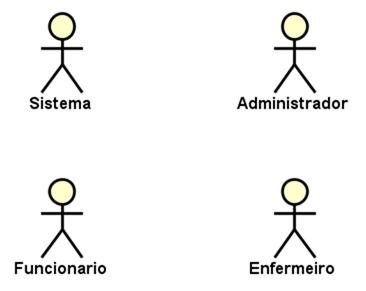
\includegraphics[width=0.55\textwidth]{figs/atores.jpg}
	\label{fig:atores}
	\fonte{Elaborado pelos autores (2025).}
\end{figure}

\section{Casos de Uso}

De acordo com \textcite{Guedes2018}, os casos de uso têm como propósito identificar os usuários de um sistema e os requisitos que orientam seu desenvolvimento, definindo “serviços, tarefas ou funcionalidades identificados como necessários ao software e que podem ser utilizados de alguma maneira pelos atores que interagem com o sistema”. Nesse contexto, a modelagem de casos de uso constitui uma etapa essencial no processo de engenharia de software, pois permite compreender, de maneira estruturada, o comportamento do sistema \textit{SeniorCareManager} e as interações estabelecidas entre os diferentes perfis de usuários.

Com base nos requisitos levantados, foram elaborados quadros que apresentam, de forma detalhada, as operações acessíveis a cada ator do sistema — Administrador, Funcionário e Enfermeiro — de acordo com suas respectivas atribuições institucionais. Essa representação possibilita uma visão clara e organizada dos fluxos de trabalho e das responsabilidades de cada perfil, assegurando que o sistema atenda simultaneamente às demandas administrativas e assistenciais do Lar São Vicente de Paulo e da APAE de Jales, promovendo maior eficiência, rastreabilidade e segurança das informações.


\subsection{Casos de Uso do Administrador}

O ator Administrador desempenha a função de maior privilégio dentro do sistema \textit{SeniorCareManager}, sendo responsável pela gestão integral e pela supervisão das atividades realizadas pelos demais usuários. As tarefas apresentadas no Quadro~\ref{quad:casos_uso_admin} são exclusivas desse ator e abrangem desde o cadastro e a manutenção de informações administrativas, como usuários, produtos e lotes, até o controle de entradas e saídas de materiais e a configuração de parâmetros do sistema. Além de executar suas próprias operações, o Administrador possui permissão para acessar, acompanhar e intervir nas ações dos demais perfis — como Funcionários e Enfermeiros — assegurando a integridade dos dados, a conformidade dos processos e a eficiência das rotinas institucionais. Dessa forma, sua atuação é essencial para garantir a governança, a rastreabilidade e a confiabilidade do sistema como um todo.

%\begin{center}
	\small
	\begin{longquadro}{|c|p{0.25\textwidth}|p{0.15\textwidth}|p{0.15\textwidth}|p{0.28\textwidth}|}
		\caption{Casos de Uso — Administrador}
		\label{quad:casos_uso_admin}\\
		\hline
		\textbf{Nº} & \textbf{Descrição do Caso de Uso} & \textbf{Entrada} & \textbf{Caso de Uso} & \textbf{Resposta} \\ \hline
		\endfirsthead
		
		\hline
		\textbf{Nº} & \textbf{Descrição do Caso de Uso} & \textbf{Entrada} & \textbf{Caso de Uso} & \textbf{Resposta} \\ \hline
		\endhead
		
		\hline
		\multicolumn{5}{r}{\textit{Continua na próxima página}} \\
		\endfoot
		
		\hline
		\multicolumn{5}{l}{\textit{Fonte: elaborado pelo autor.}}
		\endlastfoot
		
		01 & Administrador cadastra funcionário & Dados do funcionário & Cadastrar Funcionário & Mensagem: “Funcionário cadastrado com sucesso.” \\ \hline
		02 & Administrador atualiza funcionário & Dados do funcionário & Atualizar Funcionário & Mensagem: “Funcionário atualizado com sucesso.” \\ \hline
		03 & Administrador lista funcionários & — & Listar Funcionários & Retorna lista de funcionários. \\ \hline
		04 & Administrador carrega funcionário & — & Carregar Funcionário & Retorna informações do funcionário. \\ \hline
		05 & Administrador exclui funcionário & — & Excluir Funcionário & Mensagem: “Funcionário excluído com êxito.” \\ \hline
		06 & Administrador cadastra produto & Dados do produto & Cadastrar Produto & Mensagem: “Produto cadastrado com sucesso.” \\ \hline
		07 & Administrador lista produtos & — & Listar Produtos & Retorna lista de produtos. \\ \hline
		08 & Administrador atualiza produto & Dados do produto & Atualizar Produto & Mensagem: “Produto atualizado com sucesso.” \\ \hline
		09 & Administrador exclui produto & — & Excluir Produto & Mensagem: “Produto excluído com êxito.” \\ \hline
		10 & Administrador carrega produto & — & Carregar Produto & Retorna informações do produto. \\ \hline
		11 & Administrador cadastra tipo de produto & Dados do tipo de produto & Cadastrar Tipo de Produto & Mensagem: “Tipo de produto cadastrado com sucesso.” \\ \hline
		12 & Administrador lista tipos de produto & — & Listar Tipos de Produto & Retorna lista de tipos de produto. \\ \hline
		13 & Administrador atualiza tipo de produto & Dados do tipo de produto & Atualizar Tipo de Produto & Mensagem: “Tipo de produto atualizado com sucesso.” \\ \hline
		14 & Administrador exclui tipo de produto & — & Excluir Tipo de Produto & Mensagem: “Tipo de produto excluído com êxito.” \\ \hline
		15 & Administrador carrega tipo de produto & — & Carregar Tipo de Produto & Retorna informações do tipo de produto. \\ \hline
		16 & Administrador cadastra lote & Dados do lote & Cadastrar Lote & Mensagem: “Lote cadastrado com sucesso.” \\ \hline
		17 & Administrador lista lotes & — & Listar Lotes & Retorna lista de lotes. \\ \hline
		18 & Administrador atualiza lote & Dados do lote & Atualizar Lote & Mensagem: “Lote atualizado com sucesso.” \\ \hline
		19 & Administrador exclui lote & — & Excluir Lote & Mensagem: “Lote excluído com êxito.” \\ \hline
		20 & Administrador carrega lote & — & Carregar Lote & Retorna informações do lote. \\ \hline
		21 & Administrador realiza saída & Dados da saída & Realizar Saída & Mensagem: “Saída realizada com sucesso.” \\ \hline
		22 & Administrador realiza entrada & Dados da entrada & Realizar Entrada & Mensagem: “Entrada realizada com sucesso.” \\ \hline
		23 & Administrador realiza login & E-mail e senha & Login & Redireciona à página inicial (home). \\ \hline
	\end{longquadro}
%\end{center}


\subsection{Casos de Uso do Funcionário}

O ator Funcionário desempenha um papel operacional essencial no sistema \textit{SeniorCareManager}, sendo responsável pela execução das atividades cotidianas relacionadas à gestão de produtos, lotes e controle de estoque. As ações atribuídas a esse perfil estão descritas de forma detalhada no Quadro~\ref{quad:casos_uso_funcionario}, que apresenta os casos de uso aos quais o funcionário tem acesso. Esses casos englobam o cadastro, atualização, exclusão e consulta de informações pertinentes ao fluxo de materiais, além da realização de entradas e saídas de produtos. Dessa forma, o sistema assegura que o funcionário disponha de um ambiente controlado e eficiente para o desempenho de suas funções, mantendo a rastreabilidade das operações e a integridade dos dados registrados.

%\begin{center}
	\small
	\begin{longquadro}{|c|P{0.25\textwidth}|P{0.15\textwidth}|P{0.15\textwidth}|P{0.28\textwidth}|}
		\caption{Casos de Uso — Funcionário}
		\label{quad:casos_uso_funcionario}\\
		\hline
		\textbf{Nº} & \textbf{Descrição do Caso de Uso} & \textbf{Entrada} & \textbf{Caso de Uso} & \textbf{Resposta} \\
		\hline
		\endfirsthead
		
		\hline
		\textbf{Nº} & \textbf{Descrição do Caso de Uso} & \textbf{Entrada} & \textbf{Caso de Uso} & \textbf{Resposta} \\
		\hline
		\endhead
		
		\multicolumn{5}{r}{\textit{Continua na próxima página}}\\[-0.6ex]
		\noalign{\hrule height 0pt}
		\endfoot
		
		\hline
		\multicolumn{5}{l}{\textit{Fonte: elaborado pelo autor.}}\\[-0.6ex]
		\noalign{\hrule height 0pt}
		\endlastfoot
		
		01 & Funcionário realiza login & E-mail e senha & Login & Retorna tela inicial. \\ \hline
		02 & Funcionário cadastra produto & Dados do produto & Cadastrar Produto & Mensagem: ``Produto cadastrado com sucesso.'' \\ \hline
		03 & Funcionário cadastra tipo de produto & Dados do tipo de produto & Cadastrar Tipo de Produto & Mensagem: ``Tipo de produto cadastrado com sucesso.'' \\ \hline
		04 & Funcionário cadastra lote & Dados do lote & Cadastrar Lote & Mensagem: ``Lote cadastrado com sucesso.'' \\ \hline
		05 & Funcionário lista produtos & — & Listar Produtos & Retorna lista de produtos. \\ \hline
		06 & Funcionário lista tipos de produto & — & Listar Tipos de Produto & Retorna lista de tipos de produto. \\ \hline
		07 & Funcionário lista lotes & — & Listar Lotes & Retorna lista de lotes. \\ \hline
		08 & Funcionário atualiza produto & Dados do produto & Atualizar Produto & Mensagem: ``Produto atualizado com sucesso.'' \\ \hline
		09 & Funcionário atualiza tipo de produto & Dados do tipo de produto & Atualizar Tipo de Produto & Mensagem: ``Tipo de produto atualizado com sucesso.'' \\ \hline
		10 & Funcionário atualiza lote & Dados do lote & Atualizar Lote & Mensagem: ``Lote atualizado com sucesso.'' \\ \hline
		11 & Funcionário exclui produto & — & Excluir Produto & Mensagem: ``Produto excluído com êxito.'' \\ \hline
		12 & Funcionário exclui tipo de produto & — & Excluir Tipo de Produto & Mensagem: ``Tipo de produto excluído com êxito.'' \\ \hline
		13 & Funcionário exclui lote & — & Excluir Lote & Mensagem: ``Lote excluído com êxito.'' \\ \hline
		14 & Funcionário carrega produto & ID do produto & Carregar Produto & Retorna informações do produto. \\ \hline
		15 & Funcionário carrega tipo de produto & ID do tipo de produto & Carregar Tipo de Produto & Retorna informações do tipo de produto. \\ \hline
		16 & Funcionário carrega lote & ID do lote & Carregar Lote & Retorna informações do lote. \\ \hline
		17 & Funcionário realiza entrada & Dados da entrada & Realizar Entrada & Mensagem: ``Entrada realizada com sucesso.'' \\ \hline
		18 & Funcionário realiza saída & Dados da saída & Realizar Saída & Mensagem: ``Saída realizada com sucesso.'' \\
		% não coloque \hline na última linha da ÚLTIMA página
	\end{longquadro}
%\end{center}


\subsection{Casos de Uso do Enfermeiro}

O ator Enfermeiro possui atribuições voltadas ao acompanhamento assistencial e ao gerenciamento das informações clínicas dos residentes no sistema \textit{SeniorCareManager}. Conforme demonstrado no Quadro~\ref{quad:casos_uso_enfermeiro}, os casos de uso associados a esse perfil abrangem o cadastramento, atualização e exclusão de dados referentes a idosos, carteiras de vacinação, vacinas aplicadas e agendamentos. Além disso, o enfermeiro tem acesso a funcionalidades que permitem o controle do histórico vacinal e o monitoramento da saúde dos residentes, favorecendo uma gestão mais segura e organizada da assistência prestada. Dessa forma, as operações disponíveis ao enfermeiro contribuem diretamente para a qualidade do cuidado e para a integração das informações entre os diferentes setores da instituição.

%\begin{center}
	\small
	\begin{longquadro}{|c|P{0.25\textwidth}|P{0.15\textwidth}|P{0.15\textwidth}|P{0.28\textwidth}|}
		\caption{Casos de Uso — Enfermeiro}
		\label{quad:casos_uso_enfermeiro}\\
		\hline
		\textbf{Nº} & \textbf{Descrição do Caso de Uso} & \textbf{Entrada} & \textbf{Caso de Uso} & \textbf{Resposta} \\
		\hline
		\endfirsthead
		
		\hline
		\textbf{Nº} & \textbf{Descrição do Caso de Uso} & \textbf{Entrada} & \textbf{Caso de Uso} & \textbf{Resposta} \\
		\hline
		\endhead
		
		\multicolumn{5}{r}{\textit{Continua na próxima página}}\\[-0.6ex]
		\noalign{\hrule height 0pt}
		\endfoot
		
		\hline
		\multicolumn{5}{l}{\textit{Fonte: elaborado pelo autor.}}\\[-0.6ex]
		\noalign{\hrule height 0pt}
		\endlastfoot
		
		01 & Pessoa cadastra carteira de vacinação & Dados da carteira de vacinação & Cadastrar Carteira de Vacinação & Mensagem 01 \\ \hline
		02 & Enfermeiro cadastra dados da carteira de vacinação & Dados da carteira de vacinação & Cadastrar Dados da Carteira de Vacinação & Mensagem 02 \\ \hline
		03 & Enfermeiro lista idosos & — & Listar Idosos & Mensagem 03 \\ \hline
		04 & Enfermeiro cadastra idoso & Dados do idoso & Cadastrar Idoso & Mensagem 04 \\ \hline
		05 & Enfermeiro edita idoso & ID e dados do idoso & Editar Idoso & Mensagem 05 \\ \hline
		06 & Enfermeiro exclui idoso & ID do idoso & Excluir Idoso & Mensagem 06 \\ \hline
		07 & Enfermeiro lista agendamentos de vacina & — & Listar Agendamento de Vacina & Mensagem 07 \\ \hline
		08 & Enfermeiro cadastra agendamento de vacina & Dados do agendamento & Cadastrar Agendamento de Vacina & Mensagem 08 \\ \hline
		09 & Enfermeiro edita dados do agendamento & ID e dados do agendamento & Editar Dados do Agendamento & Mensagem 09 \\ \hline
		10 & Enfermeiro exclui idosos que não desejam vacinação & ID do idoso & Excluir Idoso Não Vacinado & Mensagem 10 \\ \hline
		11 & Administrador cadastra lote de vacina & Dados do lote de vacina & Cadastrar Lote de Vacina & Mensagem 11 \\ \hline
		12 & Administrador lista lotes de vacina & — & Listar Lotes de Vacina & Mensagem 12 \\ \hline
		13 & Administrador exclui lote de vacina & ID do lote de vacina & Excluir Lote de Vacina & Mensagem 13 \\ \hline
		14 & Administrador edita lote de vacina & ID e dados do lote & Editar Lote de Vacina & Mensagem 14 \\ \hline
		15 & Administrador cadastra vacina aplicada & Dados da vacina aplicada & Cadastrar Vacina Aplicada & Mensagem 15 \\ \hline
		16 & Administrador exclui vacina aplicada & ID da vacina aplicada & Excluir Vacina Aplicada & Mensagem 16 \\ \hline
		17 & Administrador edita vacina aplicada & ID e dados da vacina aplicada & Editar Vacina Aplicada & Mensagem 17 \\ \hline
		18 & Administrador lista vacinas aplicadas & — & Listar Vacinas Aplicadas & Mensagem 18 \\ \hline
		19 & Administrador lista carteiras de vacinação & — & Listar Carteiras de Vacinação & Mensagem 19 \\ \hline
		20 & Administrador lista dados da carteira de vacinação & ID da carteira & Listar Dados da Carteira de Vacinação & Mensagem 20 \\ \hline
		21 & Administrador edita dados da carteira de vacinação & ID e dados da carteira & Editar Dados da Carteira de Vacinação & Mensagem 21 \\ \hline
		22 & Administrador exclui dados da carteira de vacinação & ID da carteira & Excluir Dados da Carteira de Vacinação & Mensagem 22 \\ \hline
		23 & Administrador exclui carteira de vacinação & ID da carteira & Excluir Carteira de Vacinação & Mensagem 23 \\
		% não coloque \hline na última linha da ÚLTIMA página
	\end{longquadro}
%\end{center}

\section{Diagrama de Casos de Uso}

\textcite{Guedes2018} descreve o \textit{diagrama de casos de uso} como uma representação do sistema a partir da perspectiva do usuário, cujo objetivo é apresentar, de forma geral, as funcionalidades que o sistema deve oferecer ao usuário. Além disso, Guedes (2018) destaca que esse diagrama é uma ferramenta essencial para identificar e compreender os requisitos do sistema, auxiliando na especificação, visualização e documentação das características, funções e serviços que o sistema deve proporcionar.

O diagrama de caso de uso geral fornece uma visão abrangente das diversas interações que cada usuário pode realizar no sistema. Essa representação é especialmente valiosa para obter uma compreensão global das funcionalidades disponíveis para cada ator envolvido. Nas Figuras~\ref{fig:UCGAdministrador}, \ref{fig:UCGEnfermeiro} e \ref{fig:UCGFuncionario}, são apresentados os casos de uso gerais, destacando as ações que cada ator pode executar no sistema. Essa abordagem oferece uma visão consolidada das capacidades do sistema, facilitando a compreensão das funcionalidades disponíveis para cada usuário.

O diagrama de caso de uso geral apresentado na Figura~\ref{fig:UCGAdministrador}
descreve todas as interações possíveis entre o ator Administrador e o
Sistema, evidenciando as funcionalidades de gestão relacionadas aos
usuários do sistema e aos idosos cadastrados. Esse diagrama oferece uma visão
abrangente das operações administrativas, permitindo compreender como o ator
atua na manutenção das informações essenciais para o funcionamento adequado do
ambiente institucional.

Na visão do administrador, o processo tem início com o caso de uso
\textit{Realizar Login}, que habilita o acesso às funcionalidades seguintes.
Após a autenticação, o administrador pode executar atividades referentes à
gestão de outros administradores, funcionários e idosos. Entre essas
funcionalidades destacam-se: \textit{Cadastrar Administrador},
\textit{Atualizar Administrador}, \textit{Listar Administrador},
\textit{Excluir Administrador} e \textit{Validar Administrador}. Essas ações
representam o controle hierárquico do sistema, permitindo que o administrador
tenha domínio sobre os perfis de acesso e suas permissões.

O diagrama também evidencia as operações de gerenciamento de idosos, tais como
\textit{Cadastrar Idoso}, \textit{Atualizar Idoso}, \textit{Listar Idoso},
\textit{Excluir Idoso}, \textit{Validar Idoso} e \textit{Carregar Idoso}. Todas
essas funcionalidades são essenciais para manter atualizadas as informações
clínicas e cadastrais dos residentes, garantindo consistência e rastreabilidade
dos dados.

Além disso, o administrador possui acesso à gestão de funcionários por meio dos
casos de uso \textit{Cadastrar Funcionário}, \textit{Atualizar Funcionário},
\textit{Listar Funcionário}, \textit{Excluir Funcionário}, \textit{Validar
	Funcionário} e \textit{Carregar Funcionário}. Cada um desses casos está
relacionado ao fluxo de manutenção dos colaboradores que operam o sistema,
permitindo que o administrador assegure controle organizacional e operacional.

\begin{figure}[H]
	%\centering
	\caption{Diagrama de Caso de Uso Geral - Administrador}
	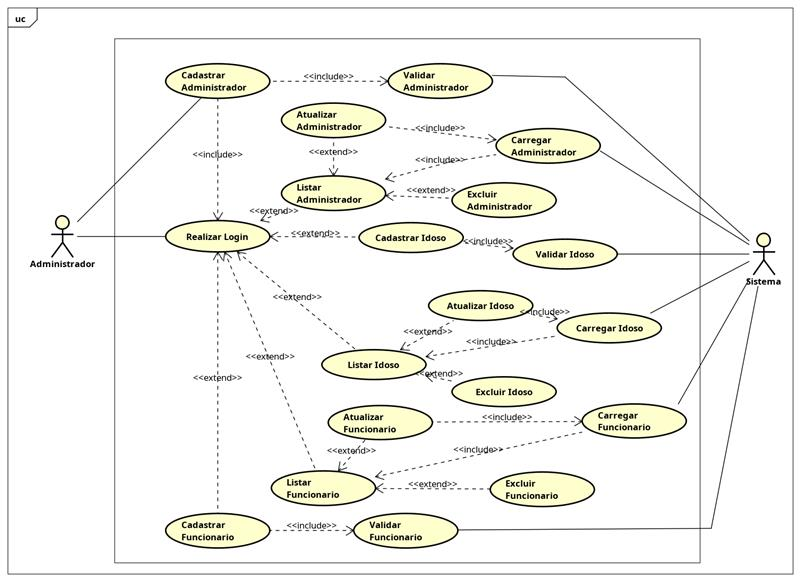
\includegraphics[width=1\linewidth]{figs/UCGeral_Administrador.jpg}
	\label{fig:UCGAdministrador}
	\fonte{Elaborada pelos autores.}
\end{figure}

As relações \textit{include} e \textit{extend} presentes no diagrama demonstram
a modularidade e a reutilização de comportamentos, reforçando a lógica de que
algumas operações dependem de ações anteriores — como a necessidade de carregar
dados antes de validá-los — ou podem ser especializadas a partir de um fluxo
principal. Dessa forma, o diagrama sintetiza a complexidade e a amplitude das
funções administrativas, oferecendo uma visão estruturada do papel central do
Administrador no gerenciamento do sistema.

Na Figura~\ref{fig:UCGEnfermeiro}, apresenta-se o diagrama de casos de uso geral na perspectiva do ator \textit{Enfermeiro}. Conforme exposto por \textcite{Guedes2018}, o diagrama de casos de uso tem como objetivo representar as funcionalidades do sistema a partir do ponto de vista do usuário, destacando as interações possíveis entre o ator e o sistema. Nesse contexto, o \textit{Enfermeiro} é o profissional que utiliza o sistema para registrar e acompanhar as informações clínicas dos idosos assistidos.

Inicialmente, o \textit{Enfermeiro} realiza o caso de uso \textit{Realizar Login}, que lhe concede acesso às funcionalidades internas do sistema. A partir disso, ele pode executar o caso de uso \textit{Listar Idosos}, que permite localizar o idoso desejado e, em seguida, acionar o caso de uso central \textit{Abrir Prontuário}. Esse caso de uso funciona como eixo principal do diagrama, pois concentra a maior parte das interações clínicas realizadas pelo profissional de enfermagem.

\begin{figure}[H]
	%\centering
	\caption{Diagrama de Caso de Uso Geral - Enfermeiro}
	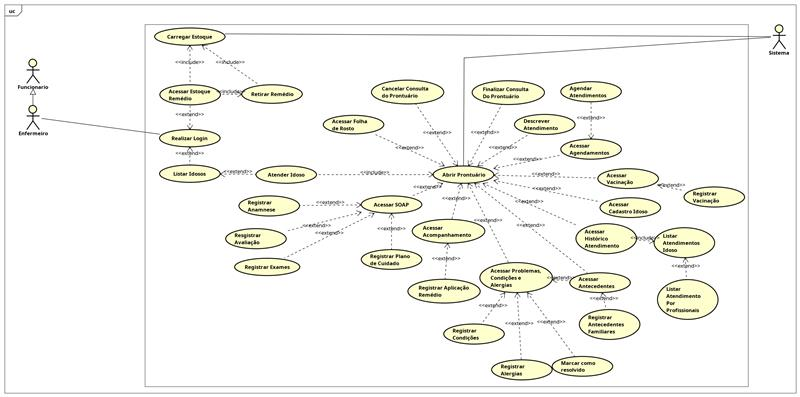
\includegraphics[width=1\linewidth]{figs/UCGeral_Enfermeiro.jpg}
	\label{fig:UCGEnfermeiro}
	\fonte{Elaborada pelos autores.}
\end{figure}

Uma vez com o prontuário aberto, o \textit{Enfermeiro} pode acessar diferentes seções e registros, tais como \textit{Acessar SOAP}, \textit{Acessar Acompanhamento}, \textit{Acessar Cadastro Idoso}, \textit{Acessar Histórico de Atendimento} e \textit{Acessar Problemas, Condições e Alergias}. Cada uma dessas funcionalidades dá suporte a ações específicas do cuidado, permitindo ao ator consultar e atualizar informações relevantes sobre o estado de saúde do idoso.

O diagrama também evidencia casos de uso voltados ao registro de informações assistenciais, como \textit{Registrar Anamnese}, \textit{Registrar Avaliação}, \textit{Registrar Exames}, \textit{Registrar Plano de Cuidado}, \textit{Registrar Aplicação de Remédio}, \textit{Registrar Condições}, \textit{Registrar Alergias} e \textit{Registrar Antecedentes Familiares}. Tais casos de uso estão associados ao processo de documentação sistemática da assistência, garantindo rastreabilidade e continuidade do cuidado. Além disso, o \textit{Enfermeiro} pode marcar problemas como resolvidos, bem como acessar e registrar informações relacionadas a atendimentos, agendamentos e vacinação, assegurando uma visão longitudinal do acompanhamento clínico.

Dessa forma, o diagrama de caso de uso geral na visão do \textit{Enfermeiro} apresenta um conjunto abrangente de funcionalidades orientadas à prática assistencial, reforçando o papel central desse profissional na utilização do sistema para registro, monitoramento e tomada de decisão em relação à saúde dos idosos.

O diagrama de caso de uso apresentado na Figura~\ref{fig:UCGFuncionario} ilustra, de forma ampliada, todas as interações possíveis entre o ator Funcionário e o Sistema no contexto do gerenciamento do prontuário eletrônico do idoso. A figura representa um panorama geral das funcionalidades acessíveis ao funcionário, evidenciando tanto os fluxos diretamente iniciados por ele quanto aqueles acionados como extensões ou inclusões decorrentes de outras operações.

Inicialmente, o funcionário pode listar idosos e, a partir dessa ação, proceder ao atendimento do idoso. O atendimento dá origem à operação de abrir prontuário, considerada central no diagrama, pois dela se ramificam diversas funcionalidades essenciais ao registro e acompanhamento clínico. Entre essas funcionalidades, destacam-se: Acessar SOAP, Registrar Anamnese, Registrar Avaliação, Registrar Exames, Registrar Plano de Cuidado, Registrar Aplicação de Remédio, Registrar Condições e Registrar Alergias. Todas essas operações estendem o acesso ao módulo SOAP, reforçando a estrutura lógica do prontuário clínico.

\begin{figure}[H]
	%\centering
	\caption{Diagrama de Caso de Uso Geral - Profissional}
	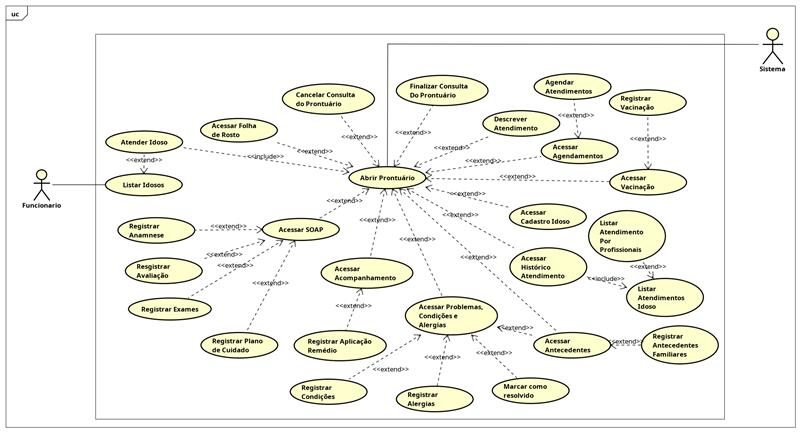
\includegraphics[width=1\linewidth]{figs/UCGeral_Funcionario.jpg}
	\label{fig:UCGFuncionario}
	\fonte{Elaborada pelos autores.}
\end{figure}

Além disso, o funcionário também interage com funções de gestão do atendimento, como Acessar Acompanhamento, Acessar Problemas, Condições e Alergias, Acessar Histórico de Atendimento, Acessar Antecedentes, Acessar Antecedentes Familiares, Acessar Cadastro do Idoso e Acessar Agendamentos. O diagrama também contempla ações administrativas relacionadas ao fluxo de atendimento, como Cancelar Consulta do Prontuário, Finalizar Consulta do Prontuário e Marcar como Resolvido.

A modelagem demonstra ainda a interação indireta entre o funcionário e o sistema na emissão de notificações, descrição de atendimentos e registro de vacinação, ações que surgem como extensões específicas do processo principal. Ao organizar visualmente esses relacionamentos, o diagrama fornece uma visão clara e sistematizada das responsabilidades do ator e do comportamento esperado do sistema, facilitando tanto o entendimento quanto a documentação dos requisitos funcionais associados ao módulo de prontuário eletrônico.

\section{Diagrama de Casos de Uso - Individuais}

De acordo com \textcite{Guedes2018}, o diagrama de caso de uso é uma representação gráfica das interações entre um sistema e seus usuários. Seu principal objetivo é descrever, de maneira simples e intuitiva, as funcionalidades que o sistema oferece, facilitando o entendimento tanto para os desenvolvedores quanto para os usuários. Além disso, esse tipo de diagrama proporciona uma visão geral do funcionamento do sistema, destacando as interações com os diferentes tipos de usuários que podem acessá-lo.

Nos tópicos a seguir, serão apresentados alguns dos casos de uso do sistema, contemplando funcionalidades específicas de um CRUD do SOAP do prontuário do atendido pela instituição.

O método SOAP é uma forma estruturada de registro utilizada em prontuários clínicos para organizar as informações do paciente de maneira clara, objetiva e padronizada. A sigla SOAP corresponde aos termos \textbf{S}ubjetivo, \textbf{O}bjetivo, \textbf{A}valiação e \textbf{P}lano. Na seção Subjetiva, são descritas as queixas, percepções e sentimentos relatados pelo paciente; na Objetiva, registram-se sinais clínicos observáveis, dados mensuráveis e resultados de exames físicos ou complementares. A Avaliação reúne a interpretação profissional dessas informações, incluindo hipóteses diagnósticas e justificativas clínicas; por fim, o Plano define as condutas a serem adotadas, como tratamentos, prescrições, exames adicionais ou orientações. Dessa forma, o SOAP contribui para a organização do cuidado, favorecendo a continuidade assistencial e a comunicação entre os profissionais de saúde.
 
Esses casos de uso foram elaborados com o objetivo de proporcionar uma compreensão mais aprofundada sobre o funcionamento do sistema, ilustrando as interações entre os usuários e o sistema em diferentes áreas de gerenciamento.

A descrição de cada caso de uso visa facilitar a visualização do fluxo de atividades e das tarefas que podem ser executadas no sistema, além de evidenciar a lógica envolvida em cada operação.

\subsection{Caso de Uso Individual - Cadastro de SOAP}

Os casos de uso apresentados nesta seção foram elaborados a partir do documento-base fornecido pelo usuário, descrevendo de forma detalhada o fluxo de interação entre o ator \textbf{Funcionário} e o \textbf{Sistema} no contexto do prontuário eletrônico do idoso, abrangendo registros clínicos, avaliações e procedimentos. 

A Figura~\ref{fig:caso_uso_prontuario} apresenta o diagrama de caso de uso que representa as principais interações entre os atores \textbf{Funcionário}, \textbf{Enfermeiro} e o \textbf{Sistema} no contexto das atividades relacionadas ao prontuário eletrônico do idoso. O diagrama evidencia o fluxo geral de ações necessárias para o atendimento, incluindo listagem e seleção do idoso, abertura do prontuário e acesso ao modelo SOAP, bem como os casos de uso estendidos envolvendo o registro de anamnese, avaliação, exames e plano de cuidado. Essa representação permite visualizar de forma clara e organizada a estrutura funcional do módulo de prontuário, destacando como cada ação se relaciona e se integra ao processo assistencial.

\begin{figure}[H]
	%\centering
	\caption{Diagrama de Caso: Prontuário SOAP}
	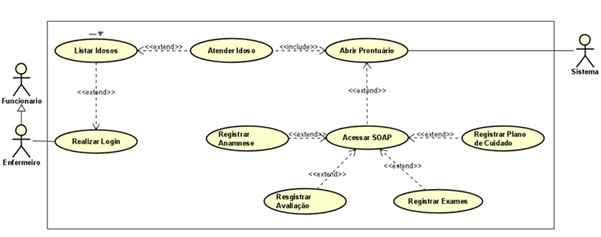
\includegraphics[width=\linewidth]{figs/UC_Soap.jpg}
	\label{fig:caso_uso_prontuario}
	\fonte{Elaborada pelos autores.}
\end{figure}

Cada caso de uso foi estruturado seguindo um padrão que inclui resumo, pré-condições, pós-condições, cenário principal e possíveis variações alternativas ou de exceção. No caso específico relacionado ao acesso ao modelo SOAP, destaca-se que sua finalidade é permitir ao funcionário visualizar informações clínicas organizadas nos componentes Subjetivo, Objetivo, Avaliação e Plano, fundamentais para assegurar a continuidade e a qualidade do atendimento.

No Quadro \ref{quad:acessarSOAP} tem-se o fluxo para o funcionário acessar o SOAP de um idoso assistido pela entidade.

\begin{quadro}[H]
	\centering
	\caption{UC: Acessar SOAP}
	\begin{tabular}{|p{5cm}|p{10cm}|}
		\hline
		\textbf{Ator Principal} & Funcionário \\ \hline
		
		\textbf{Atores Secundários} & Sistema \\ \hline
		
		\textbf{Resumo} & Descreve as etapas para o funcionário acessar as informações do prontuário SOAP de um idoso. \\ \hline
		
		\textbf{Pré-condições} & Atender um idoso, abrir o prontuário e estar logado no sistema. \\ \hline
		
		\textbf{Pós-condições} & -- \\ \hline
		
		\textbf{Cenário Principal} &
		\textbf{Ações do Ator:} \newline
		1. Clica em “Acessar SOAP”. \newline
		\textbf{Ações do Sistema:} \newline
		2. Exibe os campos do SOAP (subjetivo, objetivo, avaliação e plano). \\ \hline
		
		\textbf{Restrições e Validações} & O idoso deve estar cadastrado. \\ \hline
		
		\textbf{Cenário Alternativo} & Não há. \\ \hline
		
		\textbf{Cenário de Exceção} & Não há. \\ \hline
	\end{tabular}
	\label{quad:acessarSOAP}
	\fonte{Elaborada pelos autores.}
\end{quadro}

No Quadro \ref{quad:regAnamnese} trata-se do registro da anamnese, etapa fundamental na coleta de informações subjetivas sobre o estado de saúde do idoso.

\begin{quadro}[H]
	\centering
	\caption{UC: Registrar Anamnese}
	\begin{tabular}{|p{5cm}|p{10cm}|}
		\hline
		\textbf{Ator Principal} & Funcionário \\ \hline
		
		\textbf{Atores Secundários} & Sistema \\ \hline
		
		\textbf{Resumo} & Descreve as etapas para preenchimento da anamnese de um idoso. \\ \hline
		
		\textbf{Pré-condições} & Atender um idoso, abrir o prontuário e estar logado. \\ \hline
		
		\textbf{Pós-condições} & -- \\ \hline
		
		\textbf{Cenário Principal} &
		1. Funcionário acessa o SOAP. \newline
		2. Sistema exibe os campos SOAP. \newline
		3. Funcionário seleciona “Registrar Anamnese”. \newline
		4. Sistema mostra o formulário. \newline
		5. Funcionário preenche as informações. \newline
		7. Sistema valida e salva os dados. \\ \hline
		
		\textbf{Restrições e Validações} & Idoso deve estar cadastrado. \\ \hline
		
		\textbf{Cenário Alternativo} & 
		Dados Inválidos: \newline
		1. Sistema avisa sobre dados inválidos. \newline
		2. Pedido é recusado. \\ \hline
		
		\textbf{Cenário de Exceção} & Não há. \\ \hline
	\end{tabular}
	\label{quad:regAnamnese}
	\fonte{Elaborada pelos autores.}
\end{quadro}

Para o caso de uso Registrar Avaliação (Quadro \ref{quad:regAvaliacao}) descreve-se a etapa de avaliação clínica, contemplando análise subjetiva e objetiva, com inserção de códigos CIAP2 e CID-10.

\begin{quadro}[H]
	%\centering
	\caption{UC: Registrar Avaliação}
	\begin{tabular}{|p{5cm}|p{10cm}|}
		\hline
		\textbf{Ator Principal} & Funcionário \\ \hline
		
		\textbf{Atores Secundários} & Sistema \\ \hline
		
		\textbf{Resumo} & Descreve as etapas de avaliação clínica baseada nos blocos Subjetivo e Objetivo. \\ \hline
		
		\textbf{Pré-condições} & Atendimento ativo, prontuário aberto e login efetuado. \\ \hline
		
		\textbf{Pós-condições} & -- \\ \hline
		
		\textbf{Cenário Principal} &
		1. Acessar SOAP. \newline
		2. Sistema exibe campos. \newline
		3. Funcionário informa CIAP2, CID-10 e observações. \newline
		4. Sistema valida. \newline
		5. Sistema salva. \\ \hline
		
		\textbf{Restrições e Validações} &
		1. Idoso deve estar cadastrado. \newline
		2. Informar pelo menos um código (CIAP2 ou CID-10). \\ \hline
		
		\textbf{Cenário Alternativo} & Não há. \\ \hline
		
		\textbf{Cenário de Exceção} & Não há. \\ \hline
	\end{tabular}
	\label{quad:regAvaliacao}
	\fonte{Elaborada pelos autores.}
\end{quadro}

No caso de uso Registrar Exames (Quadro \ref{quad:regExame}) demonstra-se o registro de exames contempla campos estruturados para aferições clínicas rotineiras, como antropometria, sinais vitais e glicemia.

\begin{quadro}[H]
	%\centering
	\caption{UC: Registrar Exames}
	\begin{tabular}{|p{5cm}|p{10cm}|}
		\hline
		\textbf{Ator Principal} & Funcionário \\ \hline
		
		\textbf{Atores Secundários} & Sistema \\ \hline
		
		\textbf{Resumo} & Descreve o processo de registro de exames realizados ou solicitados para o idoso, incluindo informações clínicas e anexação de resultados. \\ \hline
		
		\textbf{Pré-condições} & Prontuário aberto, atendimento ativo e usuário logado. \\ \hline
		
		\textbf{Pós-condições} & O exame é registrado e armazenado no prontuário eletrônico. \\ \hline
		
		\textbf{Cenário Principal} &
		1. Acessar SOAP. \newline
		2. Sistema exibe os campos disponíveis. \newline
		3. Funcionário seleciona “Registrar Exames”. \newline
		4. Sistema apresenta o formulário de registro de exames. \newline
		5. Funcionário informa tipo de exame, data, observações e anexa arquivo (opcional). \newline
		6. Sistema valida as informações. \newline
		7. Sistema salva o registro no prontuário. \\ \hline
		
		\textbf{Restrições e Validações} &
		1. O idoso deve estar cadastrado. \newline
		2. Informações obrigatórias devem ser preenchidas (tipo e data do exame). \\ \hline
		
		\textbf{Cenário Alternativo – Dados Inválidos} &
		1. Sistema identifica dados inconsistentes ou campos obrigatórios vazios. \newline
		2. Sistema informa o erro ao usuário. \newline
		3. Funcionário revisa e corrige os dados. \\ \hline
		
		\textbf{Cenário de Exceção} & Falha ao anexar o arquivo ou indisponibilidade temporária do sistema. \\ \hline
	\end{tabular}
	\label{quad:regExame}
	\fonte{Elaborada pelos autores.}
\end{quadro}

No caso de uso Plano de Cuidado (Quadro \ref{quad:planoCuidado}) tem-se o eixo central do acompanhamento de saúde, reunindo prescrições, orientações, encaminhamentos e lembretes clínicos.

\begin{quadro}[H]
%	\centering
	\caption{UC: Registrar Plano de Cuidado}
	\begin{tabular}{|p{5cm}|p{10cm}|}
		\hline
		\textbf{Ator Principal} & Funcionário \\ \hline
		
		\textbf{Atores Secundários} & Sistema \\ \hline
		
		\textbf{Resumo} & Descreve o processo de criação e atualização do plano de cuidado do idoso, incluindo metas, prescrições e condutas assistenciais. \\ \hline
		
		\textbf{Pré-condições} & Prontuário aberto, atendimento ativo e usuário autenticado. \\ \hline
		
		\textbf{Pós-condições} & O plano de cuidado é registrado e disponibilizado para consulta. \\ \hline
		
		\textbf{Cenário Principal} &
		1. Acessar SOAP. \newline
		2. Sistema exibe os campos disponíveis. \newline
		3. Funcionário seleciona “Registrar Plano de Cuidado”. \newline
		4. Sistema apresenta o formulário de plano de cuidado. \newline
		5. Funcionário preenche diagnósticos, intervenções e metas assistenciais. \newline
		6. Sistema valida as informações. \newline
		7. Sistema salva o plano de cuidado no prontuário eletrônico. \\ \hline
		
		\textbf{Restrições e Validações} &
		1. O idoso deve estar cadastrado. \newline
		2. O plano deve conter ao menos uma intervenção ou diagnóstico. \\ \hline
		
		\textbf{Cenário Alternativo – Dados Insuficientes} &
		1. Sistema identifica ausência de dados essenciais. \newline
		2. Sistema notifica o usuário sobre o preenchimento obrigatório. \newline
		3. Funcionário ajusta o formulário. \\ \hline
		
		\textbf{Cenário de Exceção} & Não há. \\ \hline
	\end{tabular}
	\label{quad:planoCuidado}
	\fonte{Elaborada pelos autores.}
\end{quadro}


\section{Diagrama de Sequência}

Os diagramas de sequência desempenham um papel essencial na modelagem de sistemas, pois representam de maneira clara a ordem cronológica das interações entre objetos, serviços, camadas e atores envolvidos na execução de um determinado comportamento.

Segundo \textcite{Sommerville2018ES10}, esse tipo de diagrama destaca o fluxo temporal das mensagens, revelando como os componentes colaboram para realizar uma operação. Da mesma forma, \textcite{Pressman2011ES7} reforça que diagramas de sequência são ferramentas fundamentais para compreender o comportamento dinâmico do software, permitindo visualizar a troca de mensagens e o encadeamento lógico das ações.

No contexto do sistema analisado, os diagramas de sequência foram desenvolvidos para representar o funcionamento completo das operações de manutenção de dados sobre \textit{resident relatives} (parentes ou associados do residente). As representações incluem as operações de \textbf{listar}, \textbf{cadastrar}, \textbf{editar} e \textbf{remover}, conforme detalhadas no documento base fornecido pelo usuário:contentReference[oaicite:0]{index=0}. Cada diagrama descreve a colaboração entre a WebApp, os controladores, os serviços de domínio, os repositórios e o banco de dados, evidenciando a utilização do padrão DTO (\textit{Data Transfer Object}), padrão amplamente recomendado por \textcite{Guedes2018} para garantir organização, modularidade e independência de camadas.

A seguir, apresenta-se a descrição detalhada de cada diagrama, acompanhada das
Figuras~\ref{fig:seq_listar_residentrelative},
\ref{fig:seq_cadastrar_residentrelative},
\ref{fig:seq_editar_residentrelative} e
\ref{fig:seq_remover_residentrelative}, que ilustram, respectivamente, os
processos de listagem, cadastro, edição e remoção de parentes de residentes.

\subsection{Diagrama de Sequência: Listar Parente de Residente}

O diagrama de sequência de listagem (Figura~\ref{fig:seq_listar_residentrelative})
descreve o fluxo necessário para recuperar as informações de um parente
associado ao residente. O processo inicia-se com o usuário acessando a página
correspondente na WebApp, que, por sua vez, envia uma requisição HTTP ao
\textit{controller}. Este repassa o processamento para a camada de serviço, que
consulta o repositório e o banco de dados. Após recuperar a entidade, ocorre a
criação de um DTO, que retorna até o usuário final por meio de uma resposta HTTP
(\texttt{200 OK}). Esse fluxo reflete a arquitetura em camadas descrita por
\textcite{Sommerville2018ES10}, reforçando a separação entre lógica de negócio, acesso
a dados e apresentação.

\begin{figure}[H]
	%\centering
	\caption{Diagrama de sequência para listagem de parente de residente.}
	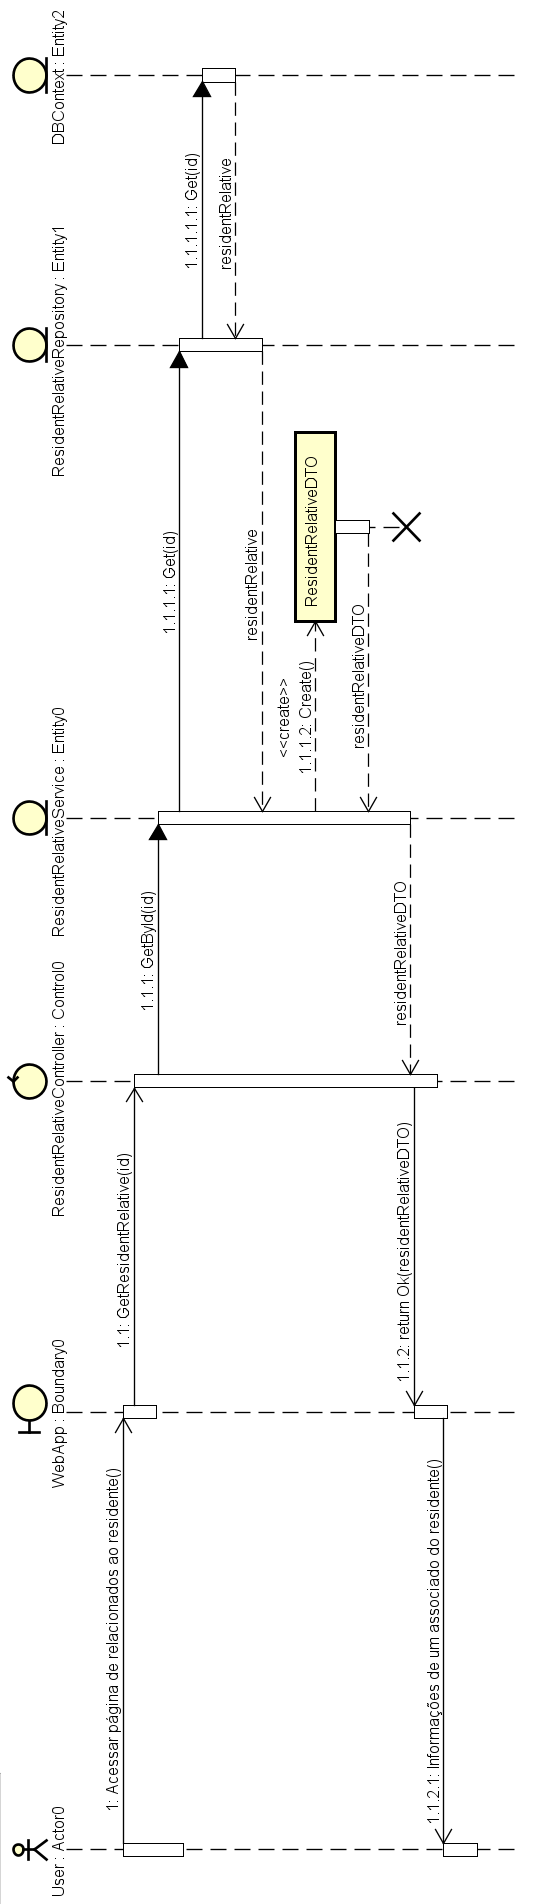
\includegraphics[width=0.4\textwidth]{figs/ResidentRelative_Listar.png}
	\label{fig:seq_listar_residentrelative}
	\fonte{Elaborada pelos autores.}
\end{figure}

\subsection{Diagrama de Sequência: Cadastrar Parente de Residente}

O cadastro de um novo parente de residente é representado na
Figura~\ref{fig:seq_cadastrar_residentrelative}. O fluxo inicia-se com a
submissão de um formulário na WebApp, contendo os dados inseridos pelo usuário.
A aplicação encaminha essas informações ao \textit{controller}, que cria um DTO e
o repassa para a camada de serviço. A entidade correspondente é instanciada,
validada e persistida no banco de dados por meio do repositório. Após a
inserção, os dados são retornados como um DTO atualizado, incluindo o novo
identificador. Essa dinâmica representa fielmente a abordagem orientada a
objetos recomendada por \textcite{Guedes2018}, na qual cada camada desempenha um papel específico e bem definido.

\begin{figure}[H]
	%\centering
	\caption{Diagrama de sequência para cadastro de parente de residente.}
	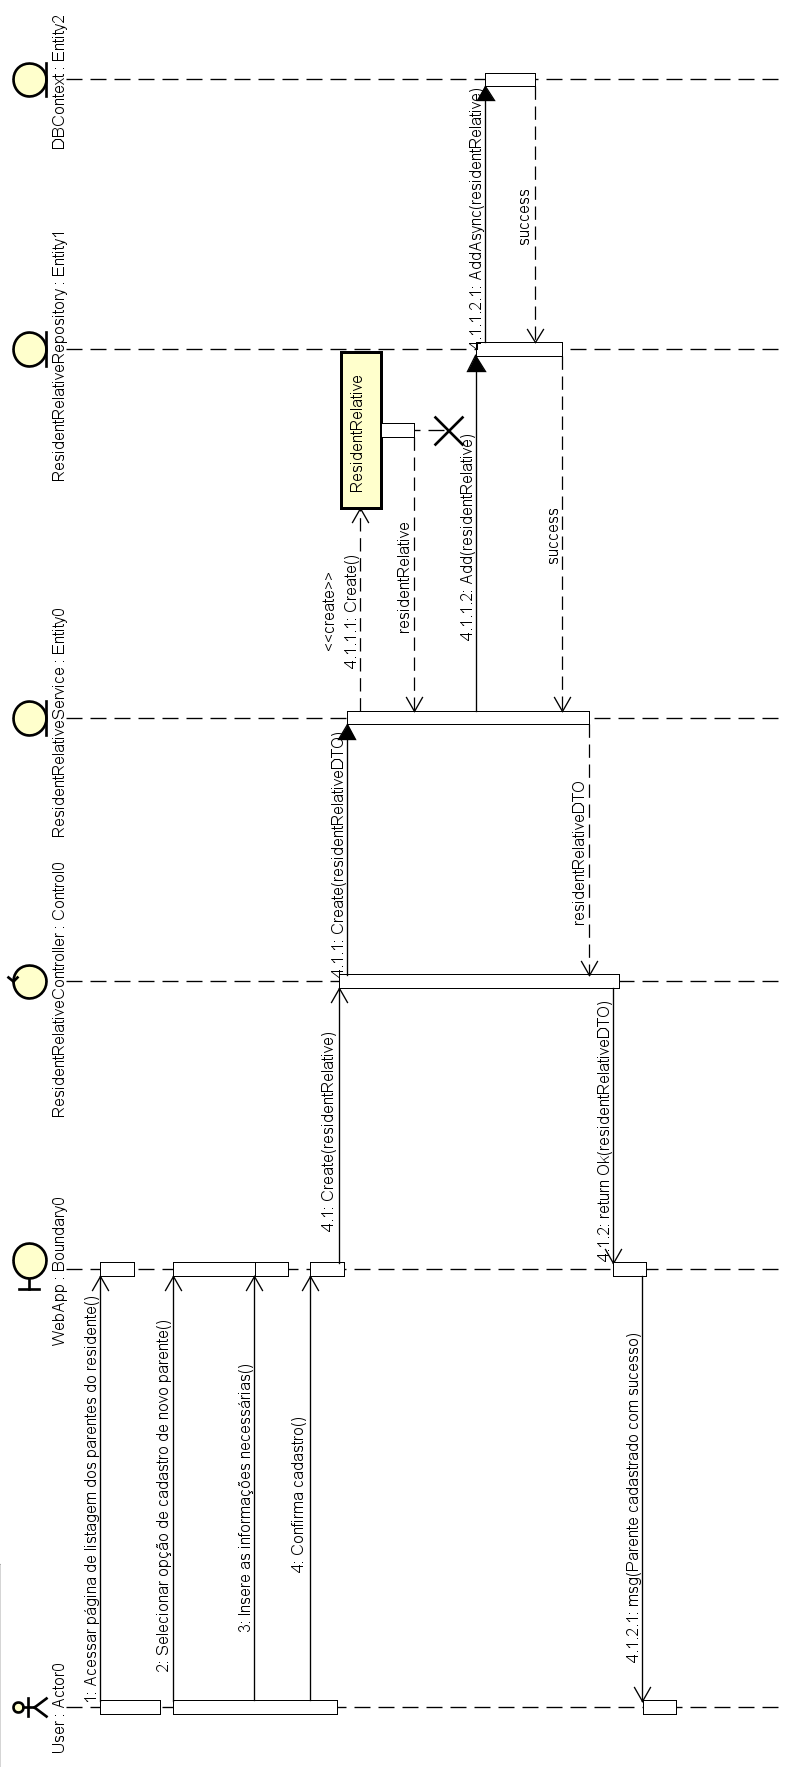
\includegraphics[width=0.45\textwidth]{figs/ResidentRelative_Cadastrar.png}
	\label{fig:seq_cadastrar_residentrelative}
	\fonte{Elaborada pelos autores.}
\end{figure}

\subsection{Diagrama de Sequência: Editar Parente de Residente}

A edição de dados de um parente de residente é apresentada na
Figura~\ref{fig:seq_editar_residentrelative}. O processo inicia-se com o acesso
à página de listagem, seguido da seleção do parente a ser alterado. O sistema
exibe o formulário de edição com os dados atuais e, após a submissão das novas
informações, o \textit{controller} encaminha a requisição à camada de serviço,
que atualiza a entidade no repositório e persiste as alterações no banco de
dados. Ao final, um DTO atualizado é retornado à interface, permitindo ao
usuário visualizar a confirmação do sucesso da operação. Assim como nos demais
diagramas, observa-se o uso consistente do padrão DTO, o que, segundo
\textcite{Pressman2011ES7}, contribui para a flexibilidade e manutenção do sistema.

\begin{figure}[H]
	%\centering
	\caption{Diagrama de sequência para edição de parente de residente.}
	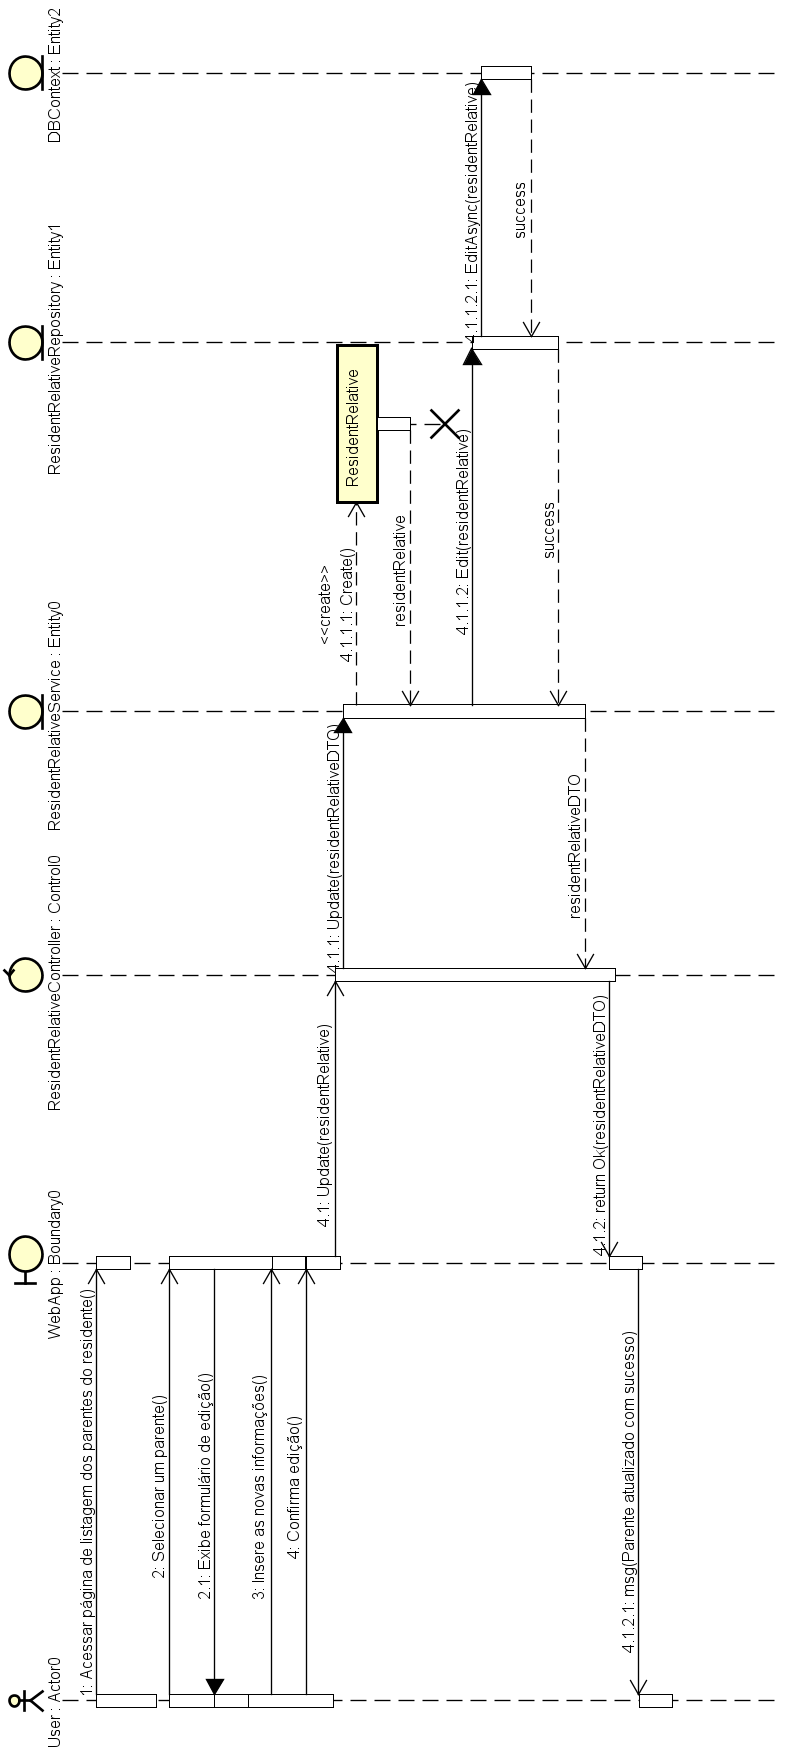
\includegraphics[width=0.45\textwidth]{figs/ResidentRelative_Editar.png}
	\label{fig:seq_editar_residentrelative}
	\fonte{Elaborada pelos autores.}
\end{figure}

\subsection{Diagrama de Sequência: Remover Parente de Residente}

A operação de remoção, ilustrada na Figura~\ref{fig:seq_remover_residentrelative},
inicia-se com uma etapa de confirmação por parte do usuário, correspondente a uma
boa prática de segurança e prevenção de erros operacionais. Após a confirmação,
a WebApp envia um comando de exclusão ao \textit{controller}, que aciona a
operação de deleção na camada de serviço e, em seguida, no repositório. O banco
de dados executa a exclusão e retorna o sucesso da operação. Por fim, o usuário
recebe uma mensagem de confirmação visual na interface. Segundo
\textcite{Sommerville2018ES10}, a modelagem dessa interação detalhada é fundamental
para garantir que o sistema atenda aos requisitos funcionais de forma
previsível e organizada.

\begin{figure}[H]
	%\centering
	\caption{Diagrama de sequência para remoção de parente de residente.}
	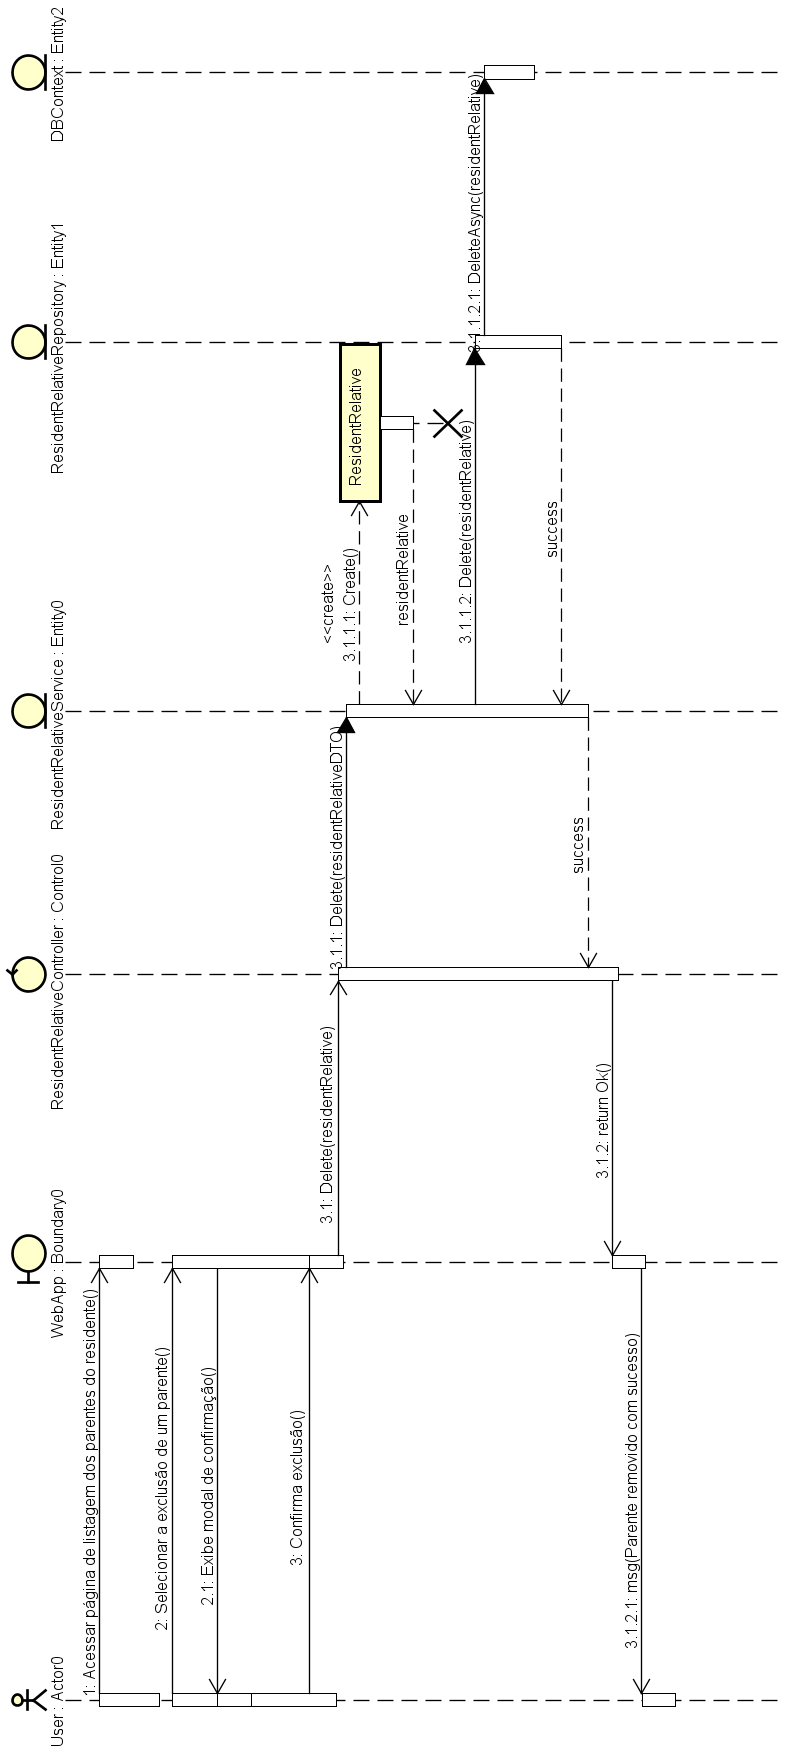
\includegraphics[width=0.45\textwidth]{figs/ResidentRelative_Remover.png}
	\label{fig:seq_remover_residentrelative}
	\fonte{Elaborada pelos autores.}
\end{figure}

Em conjunto, os diagramas analisados permitem uma visão clara do ciclo de vida
completo das operações sobre parentes de residentes, evidenciando o grau de
acoplamento entre as camadas, o fluxo de dados e a ordem das mensagens. Essa
perspectiva dinâmica complementa a visão estrutural oferecida pelos diagramas de
classes, garantindo uma documentação completa, alinhada aos princípios de
engenharia de software estabelecidos pela literatura.

\section{Diagrama de Atividade}

O diagrama de atividade, embora tenha sido inicialmente tratado como um caso especial do diagrama de máquina de estados, é atualmente reconhecido como um diagrama independente dentro da UML. Segundo \textcite[p.~390]{Guedes2018}, trata-se do diagrama com ``mais ênfase em nível de algoritmo da UML e provavelmente um dos mais detalhistas''.

Esse tipo de diagrama é amplamente utilizado na modelagem de \emph{atividades}, entendidas como métodos, algoritmos ou processos completos. Nesse sentido, \textcite[p.~391]{Guedes2018} esclarece que:

\begin{citacao}
	Uma atividade é composta por um conjunto de ações, ou seja, os passos necessários para que a atividade seja concluída.
\end{citacao}

A Figura~\ref{fig:atividade_login} apresenta o diagrama de atividade referente ao fluxo de autenticação do usuário no sistema, ilustrando de forma clara e sequencial as ações realizadas desde o momento em que o usuário insere suas credenciais até a validação final e redirecionamento.

\begin{figure}[H]
	%\centering
	\caption{Diagrama de atividade para o processo de autenticação do usuário.}
	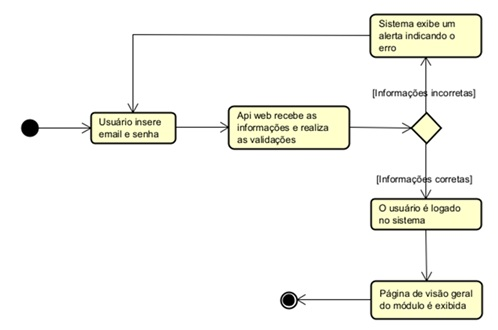
\includegraphics[width=0.95\textwidth]{figs/atividade_login.jpg}
	\label{fig:atividade_login}
	\fonte{Elaborada pelos autores.}
\end{figure}

O diagrama (\ref{fig:atividade_login})inicia-se com o nó inicial (\emph{black node}), indicando o começo do fluxo. Em seguida, o usuário insere seu e-mail e senha, que são enviados à API web responsável por receber e validar essas informações.

Após a etapa de validação, o fluxo se divide em dois caminhos possíveis:

\begin{itemize}
	\item \textbf{Informações incorretas}: o sistema exibe uma mensagem de erro informando que os dados inseridos são inválidos. O fluxo retorna à etapa de inserção das credenciais.
	\item \textbf{Informações corretas}: o usuário é autenticado com sucesso e direcionado à página de visão geral do módulo principal do sistema.
\end{itemize}

Por fim, o diagrama é encerrado pelo nó final, representando o término do processo de autenticação. Esse tipo de modelagem é essencial para evidenciar a lógica de controle do sistema, além de facilitar a comunicação entre desenvolvedores, analistas e demais stakeholders envolvidos no projeto.








\chapter{Definição da Interface com o Usuário}

O design de UX vai muito além da estética: trata-se de compreender contextos,
tarefas e objetivos dos usuários e conectá-los a metas do negócio para produzir
experiências úteis, utilizáveis e desejáveis. Isso envolve investigar o problema,
definir requisitos baseados em evidências, estruturar informação e fluxos,
prototipar soluções, validar com pessoas reais e iterar continuamente com foco em
resultado—acessibilidade, eficiência, satisfação e impacto no negócio.

\textcite{Unger2012} destacam que o(a) designer de UX atua como elo entre áreas
multidisciplinares (produto, engenharia, conteúdo, dados e partes interessadas),
orquestrando do descobrimento à avaliação: pesquisa com usuários, modelagem de
personas e jornadas, construção de \emph{wireframes}/protótipos, testes de
usabilidade e comunicação de decisões. O foco permanece na experiência do usuário,
mas sempre alinhada a objetivos claros e mensuráveis do produto.


\section{Descrição de Cenário}

A descrição de cenário é uma técnica fundamental no processo de design de interação, utilizada para representar situações reais de uso de um sistema ou produto digital. De acordo com \textcite{Rogers2013}, os cenários contribuem para a compreensão do contexto de uso, dos objetivos dos usuários e dos desafios que podem surgir durante a interação. Essas descrições assumem a forma de narrativas simples e acessíveis, que ilustram como um usuário específico realiza tarefas em determinado ambiente. Essa abordagem permite aos designers anteciparem as necessidades e comportamentos, contribuindo para que o produto final esteja alinhado às expectativas e características do público-alvo.

Para ilustrar o comportamento do usuário, foram desenvolvidos dois cenários. Esses cenários descrevem os objetivos dos usuários e as possíveis formas de interação com o sistema, funcionando como narrativas que representam situações reais de uso. Por meio dessas descrições, é possível antecipar como os usuários poderão se relacionar com a interface, contribuindo para um projeto mais alinhado às suas necessidades e expectativas.

Para descrever o processo de cadastro de uma nova religião, foi elaborado o primeiro cenário (Quadro~\ref{quadro:religiao}), que simula como o funcionário pode interagir com o sistema, apresentando uma descrição das etapas envolvidas na inserção das informações de religião.


\begin{quadro}[H]
	\caption[Cenário — Registro de Religião]{Cenário — Registro de Religião por um Funcionário do Lar dos Velhinhos}
	\label{quadro:religiao}
	\begin{tabularx}{\textwidth}{@{}X@{}}
		\toprule
		No contexto de um lar de idosos, uma funcionária administrativa acessa o sistema institucional para cadastrar uma nova religião de um idoso recém-chegado. A funcionária, autenticada no sistema, acessa a página de religiões e clica em ``Nova Religião''. Em seguida, preenche os dados da nova religião, como o nome, e ao concluir o processo clica em ``Salvar''. Essa ação garante que a crença do idoso esteja registrada no sistema, permitindo que suas práticas espirituais sejam respeitadas e consideradas na rotina da instituição.\\
		\bottomrule
	\end{tabularx}
	\fonte{Elaborado pelos autores.}
\end{quadro}

O cenário de consulta médica (Quadro~\ref{quadro:alergia}) apresenta a situação em que um médico utiliza o sistema durante uma consulta clínica com um residente, descrevendo como o sistema permite o acesso ao prontuário digital do paciente, incluindo informações sobre alergias previamente registradas. Com base nesses dados, o médico ajusta a prescrição de medicamentos, assegurando um cuidado seguro, personalizado e compatível com as condições de saúde do residente.

\begin{quadro}[H]
	\caption[Cenário — Registro e Consulta de Alergias]
	{Cenário — Registro e Consulta de Alergias por Médico em Exame}
	\label{quadro:alergia}
	\begin{tabularx}{\textwidth}{@{}X@{}}
		\toprule
	Durante um exame clínico de um residente, o médico, autenticado no sistema, procura o residente pelo nome e acessa o prontuário digital para consultar as alergias previamente registradas. Ao identificar que o residente possui alergia a frutos do mar, o profissional registra cuidadosamente essa informação, preenchendo os campos: tipo da alergia, descrição, data de detecção e, se aplicável, data de liberação, garantindo que toda a instituição esteja ciente da restrição. Em seguida, com base nesses dados, ajusta a prescrição de medicamentos, assegurando um cuidado seguro, individualizado e compatível com as condições de saúde do paciente.\\
		\bottomrule
	\end{tabularx}
	\fonte{Elaborado pelos autores.}
\end{quadro}


\section{Descrição de Personas}

No desenvolvimento centrado no usuário, \textit{personas} funcionam como arquétipos
que sintetizam padrões de comportamento, objetivos, dores e expectativas do público-alvo.
Elas tornam explícito “quem usa o sistema, por quê e em quais condições”, orientando
priorização de requisitos, decisões de navegação e o vocabulário da interface
\parencite{Unger2012}. Conforme a boa prática, não são perfis fictícios arbitrários,
mas representações baseadas em evidências (observação, entrevistas e análise de
processos), e devem ser revisadas à medida que novas descobertas surgirem
\parencite{Unger2012}.

No contexto de um lar de idosos, mapeamos os principais atores que interagem com o
sistema institucional e consolidamos duas \textit{personas} operacionais. O processo
incluiu: (i) levantamento dos fluxos de trabalho e pontos de contato; (ii) coleta de
dados sobre tarefas frequentes, frustrações e critérios de sucesso; (iii) síntese em
arquétipos com objetivos claros; e (iv) validação com as áreas envolvidas. Para cada
\textit{persona} registramos dados demográficos sintéticos, metas, responsabilidades,
tarefas prioritárias e implicações de design (por exemplo, necessidades de acesso
rápido, alertas, permissões e rastreabilidade), de modo a alinhar protótipos e
funcionalidades às demandas reais \parencite{Unger2012}.

\begin{figure}[H]
	%\centering
	\caption{Persona 1 — Enfermeira-chefe (Carla Regina de Souza)}
	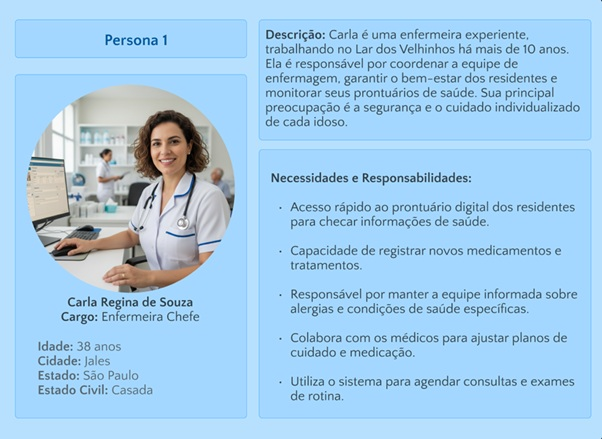
\includegraphics[width=.9\linewidth]{figs/persona01.jpg}
	\label{fig:persona1}
	\fonte{Elaborada pelos autores.}
\end{figure}

A \autoref{fig:persona1} representa “Carla Regina de Souza”, enfermeira-chefe com
experiência na coordenação da equipe e no acompanhamento clínico dos residentes. Suas
necessidades traduzem requisitos concretos do sistema: acesso ágil ao prontuário
digital, registro rápido e seguro de medicamentos e tratamentos, visibilidade de
alergias e condições críticas, agenda de consultas e comunicação com a equipe
multiprofissional. Implicações de design incluem atalhos para tarefas recorrentes,
alertas não intrusivos (por exemplo, alergias), histórico auditável e formulários
otimizados para reduzir retrabalho durante o plantão \parencite{Unger2012}.

\begin{figure}[H]
	%\centering
	\caption{Persona 2 — Recepcionista (Fernando Costa)}
	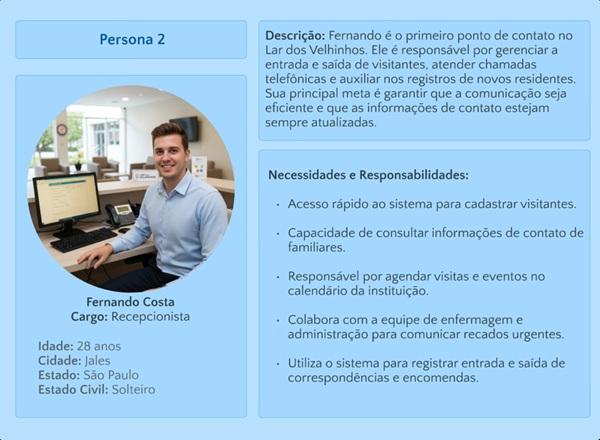
\includegraphics[width=.9\linewidth]{figs/persona02.jpg}
	\label{fig:persona2}
	\fonte{Elaborada pelos autores.}
\end{figure}

A \autoref{fig:persona2} apresenta “Fernando Costa”, recepcionista responsável pela
entrada de visitantes, comunicação com familiares e organização de agendas. Suas
tarefas demandam cadastro e consulta ágeis, calendário institucional claro, registros
de entrada/saída e mecanismos de comunicação confiáveis. Daí decorrem requisitos como
busca por nome/CPF, formulários enxutos, confirmação de identidade e logs de eventos,
além de mensagens de feedback que evitem ambiguidades no atendimento
\parencite{Unger2012}.

Em conjunto, as \textit{personas} estruturam critérios de aceitação e histórias de
usuário (“como \textit{Carla}/\textit{Fernando}, quero \dots para \dots”) e servem de
referência para avaliar protótipos e decisões de priorização ao longo de todo o ciclo
do projeto \parencite{Unger2012}.

\section{Esboços de tela (wireframes)}

\textit{Wireframes} são esboços de baixa fidelidade usados nas etapas iniciais de UX para
tomada de decisão sobre \textbf{arquitetura da informação}, \textbf{hierarquia de
	conteúdo} e \textbf{fluxos de navegação} antes de investir em layout final e código.
Ao abstrair cores, tipografia e imagens, eles mantêm o foco no que é essencial:
quais tarefas o usuário precisa executar, em que ordem, com quais componentes
(campos, botões, listas, filtros) e que \textit{feedback} a interface deve oferecer
(estados vazio/erro/sucesso).

Normalmente apresentados em tons de cinza e com \textit{placeholders}, os wireframes
servem como artefato de alinhamento entre equipes de produto, design e tecnologia.
Eles viabilizam discussões rápidas sobre rótulos, prioridades e regras de negócio,
permitem testes exploratórios com usuários e ajudam a estimar esforço técnico
(\textit{ex.:} dependências de dados, validações, paginação, permissões). Também
facilitam a definição de padrões—grade, espaçamentos, tipos de campo, posição de
ações—que mais tarde serão consolidados no \textit{design system}, assegurando
consistência entre telas e pontos de quebra responsivos.

Na \autoref{fig:wireframe-gestao-religiao}, o wireframe da tela de cadastro/gestão
exemplifica esse padrão funcional: trilha de navegação (\textit{breadcrumbs}) para
contexto, busca por termo, ação primária “\,+ Adicionar\,” e uma listagem tabular com
seleção por linha e ações de \textit{editar}/\textit{excluir}. Esse arranjo evidencia
o fluxo típico de manutenção (localizar \(\rightarrow\) incluir/alterar \(\rightarrow\)
confirmar), reduz a carga cognitiva e estabelece um modelo reutilizável para as demais
telas de registro do sistema, promovendo previsibilidade e menor curva de aprendizado.

As Figuras \ref{fig:wireframe-home}\subref{fig:wireframe-home-care} e
\ref{fig:wireframe-home}\subref{fig:wireframe-home-stock} mostram
\textit{wireframes} de baixa fidelidade para as telas iniciais dos módulos
\emph{Care} e \emph{Stock}. Nesses esboços priorizam‐se mensagem, hierarquia e
\emph{call to action} (CTA), sem preocupação com o acabamento visual, a fim de
validar rapidamente a clareza da proposta e o encaminhamento ao login.

No \textbf{(a) Home Care}, o layout em duas colunas destaca, à esquerda, um
\textbf{título de alto impacto}, \textbf{textinho de apoio} e o CTA
\textbf{Fazer Login}; abaixo, uma faixa de \textbf{atalhos} (prescrições,
cuidados e vacinas) antecipa rotas frequentes do módulo. À direita, reserva‐se
área para \emph{hero} ilustrativo. Já o \textbf{(b) Home Stock} mantém a mesma
estrutura de \emph{hero} (título, apoio e CTA), porém \emph{sem} os atalhos
inferiores, simplificando a entrada e reduzindo a carga cognitiva para o
contexto de estoque. Em ambos, espera‐se responsividade, contraste suficiente,
ordem de leitura previsível e texto alternativo adequado para a imagem.

\begin{figure}[H]
	\caption{Wireframes — (a) Tela Inicial para Módulo de Cuidado (Home Care) e (b) Tela Inicial para Módulo de Estoque (Home Stock)}
	\label{fig:wireframe-home}
	
	\begin{subfigure}[t]{.48\linewidth}
		%\centering
		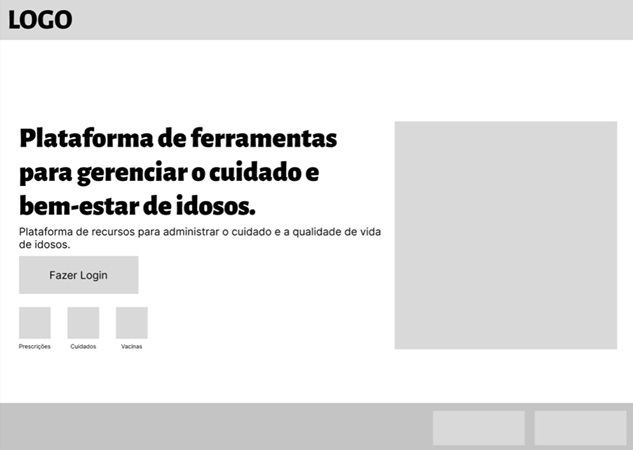
\includegraphics[width=\linewidth]{figs/wireframe_home_care.jpg}
		\caption{Tela Inicial — Home Care}
		\label{fig:wireframe-home-care}
	\end{subfigure}\hfill
	\begin{subfigure}[t]{.48\linewidth}
		%\centering
		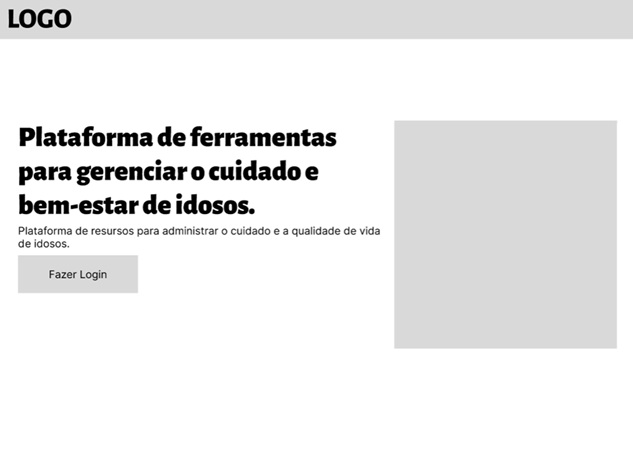
\includegraphics[width=\linewidth]{figs/wireframe_home_stock.jpg}
		\caption{Tela Inicial — Home Stock}
		\label{fig:wireframe-home-stock}
	\end{subfigure}
	
	\fonte{Elaborada pelos autores.}
\end{figure}

As Figuras \ref{fig:wireframe-login}\subref{fig:wireframe-login-care} e
\ref{fig:wireframe-login}\subref{fig:wireframe-login-stock} apresentam
\textit{wireframes} de baixa fidelidade para o fluxo de autenticação dos módulos
\emph{Care} e \emph{Stock}. Por se tratarem de esboços, privilegiam-se hierarquia e
fluxo—não o acabamento visual—para discutir rótulos, ordem dos campos, posicionamento
de ações e mensagens antes da implementação.

Em ambos os casos o formulário \textbf{Login} aparece à esquerda com os campos
\emph{Email} e \emph{Senha} (placeholders/ícones) e a ação primária \textbf{Entrar};
à direita há uma área reservada para imagem institucional. No \textbf{(a) Care},
incluem-se o \emph{checkbox} \emph{Lembrar login} (persistência controlada de
credenciais) e o link \emph{Esqueci minha senha} sob o botão, reforçando conveniência
no acesso domiciliar. No \textbf{(b) Stock}, a omissão do \emph{Lembrar login}
prioriza segurança em ambientes de estoque, mantendo o link de recuperação próximo
ao campo de senha para acesso rápido.

Comportamentos esperados: validação de formato do e-mail, ocultação de caracteres da
senha, estados desabilitado/ativo do botão \textbf{Entrar}, mensagens de erro junto
aos campos e suporte a navegação por teclado e leitores de tela.

\begin{figure}[H]
	\caption{Wireframes — (a) Tela de Login para o Módulo de Cuidado (Care) e (b) Tela de Login para o Módulo de Estoque (Stock)}
	\label{fig:wireframe-login}
	
	\begin{subfigure}[t]{.48\linewidth}
		%\centering
		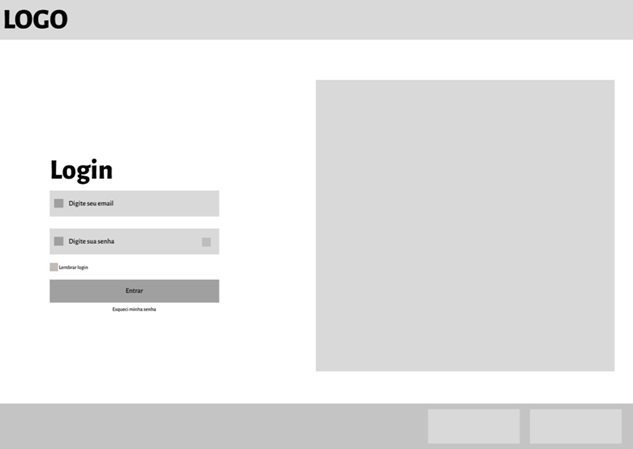
\includegraphics[width=\linewidth]{figs/wireframe_login_care.jpg}
		\caption{Tela de Login — Care}
		\label{fig:wireframe-login-care}
	\end{subfigure}\hfill
	\begin{subfigure}[t]{.48\linewidth}
		%\centering
		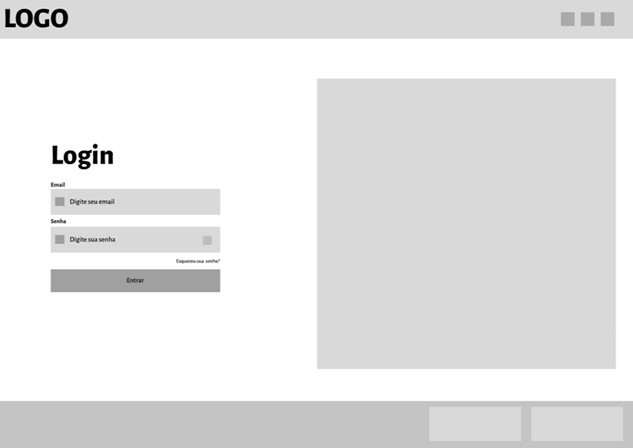
\includegraphics[width=\linewidth]{figs/wireframe_login_stock.jpg}
		\caption{Tela de Login — Stock}
		\label{fig:wireframe-login-stock}
	\end{subfigure}
	
	\fonte{Elaborada pelos autores.}
\end{figure}

As Figuras \ref{fig:wireframe-cadastro}\subref{fig:wireframe-cadastro-instituicao} e
\ref{fig:wireframe-cadastro}\subref{fig:wireframe-gestao-religiao} apresentam
\textit{wireframes} de baixa fidelidade que documentam os padrões de cadastro do
projeto. Esses esboços priorizam fluxo e hierarquia de informação (e não o
acabamento visual), permitindo discutir campos obrigatórios, ações primárias e
navegação antes da implementação.

O \textbf{wireframe (a)} ilustra o \emph{cadastro de produto}: trilha de navegação
(\emph{Visão Geral} $\rightarrow$ \emph{Cadastros} $\rightarrow$ \emph{Produto}
$\rightarrow$ \emph{Cadastro Produto}), campo de busca global e formulário em duas
colunas com metadados essenciais (nome genérico, descrição, tipo, grupo, unidade de
medida), opções operacionais (controle de validade, estoque atual/mínimo) e a ação
primária \textbf{Cadastrar produto}. Já o \textbf{wireframe (b)} representa a
\emph{gestão de religiões}: busca por nome, botão \textbf{+ Adicionar}, e listagem
tabular com seleção por linha e ações de \emph{editar}/\emph{excluir}. Em conjunto,
as telas evidenciam o padrão do sistema para criação e manutenção de registros.

\begin{figure}[H]
	\caption{Wireframes — (a) Tela de Cadastro de Instituição e (b) Tela de Gestão de Religião}
	\label{fig:wireframe-cadastro}
	
	\begin{subfigure}[t]{.48\linewidth}
		%\centering
		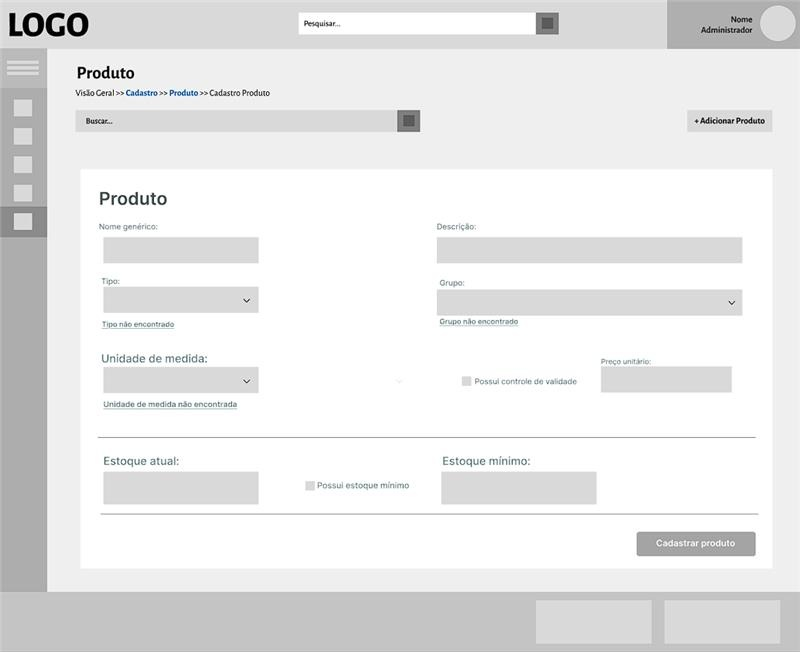
\includegraphics[width=\linewidth]{figs/wireframe_cadastro_produto.jpg}
		\caption{Cadastro de Instituição}
		\label{fig:wireframe-cadastro-instituicao}
	\end{subfigure}\hfill
	\begin{subfigure}[t]{.48\linewidth}
		%\centering
		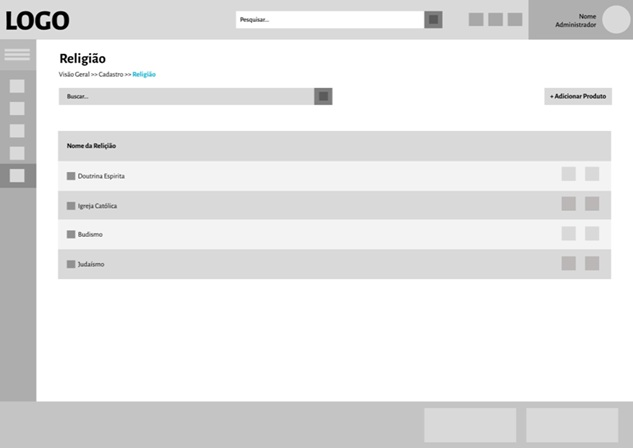
\includegraphics[width=\linewidth]{figs/wireframe_gestao_religiao.jpg}
		\caption{Gestão de Religião}
		\label{fig:wireframe-gestao-religiao}
	\end{subfigure}
	
	\fonte{Elaborada pelos autores.}
\end{figure}


\section{Protótipos de tela}

Protótipos de tela são representações visuais (estáticas ou interativas) que simulam a
interface e o comportamento de um sistema, permitindo explorar ideias, validar hipóteses
de uso e antecipar ajustes antes do investimento em desenvolvimento. \textcite{Rosa2025}
classifica-os quanto à fidelidade em baixa, média e alta: os de \emph{baixa} apoiam a
ideação rápida e o alinhamento conceitual; os de \emph{média} permitem refinar fluxos,
rótulos e hierarquia de informação; e os de \emph{alta} aproximam-se do produto final,
servindo à validação de microinterações, estados e conteúdo. Já \textcite{Garrett2011}
enquadra a prototipagem nos planos de \emph{estrutura} e \emph{superfície} da experiência
do usuário, não apenas como representação estética, mas como instrumento estratégico para
avaliar a disposição de elementos, os fluxos de navegação e a usabilidade de ponta a ponta.

Como prática, a prototipagem deve ser iterativa: hipóteses são materializadas em telas,
testadas com usuários e partes interessadas, e os aprendizados retornam ao modelo em ciclos
sucessivos de melhoria. Esse processo reduz riscos, acelera decisões de design, favorece o
alinhamento entre equipes e produz artefatos que comunicam requisitos de forma mais clara
do que especificações exclusivamente textuais \parencite{Garrett2011,Rosa2025}.

No projeto \emph{SeniorCareManager}, utilizou-se o Figma para produzir protótipos de
\emph{alta fidelidade} com interações navegáveis, estados de componentes e variações de
telas responsivas. O uso de bibliotecas de componentes e estilos consolidou padrões visuais
e de interação, facilitando testes de usabilidade e o \emph{handoff} para desenvolvimento,
com insumos precisos sobre hierarquia, fluxos críticos e microcomportamentos
\parencite{Rosa2025,Garrett2011}.


A \autoref{fig:proto-abertura-care} apresenta a tela de abertura (\emph{hero}) do
\emph{SeniorCareManager}. O layout em duas colunas prioriza a comunicação da proposta
de valor e a ação principal: à esquerda, um \textbf{título de alto destaque} e um
\textbf{textinho de apoio} introduzem o objetivo de gerenciar cuidado e bem-estar de
idosos, seguido do botão primário \textbf{Fazer login}, que conduz ao fluxo de
autenticação. Abaixo, uma faixa de \textbf{atalhos com ícones} oferece acesso rápido
às áreas mais usadas do sistema (por exemplo, prontuários, cuidados, ocorrências e
vacinas), reforçando a orientação a tarefas. À direita, uma \textbf{imagem
	contextual} transmite a ideia de acolhimento e cuidado.

A composição privilegia hierarquia tipográfica, espaçamento generoso e uma única
chamada para ação, reduzindo a carga cognitiva na primeira interação. A imagem
ilustrativa pode ser adaptada ao tema (alto contraste ou não) e, quando marcada como
decorativa, utiliza texto alternativo vazio para não interferir na navegação por
leitores de tela. O resultado é uma porta de entrada simples, responsiva e
acessível, que direciona o usuário ao próximo passo do uso do sistema.


\begin{figure}[H]
	%\centering
	\caption{SeniorCareManager — Tela de Abertura}
	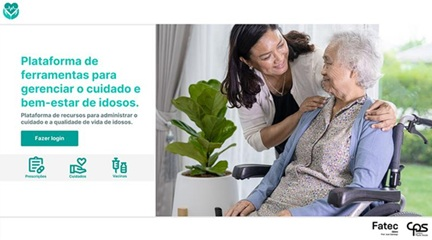
\includegraphics[width=.9\linewidth]{figs/prototipo_abertura_care.jpg}
	\label{fig:proto-abertura-care}
	\fonte{Elaborado pelos autores.}
\end{figure}

A \autoref{fig:proto-abertura-stock} apresenta a tela de abertura (\emph{landing/hero})
do \emph{SeniorStockManager}. O layout em duas colunas prioriza a mensagem central e a
ação principal: à esquerda, um \textbf{título de alto contraste} comunica a proposta de
valor da plataforma, seguido de um \textbf{textinho de apoio} e do \textbf{botão primário
	“Fazer Login”}, que conduz ao fluxo de autenticação. À direita, uma \textbf{ilustração
	temática} relacionada a estoque e conferência reforça o contexto do módulo.

A composição privilegia hierarquia tipográfica, espaçamento generoso e foco em uma única
chamada para ação, reduzindo a carga cognitiva e facilitando a decisão do usuário. A
ilustração é carregada dinamicamente e se adapta ao tema selecionado, preservando legibilidade
e contraste; quando marcada como decorativa, utiliza texto alternativo vazio para não
interferir na navegação por leitores de tela. O resultado é uma tela de boas-vindas simples,
orientada a objetivos e alinhada a boas práticas de usabilidade e acessibilidade.

\begin{figure}[H]
	%\centering
	\caption{SeniorStockManager — Tela de Abertura}
	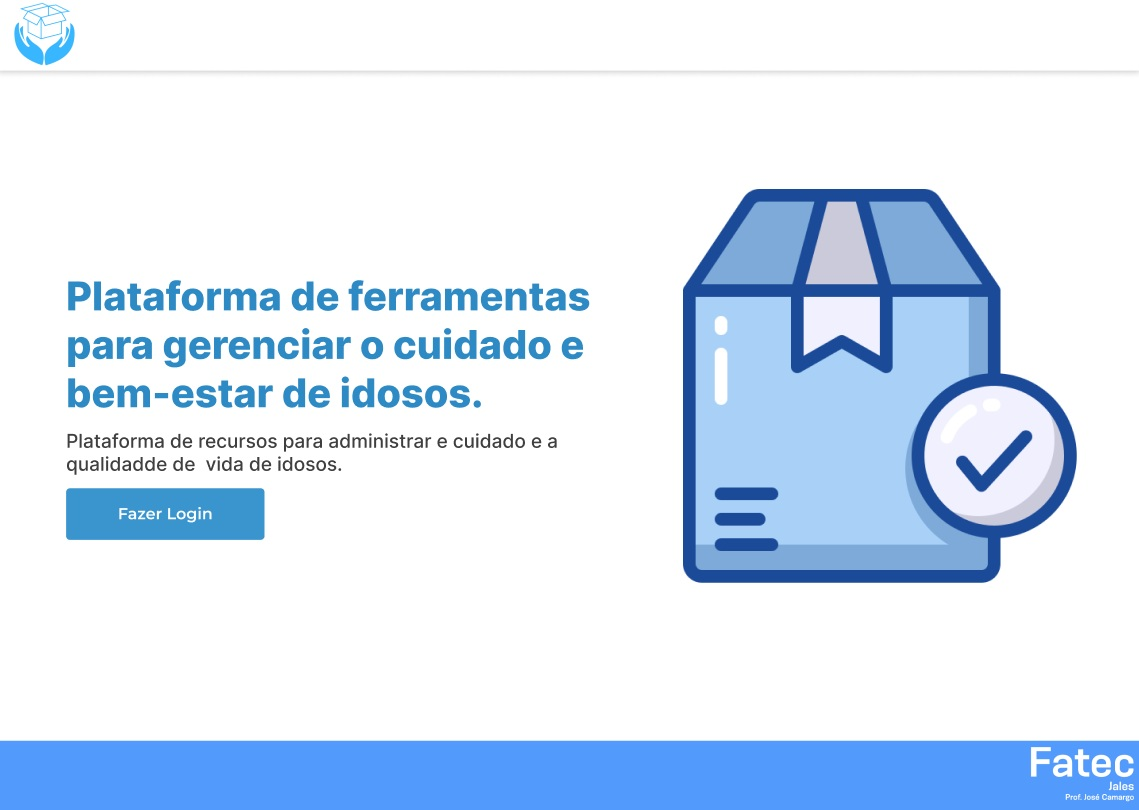
\includegraphics[width=.9\linewidth]{figs/prototipo_abertura_stock.jpg}
	\label{fig:proto-abertura-stock}
	\fonte{Elaborado pelos autores.}
\end{figure}

A \autoref{fig:proto-login-care} apresenta a tela de autenticação do
\emph{SeniorCareManager}. O layout em duas colunas destaca, à esquerda, o formulário
\textbf{Login} com campos \emph{Email} e \emph{Senha} (com \emph{placeholders} e ícones),
a opção \emph{Lembrar login}, o botão primário \textbf{Entrar} e o link
\emph{Esqueci minha senha}. À direita, uma imagem temática reforça a proposta de
cuidado e acolhimento do módulo. A organização privilegia hierarquia visual e foco
na tarefa: rotulagem acima dos campos, áreas de ação bem delimitadas e espaçamento
regular. Comportamentos esperados incluem validação do formato de e-mail, ocultação
dos caracteres de senha, mensagens de erro junto aos campos, persistência controlada
das credenciais quando o \emph{checkbox} é ativado, além de suporte a navegação por
teclado e leitura por tecnologias assistivas.

\begin{figure}[H]
	%\centering
	\caption{SeniorCareManager — Tela de Login}
	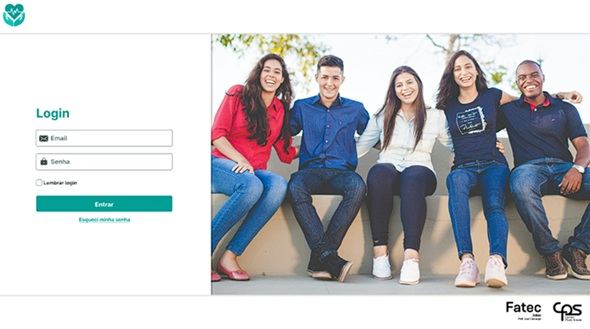
\includegraphics[width=.9\linewidth]{figs/prototipo_login_care.jpg}
	\label{fig:proto-login-care}
	\fonte{Elaborado pelos autores.}
\end{figure}

A \autoref{fig:proto-login-stock} apresenta a tela de autenticação do
\emph{SeniorStockManager}. À esquerda, o formulário \textbf{Login} dispõe dos campos
\emph{Email} e \emph{Senha} com \emph{placeholders} (“Digite seu email”, “Digite sua
senha”), ícones de apoio nos \emph{inputs}, link \emph{Esqueceu sua senha?} e o botão
primário \textbf{Entrar}. À direita, uma ilustração temática de caixas/estoque reforça o
contexto do módulo. O layout em duas colunas é responsivo e privilegia hierarquia
visual (título destacado, rótulos acima dos campos e áreas de ação bem delimitadas),
promovendo leitura rápida e clara. O fluxo principal consiste em informar as credenciais
e acionar \textbf{Entrar}; regras usuais incluem validação de formato para e-mail,
ocultação de caracteres no campo de senha e exibição de mensagens de erro junto aos
campos quando necessário, além do atalho para recuperação de credenciais via link.

\begin{figure}[H]
	%\centering
	\caption{SeniorStockManager — Tela de Login}
	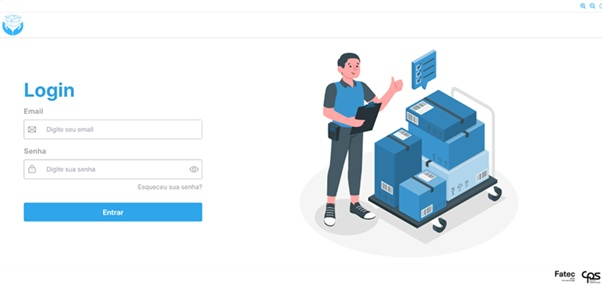
\includegraphics[width=.9\linewidth]{figs/prototipo_login_stock.jpg}
	\label{fig:proto-login-stock}
	\fonte{Elaborado pelos autores.}
\end{figure}

A \autoref{fig:proto-cadastro-religiao} apresenta a tela de \emph{gestão de religiões}
do \emph{SeniorCareManager}. A interface organiza o fluxo de manutenção em três áreas
claras: (i) \textbf{contexto e navegação}, com trilha “Visão Geral \(\rightarrow\) Cadastros
\(\rightarrow\) Religião” e campo de busca por nome; (ii) \textbf{ação primária} “+ Adicionar
religião” para inclusão de novos registros; e (iii) \textbf{listagem tabular} “Nome da
religião”, com seleção por linha e ações contextuais de \emph{editar} (ícone de lápis) e
\emph{excluir} (ícone de lixeira). Esse arranjo permite localizar rapidamente um registro,
criar novos itens e manter o cadastro atualizado por meio de operações pontuais sobre cada
entrada, preservando a consistência das informações institucionais.

\begin{figure}[H]
	%\centering
	\caption{SeniorCareManager — Gestão de Religiões (listagem, busca e manutenção)}
	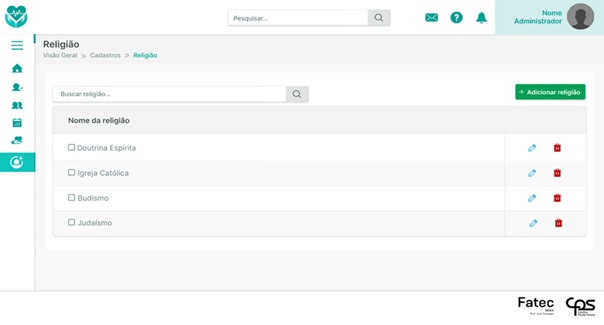
\includegraphics[width=.9\linewidth]{figs/prototipo_cadastro_religiao.jpg}
	\label{fig:proto-cadastro-religiao}
	\fonte{Elaborado pelos autores.}
\end{figure}

A \autoref{fig:proto-cadastro-produto} apresenta a tela de manutenção de produtos do
\emph{SeniorStockManager}. A área superior fornece \textbf{contexto e navegação}, com a
trilha “Visão Geral $\rightarrow$ Cadastros $\rightarrow$ Produto $\rightarrow$ Cadastro Produto”
e um campo de \emph{busca} global. O formulário \textbf{Produto} é organizado em duas
colunas e reúne os principais metadados do item: \emph{Nome genérico} e \emph{Descrição};
listas suspensas para \emph{Tipo} e \emph{Grupo}, acompanhadas de atalhos “Tipo não
encontrado” e “Grupo não encontrado” para inclusão rápida de classificações ausentes;
\emph{Unidade de medida} (com link “Unidade de medida não encontrada”); opção
\emph{Possui controle de validade} (habilita o acompanhamento por data de vencimento);
\emph{Preço unitário}; \emph{Estoque atual} e \emph{Estoque mínimo}, com o seletor
\emph{Possui estoque mínimo} para ativar a regra de reposição. O fluxo principal consiste
em informar os atributos do produto, selecionar suas classificações e unidade, definir
regras de validade e de estoque e, por fim, confirmar a inclusão por meio do botão
\textbf{Cadastrar produto}. Essa organização favorece a consistência cadastral e a
manutenção contínua do catálogo, reduzindo retrabalho e erros operacionais.

\begin{figure}[H]
	%\centering
	\caption{SeniorStockManager — Tela de Manutenção de Produtos}
	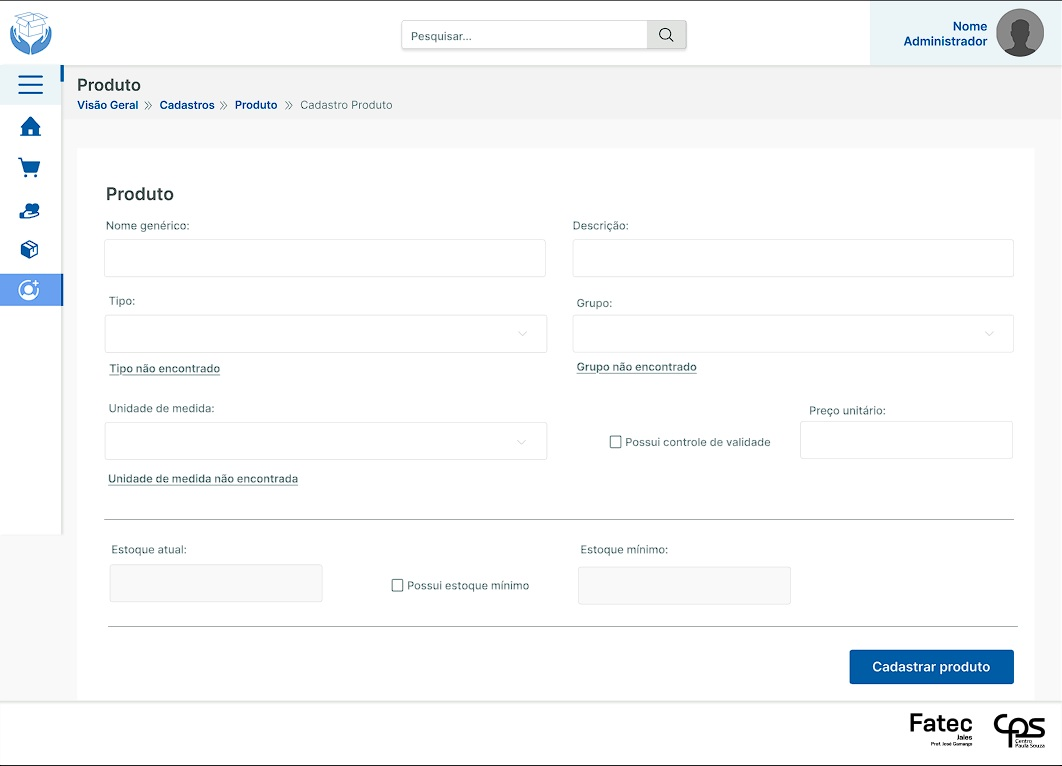
\includegraphics[width=.9\linewidth]{figs/prototipo_cadastro_produto.jpg}
	\label{fig:proto-cadastro-produto}
	\fonte{Elaborado pelos autores.}
\end{figure}

\section{Acessibilidade e Inclusão de Pessoas com Deficiência}

A inclusão de pessoas com deficiência (PCD) constitui um tema de grande relevância para a sociedade contemporânea. De acordo com a \textcite{OMS2011}, aproximadamente 1 bilhão de pessoas em todo o mundo vive com algum tipo de deficiência, o que equivale a cerca de uma em cada sete pessoas. A Convenção Internacional sobre os Direitos das Pessoas com Deficiência, assinada em Nova Iorque em 2007 e ratificada no Brasil pelo Decreto nº 6.949, de 25 de agosto de 2009 \parencite{Brasil2009}, define como pessoas com deficiência aquelas que apresentam impedimentos de longa duração, sejam eles de ordem física, mental, intelectual ou sensorial, os quais, em interação com barreiras diversas, podem restringir sua plena participação na sociedade.

Para combater o preconceito e assegurar a igualdade de oportunidades, torna-se indispensável a adoção de medidas que envolvem a adaptação de espaços físicos, a adequação da linguagem, o uso de tecnologias inclusivas e a promoção da inserção no mercado de trabalho. Tais ações são fundamentais para garantir que as PCD possam viver de forma independente e participar plenamente da vida social.

A promoção da acessibilidade implica assegurar condições de acesso igualitário ao meio físico, ao transporte, à informação e à comunicação, incluindo os sistemas e tecnologias digitais, bem como a outros serviços e instalações disponíveis ao público. Apesar dos direitos assegurados por documentos internacionais, como a Declaração Universal dos Direitos Humanos, e por recomendações da própria OMS, ainda persistem barreiras significativas que comprometem a efetivação desses direitos. O engajamento coletivo da sociedade é, portanto, essencial para a eliminação de obstáculos e formas de discriminação, configurando-se como um dever social e ético em prol da construção de um mundo mais justo e inclusivo.

No âmbito digital, a acessibilidade refere-se à eliminação de barreiras na web, garantindo que páginas e portais sejam projetados de forma que todas as pessoas possam perceber, compreender, navegar e interagir de maneira eficaz com os conteúdos e serviços oferecidos. O objetivo é democratizar o acesso e assegurar que todos, independentemente de suas condições físico-motoras, perceptivas, culturais ou sociais, consigam usufruir plenamente dos recursos digitais.

As barreiras digitais representam um desafio significativo. Segundo dados do \textcite{IBGE2010}, cerca de 45 milhões de brasileiros possuem algum tipo de deficiência, representando 23,9\% da população nacional. Esse cenário evidencia a urgência de um ambiente digital inclusivo. A implementação de práticas de acessibilidade digital não apenas democratiza o acesso, mas também favorece a inclusão social, possibilitando que pessoas com deficiência utilizem a internet para estudar, trabalhar, realizar compras e compartilhar experiências, sem a necessidade de deslocamento físico.

Além disso, um site acessível tende a apresentar maior compatibilidade com diferentes dispositivos e aplicativos, além de ser melhor indexado por mecanismos de busca. Assim, os benefícios da acessibilidade digital estendem-se não apenas às pessoas com deficiência, mas também a idosos e a usuários com menor familiaridade com ferramentas digitais ou que dependem de dispositivos móveis. Dessa forma, a acessibilidade digital configura-se como um princípio de justiça social, cuja finalidade é garantir que todos possam participar plenamente da sociedade moderna.

\subsection{Práticas de Acessibilidade Implementadas}

Após um estudo detalhado das práticas de acessibilidade recomendadas para sistemas web, foram aplicadas diretrizes que asseguram uma experiência inclusiva para todos os usuários. Essas práticas estão fundamentadas nas recomendações internacionais das \textit{Web Content Accessibility Guidelines} (WCAG 2.1) \parencite{WCAG2018}, bem como nas normativas brasileiras, representadas pelo Decreto nº 5.296/2004 \parencite{Brasil2004} e pela Lei Brasileira de Inclusão da Pessoa com Deficiência (Lei nº 13.146/2015) \parencite{Brasil2015}. Tais medidas visam aprimorar a navegação, a usabilidade e a compreensão do conteúdo, garantindo equidade de acesso a pessoas com diferentes tipos de deficiência.

Entre as práticas adotadas, destaca-se a inclusão de textos alternativos em todas as imagens do sistema, permitindo que leitores de tela transmitam o conteúdo visual a usuários com deficiência visual. Esse recurso assegura que os elementos gráficos tenham significado mesmo quando não podem ser visualizados diretamente.

Outro recurso essencial foi a implementação de teclas de atalho que possibilitam a navegação sem a utilização do mouse, atendendo especialmente às necessidades de pessoas com limitações motoras. A Tabela~\ref{tab:atalhos} apresenta as principais combinações de teclas definidas no sistema, bem como suas funções.

Esses atalhos desempenham papel fundamental na acessibilidade do sistema, pois possibilitam a reversão rápida de ações incorretas, o acesso imediato a funções críticas como salvar ou imprimir documentos, a alternância entre diferentes seções e a navegação fluida entre elementos interativos. Além disso, recursos como o fechamento ágil de janelas modais e o acesso ao topo da página contribuem para reduzir barreiras e garantir maior autonomia ao usuário.

A acessibilidade também foi fortalecida por meio da organização semântica do conteúdo, estruturada de forma lógica para facilitar a interpretação por leitores de tela. Esse recurso permite que títulos, subtítulos e parágrafos sejam identificados corretamente, garantindo que a hierarquia informacional seja preservada. 

\begin{table}[H]
	%\centering
	\caption{Teclas de Atalho Definidas no Sistema}
	\label{tab:atalhos}
	\renewcommand{\arraystretch}{1.3}
	\setlength{\tabcolsep}{8pt}
	\begin{tabular}{ll}
		\toprule
		\textbf{Tecla} & \textbf{Função} \\
		\midrule
		Alt + Z & Desfazer a última ação \\
		Alt + Y & Refazer a ação desfeita \\
		Alt + T & Selecionar todo o conteúdo \\
		Alt + G & Abrir a caixa de busca de texto \\
		Alt + D & Salvar o documento ou projeto atual \\
		Alt + W & Alternar entre janelas abertas \\
		Ctrl + $\rightarrow$ & Navegar entre elementos interativos \\
		Ctrl + $\leftarrow$ & Retornar ao elemento anterior \\
		Alt + X & Fechar janelas modais ou menus \\
		Alt + P & Imprimir o documento atual \\
		Alt + N & Abrir nova janela ou documento \\
		F2 & Abrir a ajuda do sistema \\
		Alt + C & Fechar a janela ativa \\
		Alt + U & Ir ao topo da página \\
		\bottomrule
	\end{tabular}
	\legend{Elaborado pelo autor.}
\end{table}

A implementação de práticas de acessibilidade no sistema tem como objetivo assegurar que pessoas com diferentes tipos de deficiência possam utilizá-lo de forma plena e inclusiva. As diretrizes adotadas estão em conformidade com as recomendações das \textit{Web Content Accessibility Guidelines} (WCAG 2.1) \parencite{WCAG2018}, com o Decreto nº 5.296/2004 \parencite{Brasil2004} e com a Lei Brasileira de Inclusão da Pessoa com Deficiência (Lei nº 13.146/2015) \parencite{Brasil2015}. A seguir, são descritos os principais recursos desenvolvidos.

Outro aspecto fundamental implementado no sistema foi o contraste adequado entre texto e fundo, assegurando maior legibilidade, sobretudo para pessoas com baixa visão ou daltonismo. Para isso, foi disponibilizada uma opção de \textbf{alto contraste}, ativada por meio de um ícone localizado no canto superior direito de todas as telas, que aplica uma paleta neutra composta por preto, branco e cinza. Essa solução amplia a clareza e a simplicidade visual, reduz a sobrecarga cognitiva dos usuários e garante consistência da experiência tanto na versão para \textit{desktop} quanto para dispositivos móveis.

A Figura  \ref{fig:alto-contraste} apresenta a interface de login em sua versão para \textit{desktop}, permitindo a comparação entre o modo com alto contraste ativado (Figura \ref{fig:alto-contraste}\subref{fig:login-contraste}) e a versão sem o recurso (Figura \ref{fig:alto-contraste}\subref{fig:login-sem-contraste}). Observa-se que o alto contraste proporciona maior destaque aos elementos da interface, favorecendo a leitura e interação dos usuários.  

\begin{figure}[H]
	%\centering
	\caption{Alto Contraste — (a) Tela de login com alto contraste ativado e (b) Tela de login sem alto contraste}
	\label{fig:alto-contraste}
	
	\begin{subfigure}[t]{\linewidth}
		%\centering
		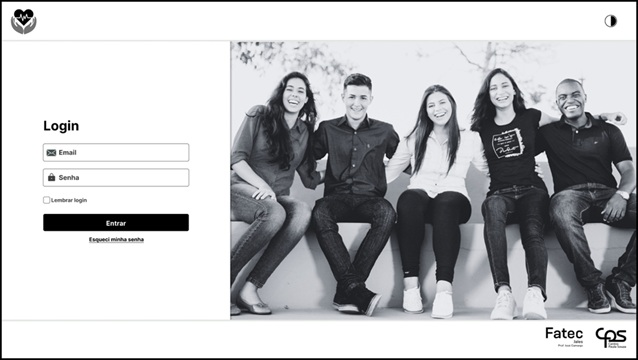
\includegraphics[width=0.7\textwidth]{figs/login_alto_contraste.jpg}
		\caption{Tela de login com o recurso de alto contraste ativado.}
		\label{fig:login-contraste}
	\end{subfigure}
	
	\vspace{0.5cm} % espaço vertical entre as imagens
	
	\begin{subfigure}[t]{\linewidth}
		%\centering
		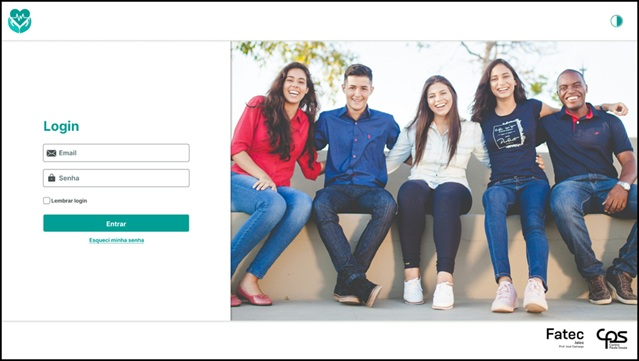
\includegraphics[width=0.7\textwidth]{figs/login_sem_alto_contraste.jpg}
		\caption{Tela de login com o recurso de alto contraste desativado.}
		\label{fig:login-sem-contraste}
	\end{subfigure}
	
	\fonte{Elaborada pelos autores.}
\end{figure}


De forma complementar, a figura \ref{fig:alto_contraste_mobile} ilustra a aplicação do mesmo recurso em dispositivos móveis, destacando a consistência da solução. Na Figura \ref{fig:alto_contraste_mobile}\subref{fig:login-contraste_mobile} está representada a tela de login com alto contraste ativado, enquanto a Figura \ref{fig:alto_contraste_mobile}\subref{fig:login-sem-contraste_mobile} mostra a versão sem contraste. Essa adaptação garante que a acessibilidade seja mantida em diferentes plataformas, assegurando a inclusão digital de forma equitativa.

\begin{figure}[H]
	\caption{Alto Contraste — Dispositivos Móveis — (a) Tela de login com alto contraste ativado e (b) Tela de login sem alto contraste}
	\label{fig:alto_contraste_mobile}
	
	\begin{subfigure}[t]{.48\linewidth}
		%\centering
		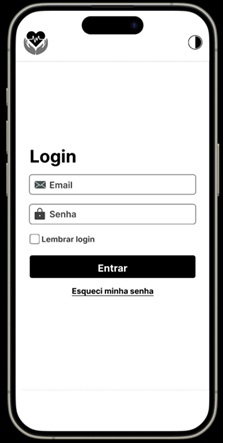
\includegraphics[width=0.75\textwidth]{figs/login_alto_contraste_mobile.jpg}
		\caption{Tela de login com o recurso de alto contraste ativado.}
		\label{fig:login-contraste_mobile}
	\end{subfigure}\hfill
	\begin{subfigure}[t]{.48\linewidth}
		%\centering
		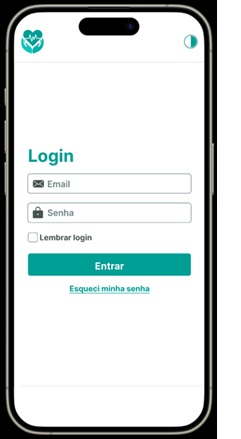
\includegraphics[width=0.75\textwidth]{figs/login_sem_alto_contraste_mobile.jpg}
		\caption{Tela de login com o recurso de alto contraste desativado.}
		\label{fig:login-sem-contraste_mobile}
	\end{subfigure}
	
	\fonte{Elaborada pelos autores.}
\end{figure}

Outro recurso implementado foi o \textbf{texto redimensionável}, que possibilita ao usuário ajustar dinamicamente o tamanho das fontes sem comprometer a disposição ou a legibilidade do conteúdo exibido. Essa funcionalidade é especialmente relevante para pessoas com dificuldades visuais, pois oferece maior conforto na leitura e reduz o esforço cognitivo durante a navegação. Além disso, o recurso beneficia a utilização em diferentes dispositivos, como tablets e smartphones, assegurando que o conteúdo mantenha sua clareza e organização independentemente do tamanho da tela.  

A Figura \ref{fig:fonte-redimensionavel} ilustra a aplicação prática desse recurso, apresentando a tela principal do sistema (Figura \ref{fig:fonte-redimensionavel}\subref{fig:tela-principal-redim}) e o menu lateral (Figura \ref{fig:fonte-redimensionavel}\subref{fig:tela-principal-menu-redim}) com o texto redimensionado. Observa-se que, mesmo com o aumento do tamanho da fonte, a interface preserva sua estrutura e mantém a usabilidade, garantindo uma experiência inclusiva e acessível para todos os usuários.
 

\begin{figure}[H]
	%\centering
	\caption{Fonte Redimensionada - (a) Tela principal (b) Menu Lateral com fonte redimensinada.}
	\label{fig:fonte-redimensionavel}
	
	\begin{subfigure}[t]{\linewidth}
	%	\centering
		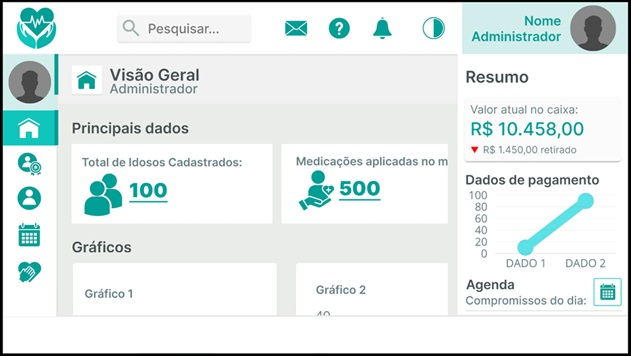
\includegraphics[width=0.7\textwidth]{figs/tela_principal_redim.jpg}
		\caption{Tela principal com a fonte redimensionada.}
		\label{fig:tela-principal-redim}
	\end{subfigure}
	
	\vspace{0.5cm} % espaço vertical entre as imagens
	
	\begin{subfigure}[t]{\linewidth}
	%	\centering
		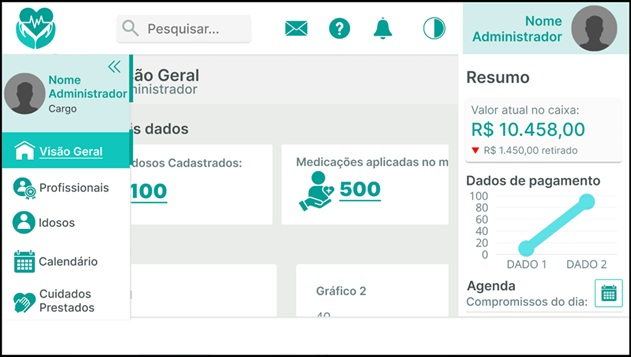
\includegraphics[width=0.7\textwidth]{figs/tela_principal_menu_redim.jpg}
		\caption{Tela principal com o menu lateral com fonte redimensionada.}
		\label{fig:tela-principal-menu-redim}
	\end{subfigure}
	
	\fonte{Elaborada pelos autores.}
\end{figure}

Além das práticas já descritas, outros recursos foram identificados como essenciais para assegurar a acessibilidade em sistemas informatizados. Entre eles, destaca-se a \textbf{compatibilidade com leitores de tela}, que garante que todos os elementos interativos, como botões, menus e campos de formulário, sejam corretamente interpretados e compreendidos por pessoas com deficiência visual. Essa funcionalidade possibilita que tecnologias assistivas transmitam de forma precisa o conteúdo, assegurando maior autonomia ao usuário.  

Outro aspecto relevante é o \textbf{foco visível}, implementado em botões, links e outros elementos interativos, de modo que sejam destacados visualmente quando acessados por meio da navegação via teclado. Essa medida favorece principalmente pessoas com dificuldades motoras ou usuários que não utilizam o mouse, permitindo identificar com clareza o ponto de interação na interface.  

Para promover uma experiência mais inclusiva e menos invasiva, o sistema evita a reprodução automática de mídias, adotando a prática de \textbf{não utilizar autoplay}. Dessa forma, o usuário mantém total controle sobre o início e o término de áudios e vídeos, o que contribui para a concentração, reduz distrações e assegura a compatibilidade com ferramentas de apoio tecnológico.  

A \textbf{facilidade de fechamento} também foi considerada, permitindo que janelas modais e pop-ups sejam encerradas de maneira simples, tanto por cliques visuais quanto pela navegação via teclado. Esse recurso impede que o usuário fique preso em elementos da interface, preservando a fluidez da navegação.  

Outro recurso de destaque é o \textbf{suporte a múltiplas línguas}, com a correta definição da linguagem principal das páginas. Essa prática facilita a atuação de tradutores automáticos e leitores de tela, garantindo interpretação adequada do conteúdo, com leitura e pronúncia precisas.  

Para orientar a navegação dentro do sistema, foi implementado o recurso de \textbf{breadcrumbs} (migalhas de pão), que exibe ao usuário o caminho percorrido até a página atual. Isso favorece o entendimento da hierarquia do site e facilita a localização de conteúdos.  

Além disso, todos os conteúdos multimídia foram planejados de forma acessível. Os \textbf{vídeos possuem legendas} e os conteúdos em áudio são acompanhados de transcrições, assegurando que pessoas com deficiência auditiva também tenham acesso completo às informações apresentadas.  

A \textbf{formatação clara e consistente} do layout foi priorizada, com uso de espaçamento adequado, organização lógica e padronização visual. Essa estrutura beneficia todos os usuários, em especial aqueles com deficiência cognitiva, que necessitam de maior clareza para compreender informações.  

Outro ponto importante é o \textbf{feedback acessível}, em que mensagens de erro e avisos do sistema são apresentados de forma simples, direta e acompanhados de explicações visuais e textuais. Esse recurso garante que o usuário saiba identificar falhas e entenda como corrigi-las de forma eficiente.  

Por fim, assegurou-se o \textbf{desempenho em dispositivos móveis}, mantendo as boas práticas de acessibilidade tanto em celulares quanto em tablets. Isso permite que a experiência inclusiva seja preservada em diferentes plataformas, garantindo a universalidade do acesso às funcionalidades do sistema.

Em síntese, a combinação de alto contraste, texto redimensionável, compatibilidade com leitores de tela, foco visível, suporte a múltiplos idiomas, navegação assistida e conteúdos multimídia acessíveis reflete o compromisso com a inclusão digital, assegurando que todos os usuários possam interagir com o sistema de maneira equitativa e eficaz.


\chapter{Banco de Dados}

Os dados constituem um ativo central em sistemas de informação: deles derivam relatórios, análises e funcionalidades críticas do negócio. Nessa perspectiva, um banco de dados pode ser definido como um conjunto organizado de dados relacionados que representam aspectos do mundo real, armazenados com um propósito específico e de forma a permitir recuperação e atualização consistentes \parencite{Machado2020}.

Dentre os paradigmas de armazenamento, o modelo relacional permanece hegemônico no processamento transacional e analítico de grande parte das aplicações. Nesse modelo, a informação é estruturada em tabelas (relações) formadas por tuplas (linhas) e atributos (colunas), sob um esquema que explicita domínios, chaves e restrições de integridade \parencite{Silberschatz2012}. Em um processo típico de projeto, parte-se de um modelo conceitual (E-R), mapeiam-se entidades e relacionamentos para o modelo lógico relacional e, por fim, define-se o esquema físico com chaves primárias e estrangeiras, índices e restrições. A normalização reduz redundâncias e anomalias de atualização, enquanto a criação criteriosa de índices e \emph{views} apoia desempenho e legibilidade das consultas \parencite{Silberschatz2012}.

No contexto deste projeto, adotou-se o PostgreSQL como SGBD relacional para gerenciar e processar o fluxo de dados de forma eficiente. Trata-se de uma plataforma objeto–relacional de código aberto, apta a implementar chaves, restrições, \emph{triggers}, funções e consultas complexas, alinhando-se às necessidades de integridade e desempenho esperadas em sistemas corporativos \parencite{Silberschatz2012}.

Operações de acesso e atualização são agrupadas em transações, unidades lógicas de trabalho que devem preservar as propriedades \emph{ACID} \parencite{Silberschatz2012}: (i) \textbf{atomicidade}, garantindo que todas as ações de uma transação sejam aplicadas integralmente ou, em caso de falha, nenhuma o seja; (ii) \textbf{consistência}, assegurando que o banco de dados transite apenas entre estados válidos; (iii) \textbf{isolamento}, evitando que execuções concorrentes interfiram entre si e produzam leituras sujas, não repetíveis ou fenômenos de fantasma; e (iv) \textbf{durabilidade}, pela qual os efeitos de uma transação confirmada permanecem mesmo diante de falhas do sistema. Em conjunto, essas propriedades permitem conciliar concorrência, integridade e desempenho, sustentando um comportamento previsível da aplicação \parencite{Silberschatz2012}.


\section{Modelo Entidade-Relacionamento}

O Modelo Entidade–Relacionamento (E–R) é um artefato conceitual voltado a capturar,
de forma independente de implementação, os aspectos de um domínio de dados. Por meio
dele identificam-se \emph{entidades} e seus \emph{atributos} (simples, compostos,
multivalorados ou derivados), bem como \emph{relacionamentos} (binários ou n‐ários)
com suas \emph{cardinalidades} (1:1, 1:N, N:M) e \emph{participações} (total ou
parcial). O modelo também evidencia chaves (candidatas e primária), entidades fracas
e especializações/generalizações, oferecendo uma visão clara e compartilhável da
estrutura informacional antes de decisões físicas \parencite{Silberschatz2012}.

A passagem do E–R para o esquema relacional (\emph{mapeamento objeto–relacional}, no
sentido de mapeamento conceitual→relacional) segue regras sistemáticas: entidades
fortes tornam-se tabelas; entidades fracas geram tabelas que incorporam a chave do
“dono”; relacionamentos 1:N tendem a ser implementados por chave estrangeira no lado N;
relacionamentos N:M resultam em tabelas associativas; relacionamentos 1:1 podem ser
implementados com chave estrangeira (com unicidade); atributos multivalorados e
compostos demandam decomposição apropriada; e atributos derivados, em geral, não são
persistidos. O resultado é um esquema relacional com chaves primárias e estrangeiras,
restrições de integridade e base para normalização (1FN/2FN/3FN), reduzindo
redundâncias e anomalias de atualização \parencite{Silberschatz2012}.

A Figura~\ref{fig:mapeamento-or} apresenta o mapeamento conceitual→relacional do sistema
desenvolvido neste trabalho, evidenciando tabelas, atributos e relacionamentos. Essa
visão auxilia a compreender a organização do banco de dados, destacando como as
restrições de integridade e as dependências entre entidades foram traduzidas para o
modelo relacional \parencite{Silberschatz2012}.


\begin{figure}[H]
	\caption{Mapeamento Objeto-Relacional}
	\label{fig:mapeamento-or}
	\centering
%	\includegraphics[width=.95\linewidth]{figs/mapeamento_or.jpg}
	\fonte{Elaborada pelos autores.}
\end{figure}

\section{Script das Tabelas}

Segundo \textcite{Machado2020}, um \emph{script} de tabelas corresponde a um conjunto de instruções SQL voltadas à definição do \emph{esquema} do banco de dados. Em termos clássicos, trata-se de comandos de \emph{Data Definition Language (DDL)}---como \texttt{CREATE}, \texttt{ALTER} e \texttt{DROP}---que estabelecem estruturas e restrições, em contraste com a \emph{Data Manipulation Language (DML)}, voltada ao manuseio dos dados em si. Na criação de tabelas, o comando \texttt{CREATE TABLE} especifica o nome da tabela, suas colunas e tipos de dados, bem como propriedades essenciais: nulabilidade (\texttt{NOT NULL}), valores padrão (\texttt{DEFAULT}), chaves primárias e únicas (\texttt{PRIMARY KEY}, \texttt{UNIQUE}), \emph{checks} (\texttt{CHECK}) e chaves estrangeiras (\texttt{FOREIGN KEY}) com suas ações
referenciais (por exemplo, \texttt{ON DELETE} \texttt{CASCADE}/\texttt{RESTRICT}) \parencite{Machado2020}.

Boas práticas usuais incluem padronização de nomes, escolha adequada de tipos (evitando comprimentos excessivos ou tipos genéricos), definição explícita de restrições de integridade, comentários no esquema quando disponíveis e criação de índices auxiliares (\texttt{CREATE INDEX}) para colunas com alta seletividade. Essas decisões de projeto tornam o esquema mais claro e resiliente, e mitigam anomalias de atualização e gargalos de desempenho \parencite{Machado2020}.

A seguir, nos Quadros \ref{quadro:script-address} a \ref{quadro:script-user} apresenta-se os scripts para geração do banco de dados utilizado no projeto.

% ---------------------------------
% Script SQL — Tabela address
% ---------------------------------
\begin{quadro}[H]
	\caption[Script SQL --- Tabela \texttt{address}]{Script SQL --- Tabela \texttt{address}}
	\label{quadro:script-address}
	
	\begin{minipage}{0.96\textwidth}
		\begin{lstlisting}[style=academic-sql]
	CREATE TABLE address (
		id integer GENERATED BY DEFAULT AS IDENTITY,
		street character varying(255) NOT NULL,
		number character varying(20) NOT NULL,
		complement character varying(255),
		neighborhood character varying(255) NOT NULL,
		zip_code character varying(20) NOT NULL,
		city_id integer NOT NULL,
		CONSTRAINT "PK_address" PRIMARY KEY (id)
	);
		\end{lstlisting}
	\end{minipage}
	
	\fonte{Elaborado pelos autores.}
\end{quadro}

% ---------------------------------
% Script SQL — Tabela allergy
% ---------------------------------
\begin{quadro}[H]
	\caption[Script SQL --- Tabela \texttt{allergy}]{Script SQL --- Tabela \texttt{allergy}}
	\label{quadro:script-allergy}
	
	\begin{minipage}{0.96\textwidth}
		\begin{lstlisting}[style=academic-sql]
	CREATE TABLE allergy (
		id integer GENERATED BY DEFAULT AS IDENTITY,
		name character varying(100) NOT NULL,
		type integer NOT NULL,
		CONSTRAINT "PK_allergy" PRIMARY KEY (id)
	);
		\end{lstlisting}
	\end{minipage}
	
	\fonte{Elaborado pelos autores.}
\end{quadro}

% ---------------------------------
% Script SQL — Tabela carrier
% ---------------------------------
\begin{quadro}[H]
	\caption[Script SQL --- Tabela \texttt{carrier}]{Script SQL --- Tabela \texttt{carrier}}
	\label{quadro:script-carrier}
	
	\begin{minipage}{0.96\textwidth}
		\begin{lstlisting}[style=academic-sql]
	CREATE TABLE carrier (
		id integer GENERATED BY DEFAULT AS IDENTITY,
		name character varying(255) NOT NULL,
		document_number character varying(18) NOT NULL,
		email character varying(255),
		phone_number character varying(20),
		description character varying(255),
		CONSTRAINT "PK_carrier" PRIMARY KEY (id)
	);
		\end{lstlisting}
	\end{minipage}
	
	\fonte{Elaborado pelos autores.}
\end{quadro}

% ---------------------------------
% Script SQL — Tabela city
% ---------------------------------
\begin{quadro}[H]
	\caption[Script SQL --- Tabela \texttt{city}]{Script SQL --- Tabela \texttt{city}}
	\label{quadro:script-city}
	
	\begin{minipage}{0.96\textwidth}
		\begin{lstlisting}[style=academic-sql]
	CREATE TABLE city (
		id integer GENERATED BY DEFAULT AS IDENTITY,
		name character varying(255) NOT NULL,
		state_id integer NOT NULL,
		CONSTRAINT "PK_city" PRIMARY KEY (id)
	);
		\end{lstlisting}
	\end{minipage}
	
	\fonte{Elaborado pelos autores.}
\end{quadro}

% ---------------------------------
% Script SQL — Tabela health_insurance
% ---------------------------------
\begin{quadro}[H]
	\caption[Script SQL --- Tabela \texttt{health\_insurance}]{Script SQL --- Tabela \texttt{health\_insurance}}
	\label{quadro:script-health-insurance}
	
	\begin{minipage}{0.96\textwidth}
		\begin{lstlisting}[style=academic-sql]
	CREATE TABLE health_insurance (
		id integer GENERATED BY DEFAULT AS IDENTITY,
		name character varying(255) NOT NULL,
		register_number character varying(50),
		phone_number character varying(20),
		email character varying(255),
		description character varying(255),
		CONSTRAINT "PK_health_insurance" PRIMARY KEY (id)
	);
		\end{lstlisting}
	\end{minipage}
	
	\fonte{Elaborado pelos autores.}
\end{quadro}

% ---------------------------------
% Script SQL — Tabela health_insurance_plan
% ---------------------------------
\begin{quadro}[H]
	\caption[Script SQL --- Tabela \texttt{health\_insurance\_plan}]{Script SQL --- Tabela \texttt{health\_insurance\_plan}}
	\label{quadro:script-health-insurance-plan}
	
	\begin{minipage}{0.96\textwidth}
		\begin{lstlisting}[style=academic-sql]
	CREATE TABLE health_insurance_plan (
		id integer GENERATED BY DEFAULT AS IDENTITY,
		name character varying(255) NOT NULL,
		code character varying(50),
		description character varying(255),
		health_insurance_id integer NOT NULL,
		CONSTRAINT "PK_health_insurance_plan" PRIMARY KEY (id)
	);
		\end{lstlisting}
	\end{minipage}
	
	\fonte{Elaborado pelos autores.}
\end{quadro}

% ---------------------------------
% Script SQL — Tabela login
% ---------------------------------
\begin{quadro}[H]
	\caption[Script SQL --- Tabela \texttt{login}]{Script SQL --- Tabela \texttt{login}}
	\label{quadro:script-login}
	
	\begin{minipage}{0.96\textwidth}
		\begin{lstlisting}[style=academic-sql]
	CREATE TABLE login (
		id integer GENERATED BY DEFAULT AS IDENTITY,
		user_id integer NOT NULL,
		login_date timestamp without time zone NOT NULL,
		ip_address character varying(45),
		user_agent character varying(255),
		CONSTRAINT "PK_login" PRIMARY KEY (id)
	);
		\end{lstlisting}
	\end{minipage}
	
	\fonte{Elaborado pelos autores.}
\end{quadro}

% ---------------------------------
% Script SQL — Tabela manufacturer
% ---------------------------------
\begin{quadro}[H]
	\caption[Script SQL --- Tabela \texttt{manufacturer}]{Script SQL --- Tabela \texttt{manufacturer}}
	\label{quadro:script-manufacturer}
	
	\begin{minipage}{0.96\textwidth}
		\begin{lstlisting}[style=academic-sql]
	CREATE TABLE manufacturer (
		id integer GENERATED BY DEFAULT AS IDENTITY,
		name character varying(255) NOT NULL,
		document_number character varying(18),
		phone_number character varying(20),
		email character varying(255),
		description character varying(255),
		CONSTRAINT "PK_manufacturer" PRIMARY KEY (id)
	);
		\end{lstlisting}
	\end{minipage}
	
	\fonte{Elaborado pelos autores.}
\end{quadro}

% ---------------------------------
% Script SQL — Tabela product
% ---------------------------------
\begin{quadro}[H]
	\caption[Script SQL --- Tabela \texttt{product}]{Script SQL --- Tabela \texttt{product}}
	\label{quadro:script-product}
	
	\begin{minipage}{0.96\textwidth}
		\begin{lstlisting}[style=academic-sql]
	CREATE TABLE product (
		id integer GENERATED BY DEFAULT AS IDENTITY,
		name character varying(255) NOT NULL,
		code character varying(50) NOT NULL,
		description character varying(255),
		product_group_id integer NOT NULL,
		product_type_id integer NOT NULL,
		manufacturer_id integer,
		unit_of_measure_id integer NOT NULL,
		CONSTRAINT "PK_product" PRIMARY KEY (id)
	);
		\end{lstlisting}
	\end{minipage}
	
	\fonte{Elaborado pelos autores.}
\end{quadro}

% ---------------------------------
% Script SQL — Tabela product_category
% ---------------------------------
\begin{quadro}[H]
	\caption[Script SQL --- Tabela \texttt{product\_category}]{Script SQL --- Tabela \texttt{product\_category}}
	\label{quadro:script-product-category}
	
	\begin{minipage}{0.96\textwidth}
		\begin{lstlisting}[style=academic-sql]
	CREATE TABLE product_category (
		id integer GENERATED BY DEFAULT AS IDENTITY,
		name character varying(255) NOT NULL,
		description character varying(255),
		CONSTRAINT "PK_product_category" PRIMARY KEY (id)
	);
		\end{lstlisting}
	\end{minipage}
	
	\fonte{Elaborado pelos autores.}
\end{quadro}

% ---------------------------------
% Script SQL — Tabela product_group
% ---------------------------------
\begin{quadro}[H]
	\caption[Script SQL --- Tabela \texttt{product\_group}]{Script SQL --- Tabela \texttt{product\_group}}
	\label{quadro:script-product-group}
	
	\begin{minipage}{0.96\textwidth}
		\begin{lstlisting}[style=academic-sql]
	CREATE TABLE product_group (
		id integer GENERATED BY DEFAULT AS IDENTITY,
		name character varying(255) NOT NULL,
		description character varying(255),
		product_category_id integer NOT NULL,
		CONSTRAINT "PK_product_group" PRIMARY KEY (id)
	);
		\end{lstlisting}
	\end{minipage}
	
	\fonte{Elaborado pelos autores.}
\end{quadro}

% ---------------------------------
% Script SQL — Tabela product_type
% ---------------------------------
\begin{quadro}[H]
	\caption[Script SQL --- Tabela \texttt{product\_type}]{Script SQL --- Tabela \texttt{product\_type}}
	\label{quadro:script-product-type}
	
	\begin{minipage}{0.96\textwidth}
		\begin{lstlisting}[style=academic-sql]
	CREATE TABLE product_type (
		id integer GENERATED BY DEFAULT AS IDENTITY,
		name character varying(255) NOT NULL,
		description character varying(255),
		CONSTRAINT "PK_product_type" PRIMARY KEY (id)
	);
		\end{lstlisting}
	\end{minipage}
	
	\fonte{Elaborado pelos autores.}
\end{quadro}

% ---------------------------------
% Script SQL — Tabela profile
% ---------------------------------
\begin{quadro}[H]
	\caption[Script SQL --- Tabela \texttt{profile}]{Script SQL --- Tabela \texttt{profile}}
	\label{quadro:script-profile}
	
	\begin{minipage}{0.96\textwidth}
		\begin{lstlisting}[style=academic-sql]
	CREATE TABLE profile (
		id integer GENERATED BY DEFAULT AS IDENTITY,
		name character varying(255) NOT NULL,
		description character varying(255),
		CONSTRAINT "PK_profile" PRIMARY KEY (id)
	);
		\end{lstlisting}
	\end{minipage}
	
	\fonte{Elaborado pelos autores.}
\end{quadro}

% ---------------------------------
% Script SQL — Tabela profile_claim
% ---------------------------------
\begin{quadro}[H]
	\caption[Script SQL --- Tabela \texttt{profile\_claim}]{Script SQL --- Tabela \texttt{profile\_claim}}
	\label{quadro:script-profile-claim}
	
	\begin{minipage}{0.96\textwidth}
		\begin{lstlisting}[style=academic-sql]
	CREATE TABLE profile_claim (
		id integer GENERATED BY DEFAULT AS IDENTITY,
		profile_id integer NOT NULL,
		claim character varying(255) NOT NULL,
		CONSTRAINT "PK_profile_claim" PRIMARY KEY (id)
	);
		\end{lstlisting}
	\end{minipage}
	
	\fonte{Elaborado pelos autores.}
\end{quadro}

% ---------------------------------
% Script SQL — Tabela profile_resource
% ---------------------------------
\begin{quadro}[H]
	\caption[Script SQL --- Tabela \texttt{profile\_resource}]{Script SQL --- Tabela \texttt{profile\_resource}}
	\label{quadro:script-profile-resource}
	
	\begin{minipage}{0.96\textwidth}
		\begin{lstlisting}[style=academic-sql]
	CREATE TABLE profile_resource (
		id integer GENERATED BY DEFAULT AS IDENTITY,
		profile_id integer NOT NULL,
		resource_id integer NOT NULL,
		CONSTRAINT "PK_profile_resource" PRIMARY KEY (id)
	);
		\end{lstlisting}
	\end{minipage}
	
	\fonte{Elaborado pelos autores.}
\end{quadro}

% ---------------------------------
% Script SQL — Tabela resident
% ---------------------------------
\begin{quadro}[H]
	\caption[Script SQL --- Tabela \texttt{resident}]{Script SQL --- Tabela \texttt{resident}}
	\label{quadro:script-resident}
	
	\begin{minipage}{0.96\textwidth}
		\begin{lstlisting}[style=academic-sql]
	CREATE TABLE resident (
		id integer GENERATED BY DEFAULT AS IDENTITY,
		name character varying(255) NOT NULL,
		date_of_birth date NOT NULL,
		document_number character varying(20),
		gender integer NOT NULL,
		marital_status integer,
		phone_number character varying(20),
		email character varying(255),
		address_id integer NOT NULL,
		CONSTRAINT "PK_resident" PRIMARY KEY (id)
	);
		\end{lstlisting}
	\end{minipage}
	
	\fonte{Elaborado pelos autores.}
\end{quadro}

% ---------------------------------
% Script SQL — Tabela resident_allergy
% ---------------------------------
\begin{quadro}[H]
	\caption[Script SQL --- Tabela \texttt{resident\_allergy}]{Script SQL --- Tabela \texttt{resident\_allergy}}
	\label{quadro:script-resident-allergy}
	
	\begin{minipage}{0.96\textwidth}
		\begin{lstlisting}[style=academic-sql]
	CREATE TABLE resident_allergy (
		id integer GENERATED BY DEFAULT AS IDENTITY,
		resident_id integer NOT NULL,
		allergy_id integer NOT NULL,
		description character varying(255),
		CONSTRAINT "PK_resident_allergy" PRIMARY KEY (id)
	);
		\end{lstlisting}
	\end{minipage}
	
	\fonte{Elaborado pelos autores.}
\end{quadro}

% ---------------------------------
% Script SQL — Tabela resident_health_insurance
% ---------------------------------
\begin{quadro}[H]
	\caption[Script SQL --- Tabela \texttt{resident\_health\_insurance}]{Script SQL --- Tabela \texttt{resident\_health\_insurance}}
	\label{quadro:script-resident-health-insurance}
	
	\begin{minipage}{0.96\textwidth}
		\begin{lstlisting}[style=academic-sql]
	CREATE TABLE resident_health_insurance (
		id integer GENERATED BY DEFAULT AS IDENTITY,
		resident_id integer NOT NULL,
		health_insurance_plan_id integer NOT NULL,
		card_number character varying(50),
		expiration_date date,
		CONSTRAINT "PK_resident_health_insurance" PRIMARY KEY (id)
	);
		\end{lstlisting}
	\end{minipage}
	
	\fonte{Elaborado pelos autores.}
\end{quadro}

% ---------------------------------
% Script SQL — Tabela resident_relative
% ---------------------------------
\begin{quadro}[H]
	\caption[Script SQL --- Tabela \texttt{resident\_relative}]{Script SQL --- Tabela \texttt{resident\_relative}}
	\label{quadro:script-resident-relative}
	
	\begin{minipage}{0.96\textwidth}
		\begin{lstlisting}[style=academic-sql]
	CREATE TABLE resident_relative (
		id integer GENERATED BY DEFAULT AS IDENTITY,
		resident_id integer NOT NULL,
		name character varying(255) NOT NULL,
		kinship_degree integer NOT NULL,
		phone_number character varying(20),
		email character varying(255),
		CONSTRAINT "PK_resident_relative" PRIMARY KEY (id)
	);
		\end{lstlisting}
	\end{minipage}
	
	\fonte{Elaborado pelos autores.}
\end{quadro}

% ---------------------------------
% Script SQL — Tabela resource
% ---------------------------------
\begin{quadro}[H]
	\caption[Script SQL --- Tabela \texttt{resource}]{Script SQL --- Tabela \texttt{resource}}
	\label{quadro:script-resource}
	
	\begin{minipage}{0.96\textwidth}
		\begin{lstlisting}[style=academic-sql]
	CREATE TABLE resource (
		id integer GENERATED BY DEFAULT AS IDENTITY,
		name character varying(255) NOT NULL,
		description character varying(255),
		CONSTRAINT "PK_resource" PRIMARY KEY (id)
	);
		\end{lstlisting}
	\end{minipage}
	
	\fonte{Elaborado pelos autores.}
\end{quadro}

% ---------------------------------
% Script SQL — Tabela state
% ---------------------------------
\begin{quadro}[H]
	\caption[Script SQL --- Tabela \texttt{state}]{Script SQL --- Tabela \texttt{state}}
	\label{quadro:script-state}
	
	\begin{minipage}{0.96\textwidth}
		\begin{lstlisting}[style=academic-sql]
	CREATE TABLE state (
		id integer GENERATED BY DEFAULT AS IDENTITY,
		name character varying(255) NOT NULL,
		abbreviation character varying(2) NOT NULL,
		CONSTRAINT "PK_state" PRIMARY KEY (id)
	);
		\end{lstlisting}
	\end{minipage}
	
	\fonte{Elaborado pelos autores.}
\end{quadro}

% ---------------------------------
% Script SQL — Tabela unitofmeasure
% ---------------------------------
\begin{quadro}[H]
	\caption[Script SQL --- Tabela \texttt{unitofmeasure}]{Script SQL --- Tabela \texttt{unitofmeasure}}
	\label{quadro:script-unitofmeasure}
	
	\begin{minipage}{0.96\textwidth}
		\begin{lstlisting}[style=academic-sql]
	CREATE TABLE unitofmeasure (
		id integer GENERATED BY DEFAULT AS IDENTITY,
		name character varying(50) NOT NULL,
		abbreviation character varying(10) NOT NULL,
		CONSTRAINT "PK_unitofmeasure" PRIMARY KEY (id)
	);
		\end{lstlisting}
	\end{minipage}
	
	\fonte{Elaborado pelos autores.}
\end{quadro}

% ---------------------------------
% Script SQL — Tabela user
% ---------------------------------
\begin{quadro}[H]
	\caption[Script SQL --- Tabela \texttt{user}]{Script SQL --- Tabela \texttt{user}}
	\label{quadro:script-user}
	
	\begin{minipage}{0.96\textwidth}
		\begin{lstlisting}[style=academic-sql]
	CREATE TABLE "user" (
		id integer GENERATED BY DEFAULT AS IDENTITY,
		name character varying(255) NOT NULL,
		email character varying(255) NOT NULL,
		password_hash character varying(255) NOT NULL,
		is_active boolean NOT NULL,
		profile_id integer NOT NULL,
		CONSTRAINT "PK_user" PRIMARY KEY (id)
	);
		\end{lstlisting}
	\end{minipage}
	
	\fonte{Elaborado pelos autores.}
\end{quadro}

\section{Mapeamento Objeto Relacional}

De acordo com \textcite{Silberschatz2012}, o Mapeamento Objeto-Relacional (ORM) é uma técnica que facilita a interação entre sistemas orientados a objetos e bancos de dados relacionais. Em essência, o ORM provê uma camada de abstração que representa tabelas, colunas e relações por meio de classes, atributos e associações, reduzindo o chamado ``descompasso'' objeto--relacional e evitando a escrita manual de comandos SQL para operações de criação, leitura, atualização e exclusão (\emph{CRUD}). Com isso, o desenvolvimento torna-se mais simples e coeso, favorecendo legibilidade,
reuso e manutenção do código \parencite{Silberschatz2012}.

No contexto deste projeto, adotou-se o \emph{Entity Framework}, um \emph{framework} ORM difundido para a linguagem C\#. A abordagem permite mapear classes da aplicação para tabelas do banco com configurações mínimas (quando desejado), ao mesmo tempo em que respeita customizações do desenvolvedor \parencite{Silberschatz2012}. O processo de
mapeamento ocorre de forma transparente: a camada de persistência assume tarefas como gerar instruções SQL, materializar objetos a partir de tuplas e sincronizar alterações, enquanto o desenvolvedor trabalha com modelos de domínio \parencite{Silberschatz2012}.

Além do mapeamento básico (classes $\rightarrow$ tabelas, atributos $\rightarrow$ colunas, associações $\rightarrow$ chaves estrangeiras), o uso de ORM favorece:
\begin{itemize}
	\item a definição explícita de relacionamentos (\emph{um-para-muitos}, \emph{muitos-para-muitos})
	com integridade referencial preservada \parencite{Silberschatz2012};
	\item o controle de transações e a aderência às propriedades \emph{ACID}, assegurando consistência
	e durabilidade das operações \parencite{Silberschatz2012};
	\item a validação de dados e o rastreamento de alterações (\emph{change tracking}) no ciclo de vida
	dos objetos, reduzindo \emph{boilerplate} na camada de persistência \parencite{Silberschatz2012};
	\item a otimização de acesso por consultas expressivas e carregamento apropriado de associações,
	conforme a necessidade do caso de uso \parencite{Silberschatz2012}.
\end{itemize}

Aplicado ao sistema em desenvolvimento, por exemplo, a entidade que representa \emph{pontos turísticos}
é mapeada diretamente para uma tabela relacional; as operações de persistência são delegadas ao
\emph{Entity Framework}, que trata a emissão de comandos, o gerenciamento de relacionamentos e as
transações. O resultado é um ciclo de desenvolvimento mais ágil, com menor complexidade acoplada à
camada de dados e com foco do time nas regras de negócio \parencite{Silberschatz2012}.

Em suma, o uso de um ORM como o \emph{Entity Framework} viabiliza uma separação clara de
responsabilidades: a aplicação concentra-se nas funcionalidades de domínio, enquanto o \emph{framework}
atua sobre a persistência, mantendo as garantias do modelo relacional \parencite{Silberschatz2012}.


\chapter{Arquitetura de Software}

Segundo \textcite{Sommerville2018ES10}, a arquitetura do software deve ser definida antes da etapa de implementação, pois isso assegura uma conexão clara entre os requisitos do sistema e a estruturação de seus componentes.

Uma arquitetura bem planejada possibilita o desenvolvimento de um sistema eficiente, promovendo uma divisão clara dos componentes, organização e comunicação eficaz entre eles. Além disso, facilita uma implementação direta e objetiva, atendendo às necessidades operacionais e garantindo manutenção simplificada, o que resulta na redução de custos. Esses processos têm como objetivo otimizar o ciclo de vida do sistema e evitar a sobrecarga dos desenvolvedores durante o processo de criação \cite{Martin2020CleanArchPT}.

\section{Arquitetura de Desenvolvimento}

Para a execução deste projeto, foram realizadas etapas como a coleta de dados, o diagnóstico da situação atual e o levantamento das informações essenciais ao processo de gestão de despesas públicas. Com base na análise dos dados coletados e no estudo das funcionalidades necessárias, procedeu-se ao levantamento dos requisitos para a modelagem e o desenvolvimento do software, seguindo os princípios metodológicos da engenharia de software delineados por \textcite{Pressman2011ES7}.

Para representar a análise de requisitos, utilizou-se a Linguagem de Modelagem Unificada (UML), uma linguagem de modelagem baseada no paradigma de orientação a objetos \parencite{Guedes2018UML2}. Por meio do software Astah UML \parencite{AstahUML}, foram desenvolvidos diversos diagramas UML que permitiram uma análise detalhada das funcionalidades e dos requisitos operacionais do sistema, facilitando a identificação precisa dos serviços e recursos que a plataforma pode oferecer aos usuários.

Na fase de desenvolvimento do \textit{back-end} da aplicação, foi utilizado o Ambiente de Desenvolvimento Integrado (IDE) Visual Studio, reconhecido por suas funcionalidades avançadas de edição de código e recursos robustos para testes. A linguagem de programação selecionada foi o C\#, conhecida por ser uma linguagem de uso geral, multiplataforma e de alto desempenho \parencite{Wagner2024TourCSharp}. Para o armazenamento e a gestão dos dados, foi empregado o banco de dados PostgreSQL, um Sistema de Gerenciamento de Banco de Dados Relacional (SGBDR) projetado para administrar o acesso eficiente e seguro às informações \parencite{Milani2008PostgreSQL}.

A prototipação das interfaces do sistema foi realizada com a ferramenta Figma \parencite{Figma2024}, e, para o desenvolvimento do \textit{front-end}, foi escolhido o framework Flutter, uma estrutura de código aberto que permite a criação de sistemas multiplataforma a partir de uma única base de código \parencite{Flutter2024}. O ambiente de desenvolvimento utilizado foi o Visual Studio Code, com a linguagem de programação Dart \parencite{DartSite2024}, garantindo maior eficiência e uniformidade no desenvolvimento da interface de usuário.

Para a gestão do projeto, foi adotada a metodologia Scrum \parencite{Sutherland2019Scrum}, utilizando \textit{sprints} para um desenvolvimento iterativo e incremental. Após cada entrega parcial, foram realizadas análises detalhadas dos módulos específicos, seguidas por uma avaliação global do sistema. As etapas do projeto foram organizadas e monitoradas rigorosamente na plataforma Azure DevOps \parencite{Microsoft2024AzureDevOps}, uma ferramenta de controle de tarefas que oferece funcionalidades gratuitas para o gerenciamento de projetos, incluindo planejamento de \textit{sprints}, controle de tarefas e relatórios de desempenho. Para o armazenamento e versionamento de código do projeto \textit{front-end} e \textit{back-end}, empregou-se a ferramenta GitHub \parencite{GitHub2024}.

\subsection{Back-End}

O back-end do \textit{Comtur} foi desenvolvido em C\#, amplamente reconhecida como uma das
linguagens centrais do ecossistema .NET. \textcite{Schildt2009} descreve a linguagem como
um dos pilares da Microsoft para o desenvolvimento moderno, enquanto \textcite{Skeet2019}
a caracteriza como uma linguagem orientada a objetos, contemporânea e apropriada à criação
de aplicações robustas e de alto desempenho. Tais características sustentam sua adoção em
um sistema complexo e orientado a dados como o \textit{Comtur}.

A arquitetura do back-end foi estruturada em múltiplas camadas, cada qual com
responsabilidades bem definidas. \textcite{Fowler2012} ressalta que a separação de
responsabilidades melhora modularidade, manutenção e escalabilidade. No \textit{Comtur},
a camada de API atua como ponto de entrada, recebendo requisições, validando dados e
encaminhando comandos para as camadas apropriadas. Em linha com padrões consolidados,
\textcite{FreemanRobson2020} discutem como a organização clara de responsabilidades
(\textit{p.\,ex.}, abordagens inspiradas em MVC e em padrões de projeto) promove eficiência
tanto no processamento quanto na interação com o usuário.

A manipulação de dados é encapsulada por uma camada específica de acesso e persistência,
que intermedeia lógica de negócios e armazenamento. \textcite{Evans2004} destaca o uso de
repositórios como uma abstração que simplifica a lógica de domínio e facilita testes. Já
na camada de regras de negócio, concentram-se operações centrais do sistema e políticas
de domínio; \textcite{Martin2020CleanArchPT} defende a separação entre lógica de negócios e
persistência para reduzir acoplamento e aumentar flexibilidade.

Outra camada fundamental gerencia a conexão com o banco de dados e o mapeamento entre
entidades e tabelas. \textcite{Lerman2019} observa que o uso de \textit{DbContext}s no
Entity Framework simplifica configuração, mapeamento e operações de persistência, elevando
a eficiência do desenvolvimento. Por fim, arquivos de inicialização da aplicação
(\texttt{Program.cs}, \texttt{Startup.cs}) centralizam registro de serviços e injeção de
dependências; conforme \textcite{Proise2021}, essa configuração inicial adequada é
essencial para evitar problemas em tempo de execução e assegurar um pipeline de
inicialização coeso.

Com tal organização em camadas, a arquitetura do projeto favorece manutenção evolutiva e
expansão, com componentes de responsabilidade nítida e baixo acoplamento—um arranjo
coerente com recomendações clássicas da literatura de arquitetura de software.

\subsection{Front-End}

O \textit{front-end} constitui a camada de apresentação da aplicação, mediando a
comunicação com o servidor e tornando possível a interação efetiva do usuário com o
sistema. Trata-se da parte visível e manipulável da solução: onde conteúdos são
exibidos, ações são iniciadas e feedbacks são recebidos. Segundo \textcite{Meloni2018HTMLCSSJS4e},
essa camada é fundamental porque concentra a experiência direta do usuário, respondendo
pela organização visual das informações, pela clareza dos controles e pela fluidez das
interações.

Neste projeto, o \textit{front-end} foi implementado com \textit{React}, biblioteca
JavaScript voltada à criação de interfaces por meio de componentes reutilizáveis que
gerenciam seu próprio estado e podem ser combinados para compor telas complexas
\parencite{ReactLegacyPTBR2024}. Como camada de interface, ele agrega elementos
de navegação e interação (menus, botões, imagens, formulários e \textit{layout}) com o
objetivo de entregar uma experiência coerente, intuitiva e eficiente ao usuário
\parencite{TOTVS2021}.

A adoção de \textit{React} favorece princípios de engenharia de software no cliente,
como \emph{componentização}, \emph{separação de responsabilidades} e \emph{baixo
	acoplamento}: cada componente encapsula apresentação, estado e regras locais, podendo
evoluir de modo relativamente independente dos demais \parencite{ReactLegacyPTBR2024}.
Além disso, o modelo de atualização baseado em representação declarativa da interface
e gerenciamento explícito de estado contribui para um código mais previsível e
manutenível, reduzindo a necessidade de manipulações imperativas dispersas
\parencite{ReactLegacyPTBR2024}.

Do ponto de vista de experiência de uso, o \textit{front-end} integra \textit{layout} responsivo,
padrões de navegação consistentes e componentes de interface padronizados para diminuir a
carga cognitiva e facilitar a descoberta de funcionalidades \parencite{TOTVS2021}. Em
termos de evolução do produto, a granularidade dos componentes permite incorporar
novos recursos de forma incremental, com menor risco de regressões e menor impacto nas
partes já estáveis da aplicação \parencite{ReactLegacyPTBR2024}. A ampla comunidade e a
documentação de \textit{React} também aceleram o desenvolvimento e ampliam o repertório
de soluções prontas para problemas recorrentes de interface \parencite{ReactLegacyPTBR2024}.

Em suma, ao alinhar boas práticas de construção de interfaces com uma biblioteca que
estimula modularidade e reutilização, o \textit{front-end} entrega uma base sólida para
experiências eficientes, consistentes e escaláveis---em consonância com as recomendações
de organização visual e interação descritas por \textcite{Meloni2018HTMLCSSJS4e} e com os
pressupostos de usabilidade aplicados ao contexto de aplicações web
\parencite{TOTVS2021,ReactLegacyPTBR2024}.

\section{Segurança da Informação}

A segurança da informação constitui um dos pilares centrais na área de tecnologia da informação, visto que sua principal finalidade é proteger dados e informações sensíveis contra acessos não autorizados, modificações indevidas, perdas ou divulgações inadequadas. Segundo \textcite{Fontes2008}, a segurança da informação envolve a implementação de políticas e práticas capazes de assegurar a confidencialidade, a integridade e a disponibilidade das informações, aspectos essenciais para que o ambiente computacional seja considerado confiável e seguro. Esse conjunto de medidas tornou-se indispensável em razão do aumento da conectividade e da crescente exposição dos sistemas a ameaças digitais, que podem resultar em sérios prejuízos financeiros, danos reputacionais e implicações legais.

Conforme \textcite{HoldsworthKosinski2024}, a área de segurança da informação, também conhecida como \textit{Information Security} (InfoSec), fundamenta-se na tríade CIA (\textit{Confidentiality, Integrity e Availability}). A confidencialidade garante que somente usuários autorizados tenham acesso a informações sensíveis; a integridade assegura que os dados permaneçam completos, precisos e livres de modificações não autorizadas; e a disponibilidade garante que os recursos estejam acessíveis sempre que necessários, sem interrupções indevidas. Além desses princípios, os autores destacam a \textit{Garantia da Informação}, que corresponde à manutenção contínua dos elementos da tríade CIA, e a \textit{Não Repudiação}, que impede que usuários neguem a autoria de ações realizadas no sistema, visto que cada interação é autenticada e rastreável.

Nesse contexto, soluções eficazes de autenticação e autorização desempenham papel fundamental para viabilizar a proteção de sistemas distribuídos. Uma das tecnologias mais utilizadas atualmente é o \textit{JSON Web Token} (JWT), um padrão aberto definido na RFC 7519 por \textcite{JonesBradleySakimura2015}. O JWT é descrito como um formato compacto e autossuficiente para a transmissão de informações em formato JSON entre diferentes partes de um sistema, garantindo integridade e autenticidade dos dados \parencite{JWTIO2024}. Seu funcionamento ocorre, em geral, a partir do login do usuário: as credenciais são validadas, um \textit{payload} é criado com informações relevantes, e o token é assinado digitalmente com uma chave secreta. A estrutura do JWT é composta por três partes: o \textit{header}, que contém dados sobre o tipo de token e o algoritmo de assinatura; o \textit{payload}, que armazena as informações a serem transmitidas; e a \textit{signature}, que assegura a autenticidade do emissor \parencite{JWTIO2024}.

A utilização do JWT apresenta vantagens significativas para sistemas distribuídos. De acordo com \textcite{Bradley2020}, o uso de tokens elimina a necessidade de armazenamento de sessões no servidor, o que reduz riscos de roubo de credenciais e contribui para a escalabilidade da aplicação. Cada requisição autenticada passa a incluir o token no cabeçalho \texttt{Authorization}, possibilitando que o servidor valide sua integridade, sua assinatura e o prazo de validade. A segurança é reforçada com a adoção de algoritmos robustos de assinatura e de funções de \textit{hash} como o SHA-256, amplamente empregado para garantir que as informações não tenham sido alteradas de forma indevida. Segundo a \textcite{IBM2021}, o SHA-256 é fundamental na proteção de dados em trânsito e na verificação da integridade de tokens e mensagens.

Além da autenticação, outro aspecto crucial da segurança da informação é a auditoria. \textcite{Schneier2015} ressalta que as auditorias devem registrar detalhadamente ações realizadas no sistema, como acessos, modificações e tentativas de invasão, de modo a viabilizar a detecção de falhas, o atendimento a requisitos legais e a conformidade com regulamentações internacionais, como o GDPR. No sistema, por exemplo, a auditoria registra informações como valores anteriores e atuais, datas, horários e usuários responsáveis pelas ações, permitindo rastreabilidade completa e fortalecendo a transparência das operações \parencite{PressmanMaxim2021}. Além disso, esses registros podem subsidiar análises avançadas, identificando padrões de uso e possíveis atividades suspeitas.

Outro ponto fundamental refere-se à segurança na comunicação entre cliente e servidor. A utilização de protocolos criptográficos, como o TLS (\textit{Transport Layer Security}), em conjunto com o uso de HTTPS, é indispensável para evitar a interceptação de informações sensíveis. \textcite{RFC8446} destaca que, quando transmitido sobre conexões seguras, o JWT mantém a confidencialidade das mensagens, assegurando que o token não seja capturado por agentes maliciosos durante o tráfego de dados.

Dessa forma, observa-se que a segurança da informação envolve a combinação de múltiplas estratégias: a aplicação da tríade CIA, a autenticação e autorização via JWT, o uso de algoritmos de criptografia e funções de \textit{hash}, bem como a auditoria detalhada de ações no sistema. Em conjunto, essas medidas proporcionam ambientes computacionais mais confiáveis, capazes de proteger informações críticas e de atender às exigências legais e normativas. Assim, a integração entre tecnologias e boas práticas torna-se imprescindível para o desenvolvimento de sistemas modernos, seguros e escaláveis \parencite{Fontes2008,Anderson2021,HoldsworthKosinski2024,JonesBradleySakimura2015,JWTIO2024,Bradley2020,IBM2021,Schneier2015,PressmanMaxim2021,RFC8446}.


%\section{Implantação do Sistema}

















% Inclui o controle de trabalho realizado pelo aluno
\chapter{Controle de Participação no Projeto}
	
A participação dos estudantes no projeto de extensão universitária foi registrada de forma sistemática, contemplando as tarefas desenvolvidas em cada \textit{sprint}. Esse acompanhamento possibilitou monitorar o cumprimento das atividades propostas e evidenciar tanto o envolvimento do aluno quanto a carga horária dedicada ao projeto. A Tabela~\ref{Tab:TabHoras} apresenta a relação das tarefas executadas, acompanhadas da respectiva descrição, data de realização e número de horas trabalhadas, fornecendo uma visão clara da contribuição efetiva do discente para o desenvolvimento das ações.

\begin{table}[h!]
	\centering
	\caption{Horas Trabalhadas no Projeto.}
	\label{Tab:TabHoras}
	\renewcommand{\arraystretch}{1.3}
	\setlength{\tabcolsep}{8pt}
	\begin{tabular}{c c p{9cm} c}
		\toprule
		\textbf{Sprint} & \textbf{Data} & \textbf{Descrição} & \textbf{Horas} \\
		\midrule
		\multicolumn{3}{l}{\textbf{2024}} & \textbf{107} \\
		\midrule
		\#1 & 30/09/2024 & Task 02 - Modelar o design da tela de abertura do sistema, tela de login e tela administrativa principal. & 15 \\
		\#1 & 30/09/2024 & Task 03 - Modelar design responsivo para telas de celulares. & 12 \\
		\#2 & 13/10/2024 & Task 04 - Definir componentes de acessibilidade. & 30 \\
		\#3 & 26/10/2024 & Task 15 – Criar projeto \textit{front-end React}. & 02 \\
		\#4 & 09/11/2024 & Task 16 – Desenvolver tela de entrada do sistema. & 07 \\
		\#4 & 09/11/2024 & Task 20 – Definir padronização de configurações de acessibilidade e interface. & 09 \\
		\#5 & 23/11/2024 & Task 25 – Desenvolver a tela de cadastro para religião. & 32 \\
		\bottomrule
		\multicolumn{3}{l}{\textbf{2025}} & \textbf{99999} \\
		\midrule
		\#1 &  & Task  - Modelar... . & 15 \\
		\bottomrule
	\end{tabular}
	\legend{Elaborado pelo autor.}
\end{table}
	
\section{Relatório de Sprints}
	
	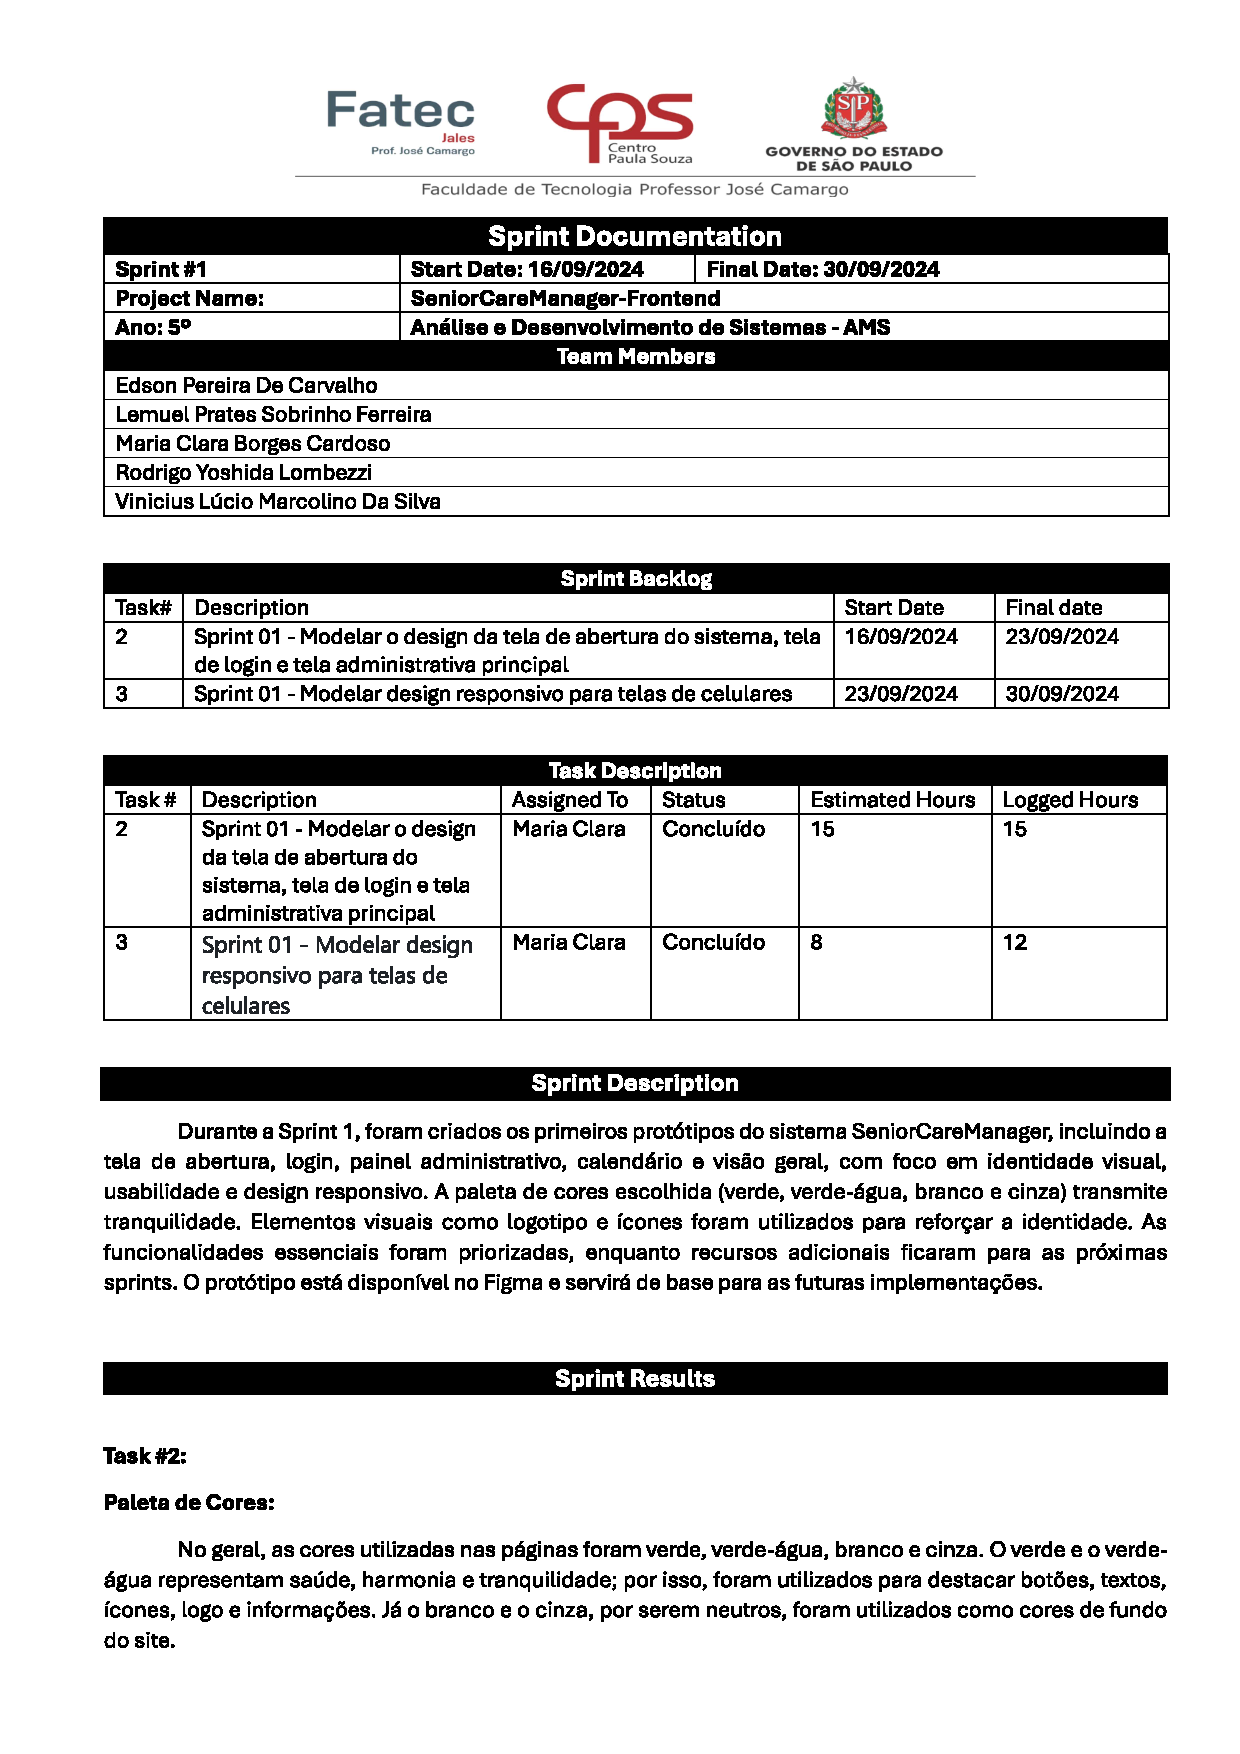
\includepdf[
	scale=0.8,
	pages=1,
	pagecommand={\subsection{Sprint 01 - Task 02 e 03}}
	]{sprints/Sprint01_SeniorCareManager-Frontend_assinado.pdf}
	\includepdf[
	scale=0.8,
	pages=2-14,
	pagecommand={}
	]{sprints/Sprint01_SeniorCareManager-Frontend_assinado.pdf}
	
	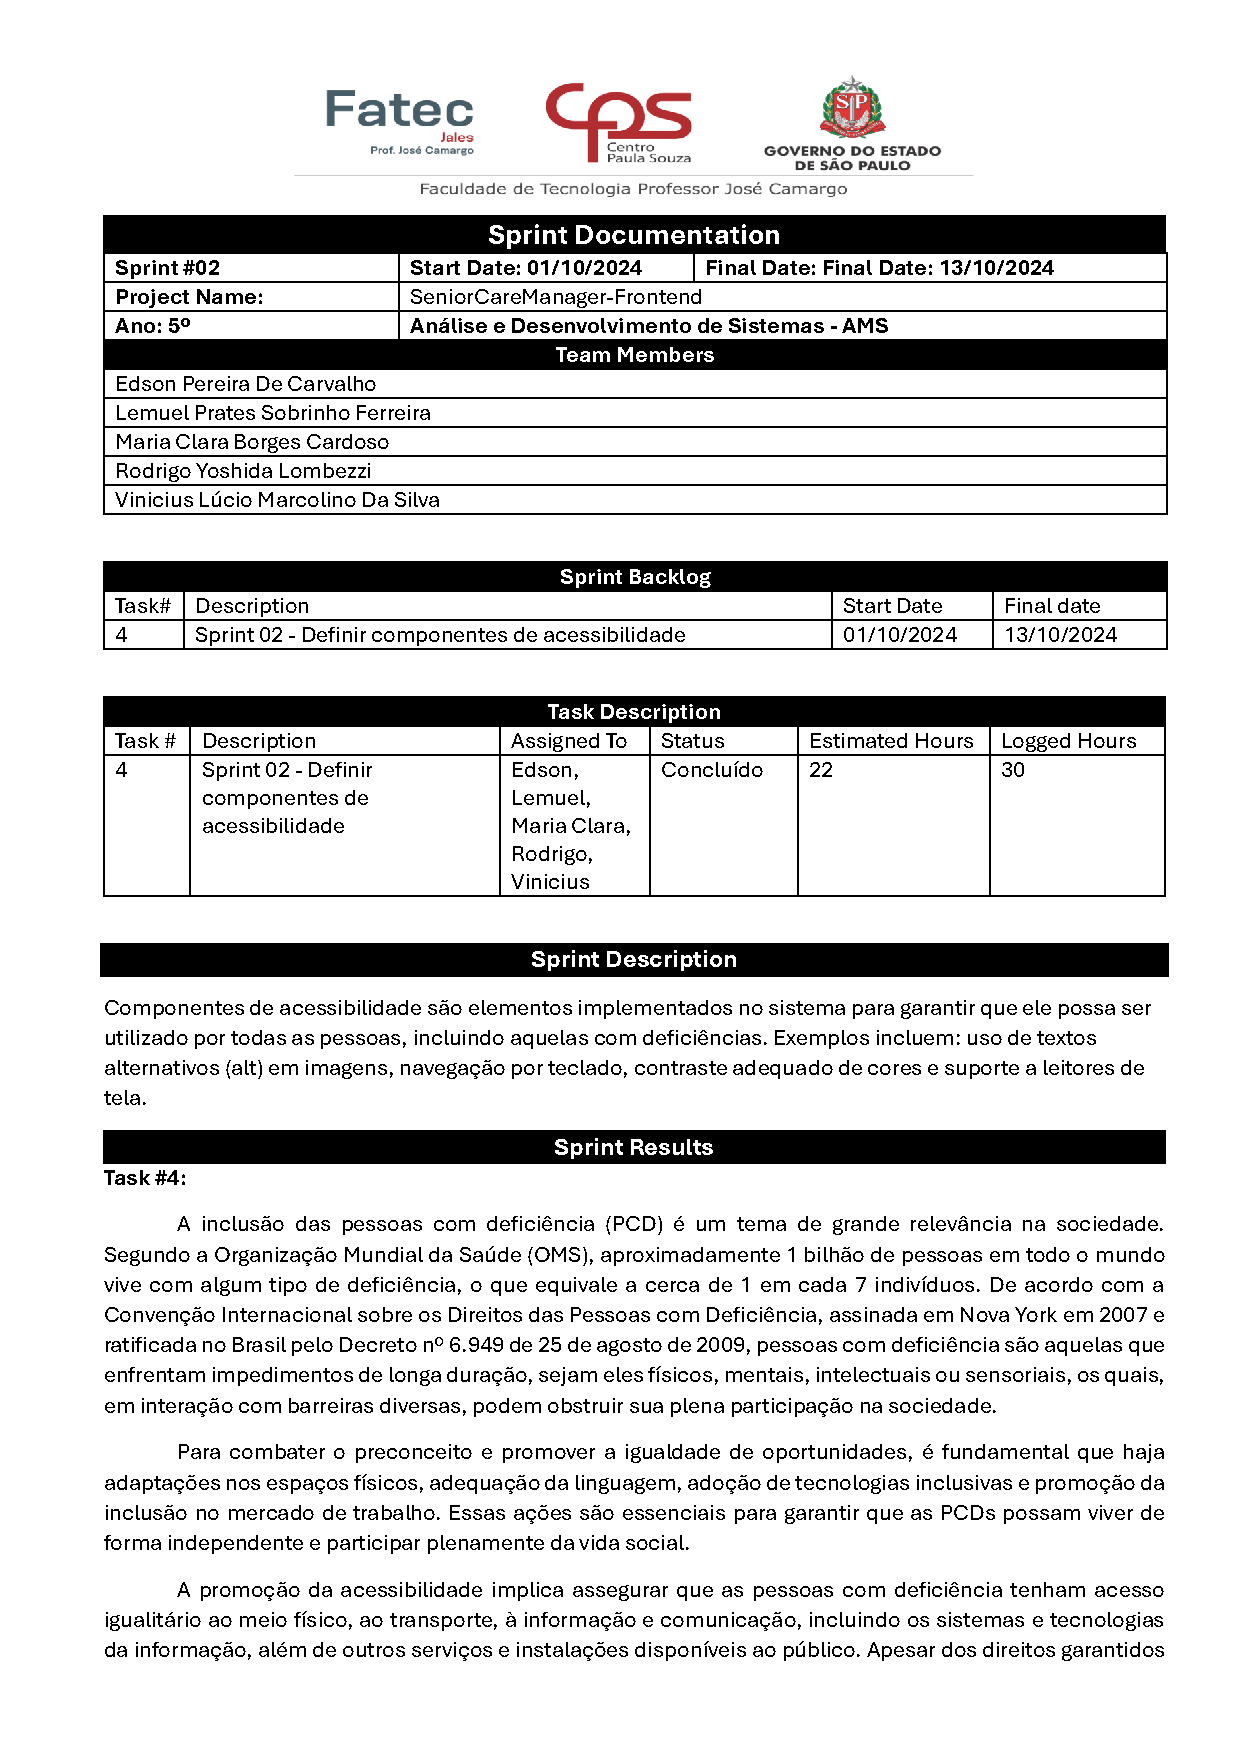
\includepdf[
	scale=0.8,
	pages=1,
	pagecommand={\subsection{Sprint 02 - Task 04}}
	]{sprints/Sprint02_SeniorCareManager-Frontend.pdf}
	\includepdf[
	scale=0.8,
	pages=2-18,
	pagecommand={}
	]{sprints/Sprint02_SeniorCareManager-Frontend.pdf}
	
	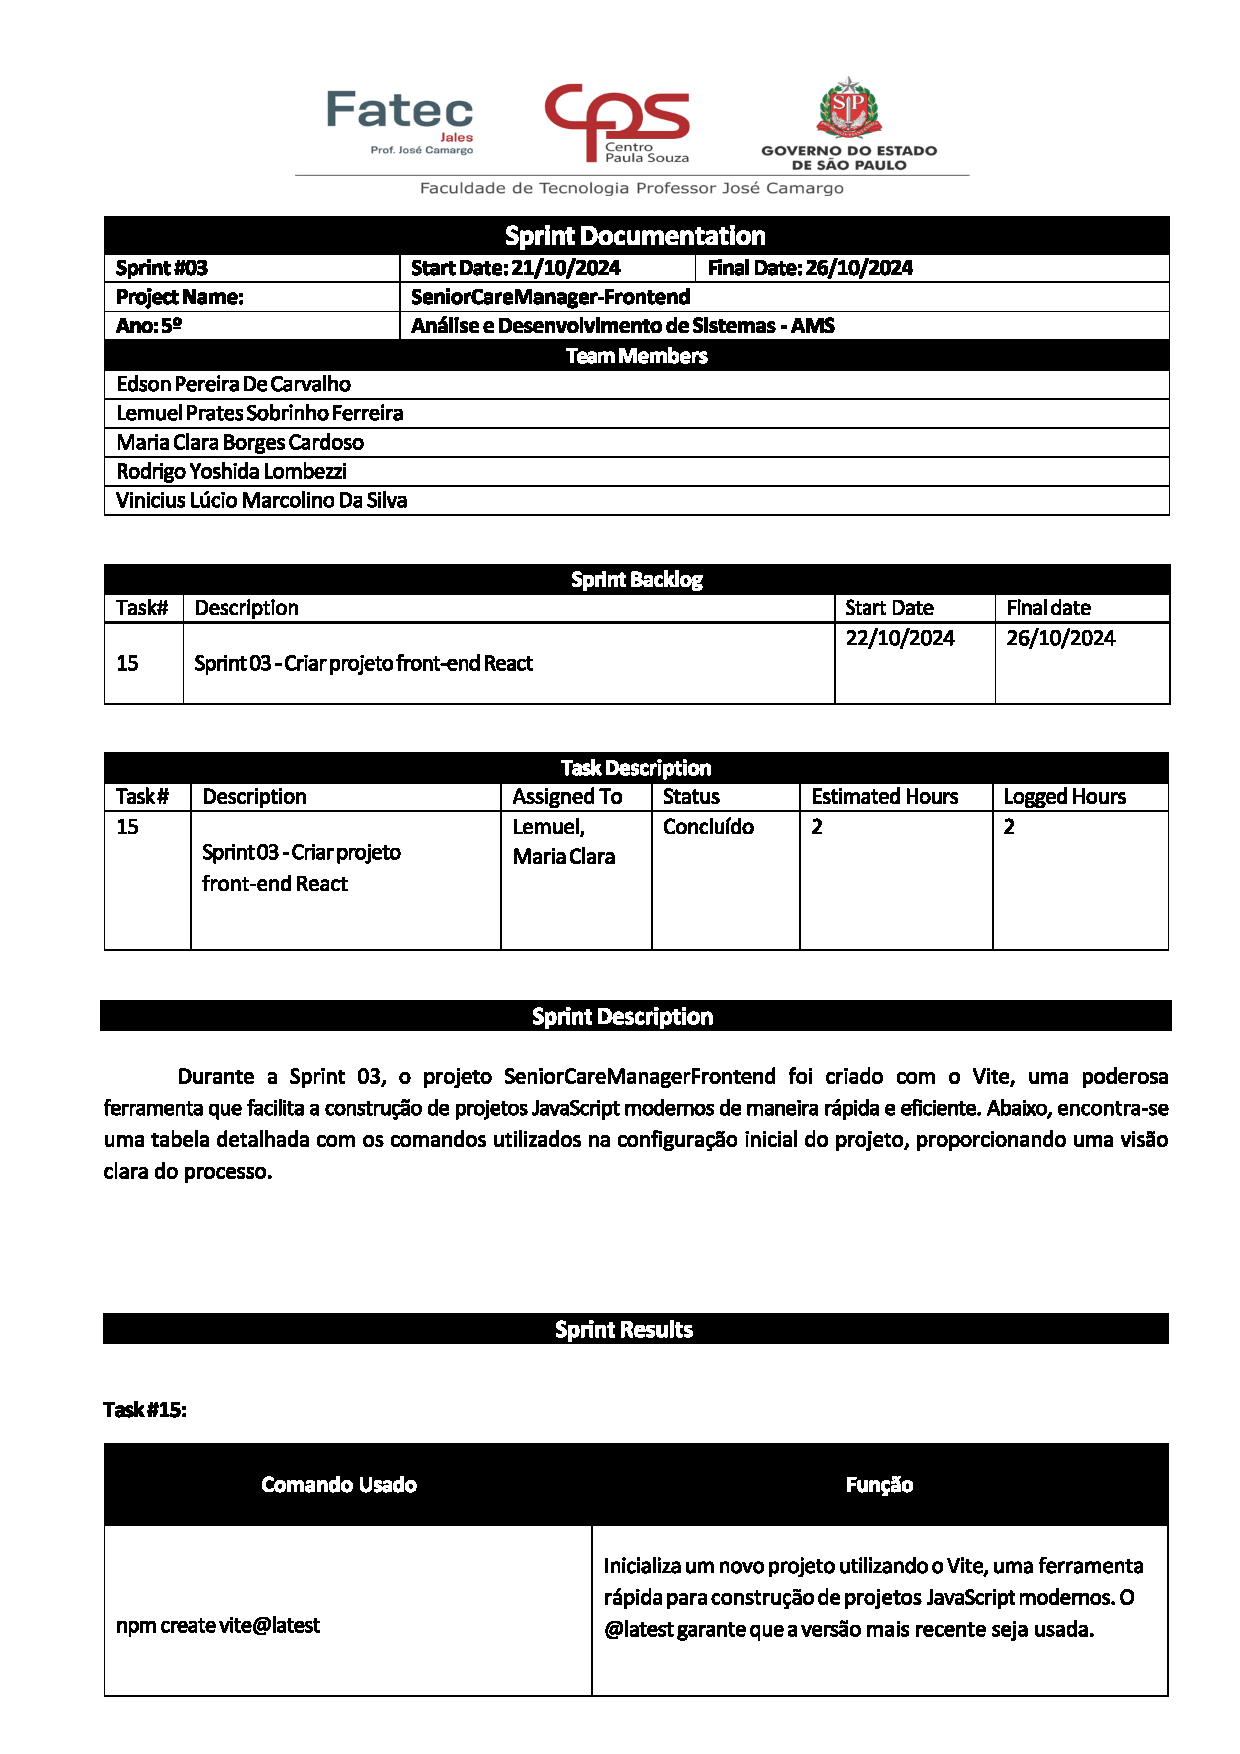
\includepdf[
	scale=0.8,
	pages=1,
	pagecommand={\subsection{Sprint 03 - Task 15}}
	]{sprints/Sprint03_SeniorCareManager-Frontend.pdf}
	\includepdf[
	scale=0.8,
	pages=2,
	pagecommand={}
	]{sprints/Sprint03_SeniorCareManager-Frontend.pdf}
	
	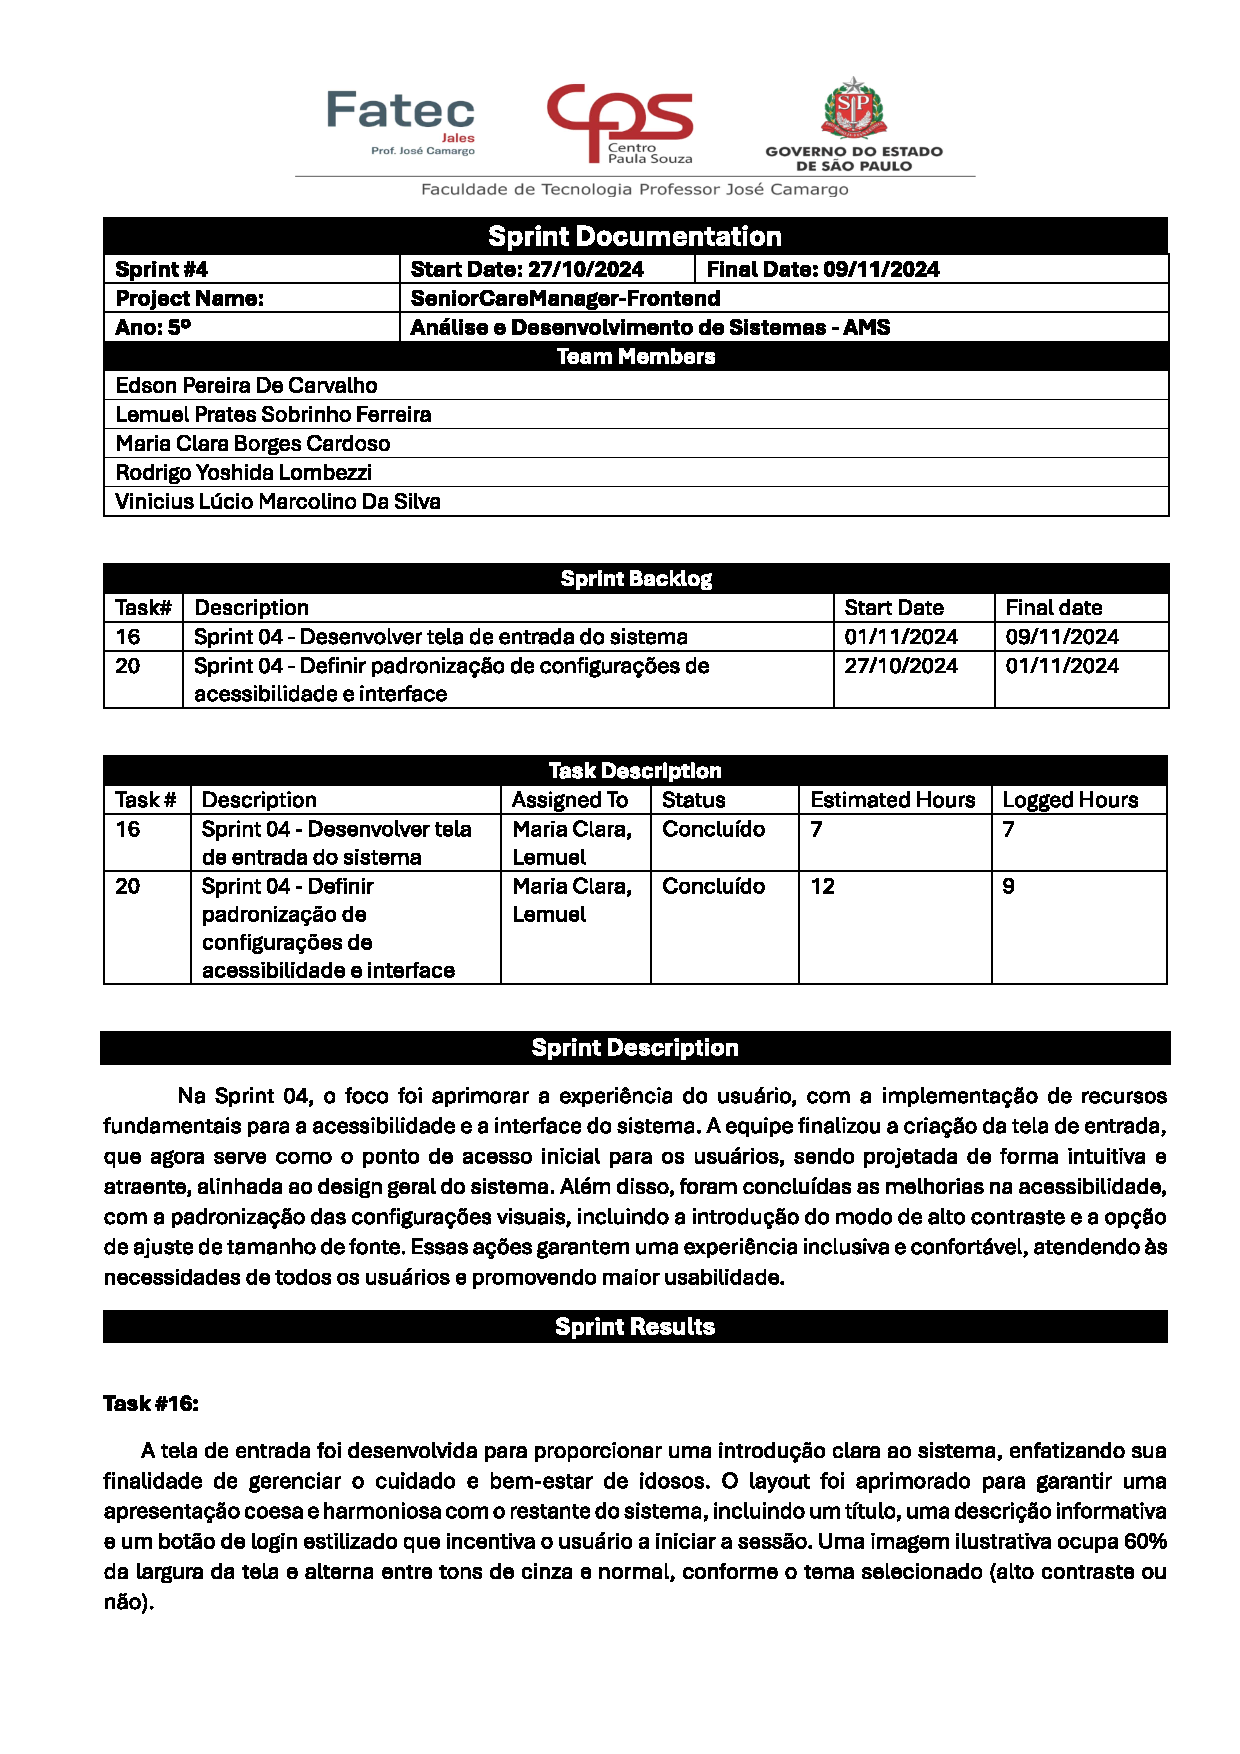
\includepdf[
	scale=0.8,
	pages=1,
	pagecommand={\subsection{Sprint 04 - Task 16 e 20}}
	]{sprints/Sprint04_SeniorCareManager-Frontend.pdf}
	\includepdf[
	scale=0.8,
	pages=2-9,
	pagecommand={}
	]{sprints/Sprint04_SeniorCareManager-Frontend.pdf}
	
	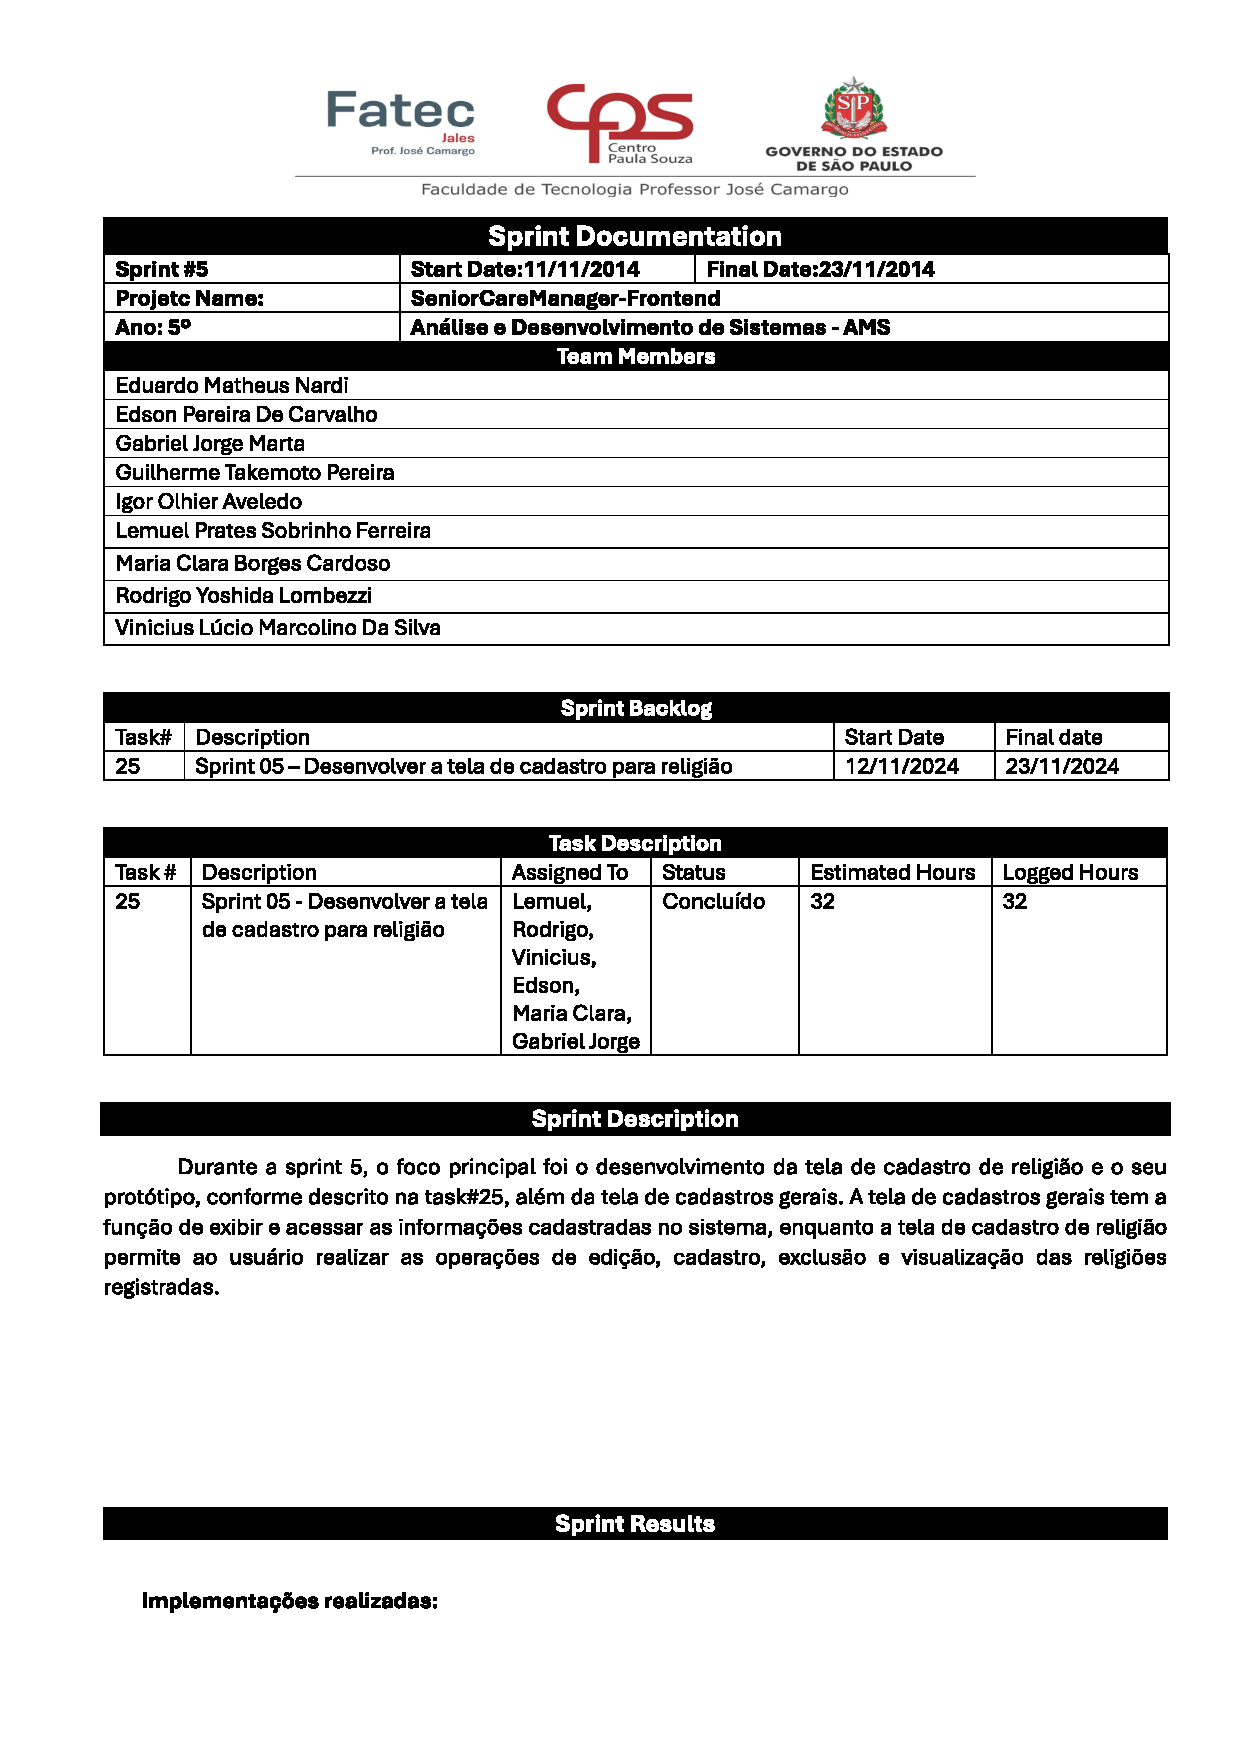
\includepdf[
	scale=0.8,
	pages=1,
	pagecommand={\subsection{Sprint 05 - Task 25}}
	]{sprints/Sprint05_SeniorCareManager-Frontend.pdf}
	\includepdf[
	scale=0.8,
	pages=2-9,
	pagecommand={}
	]{sprints/Sprint05_SeniorCareManager-Frontend.pdf}



% PARTE - Define a divisão do documento em partes (Não é obrigatório)
%\part{Preparação da pesquisa}
%\include{capitulos/referencias}
%\include{capitulos/estadodaarte}
%\include{capitulos/ferramentas}

% PARTE
%\part{Proposta}
%\include{capitulos/proposta}

% PARTE
%\part{Parte Final}
%\include{capitulos/resultados}
\chapter{Conclusão}

O desenvolvimento do sistema \textit{SeniorCareManager} demonstrou a relevância da tecnologia como ferramenta de fortalecimento institucional em organizações sociais. A partir da identificação das fragilidades operacionais do Lar dos Velhinhos São Vicente de Paulo e da APAE de Jales, evidenciou-se a necessidade de uma solução que integrasse informações assistenciais, administrativas e logísticas de forma segura e rastreável. O projeto resultou em uma plataforma robusta, composta por módulos independentes e intercomunicáveis, capazes de automatizar processos essenciais, como prontuário eletrônico, controle de estoque, compras, doações e gestão de vacinas.

A utilização de práticas consolidadas de engenharia de software, aliada à modelagem UML, possibilitou a definição clara de requisitos, fluxos e entidades, garantindo coerência estrutural e aderência às necessidades institucionais. Aspectos como acessibilidade, segurança da informação e conformidade com a LGPD reforçaram o compromisso do projeto com a proteção de dados e a inclusão tecnológica.

Assim, o \textit{SeniorCareManager} representa um avanço significativo na modernização das rotinas internas das instituições atendidas, contribuindo para maior eficiência operacional, qualidade assistencial e otimização de recursos. O projeto reafirma o potencial transformador da extensão acadêmica, ao integrar conhecimento técnico e impacto social.


% ----------------------------------------------------------
% ELEMENTOS PÓS-TEXTUAIS (Referências, Glossário, Apêndices)
% ----------------------------------------------------------
\postextual

% Referências bibliográficas
%\bibliographystyle{abntex2-alf.bst}
%\bibliography{bibliografia}
\printbibliography[heading=bibintoc,title={Referências}]


% Glossário (Consulte o manual)
% \glossary

% Apêndices
% \include{postextual/apendices}

% Anexos
%\include{postextual/apendice}

% Índice remissivo (Consultar manual)
% \phantompart
% \printindex

\end{document}
